
\lhead{\emph{Quantification of AMC Prototype}}


\chapter{Quantification of Active Magnetic Compensation Prototype}\label{ch:quantification}


In Chapter~\ref{ch:operation}, the magnetic control process and the
simulation methods to understand the process have been described. The
quantitative measures of the magnetic field compensation performance
suggested by the Refs.\cite{bea,lins,rawlik} are also discussed
there. While implementing the magnetic control process discussed in
Chapter~\ref{ch:operation}, we have faced problems in terms of long
drift in the coil currents and also slower response of the prototype
system. We have been able to make the system faster by introducing
filter which enables us to change the sample frequency without adding
noise and will be discussed in Section~\ref{sec:freq}. In
Section~\ref{sec:pi_behave}, we have discussed the studies to
understand P and I term of PI control algorithm. But the coil current
drifting problem is still there. We have then changed the fluxgate
positions randomly to try to make condition number smaller and we have
also removed the outermost passive shielding layer to see if there is
any effect. For confirming the experimental coil current pattern, we
have also made a simulation of the prototype. All the discussions
about the different position of fluxgates and shield removal are in
Section~\ref{sec:flux_place}. We have also implemented the new control
algorithm suggested by Ref.~\cite{rawlik} and compared with our
existing one suggested by Ref.~\cite{bea}. While comparing those we
came up with an interesting similarity in the control algorithms which
is discussed in Section~\ref{sec:style_pi}. But the new algorithm sill
had no answers for the current drifting problems which encouraged us
to study the regularization parameter in different way that is
discussed in Section~\ref{sec:new_study_r}. The current drifting
problem can be solved but that introduced additional noise. We have
then realized that coil configuration has a great impact on the
current modes which we have discussed in
Section~\ref{sec:coil_config}. Finally, the results of the metrics
that has been discussed in Section~\ref{sec:metrics} are presented in
Section~\ref{sec:metrics_res}. There are some unique points discussed
here which are not explicitly present on previous studies on active
compensation. These represent the principal improvements and
innovations made in this thesis work.  They are: {\color{red}These
should be made to sound impressive and potentially gathered together
to make a smaller list.}
\begin{itemize}
    \item a new $\mathbf{4^{th}}$ order low pass Butterworth filter
    \item PI tuning general behaviour on active compensation system 
    \item $r$ behaviour on PI tuning.
    \item Effect of $r$ on coil current response
    \item Impact of shield on active compensation
    \item Fluxgate placement suggestions.
    \item Relation of $r$ with matrix condition number
    \item Prototype PI control simulation
    \item Relation of different PI control algorithm
    \item Coil current modes based on coil configuration
\end{itemize}
New directions for future studies are presented in
Chapter~\ref{ch:conclusion}.

% we have the varied some parameters to quantify the prototype system. They are 
% \begin{itemize}
%     \item Sampling frequency
%     \item $r$, P and I term
%     \item 
% \end{itemize}

% There are vast number of parameters that can be varied and studied for active compensation. For quantifying the the prototype, five among them are chosen based on importance, time limitation, resources available etc. and studied via both experiment and simulation. Those will create a huge impact for the future studies on active compensation. Some unique points have been discussed which aren't explicitly present on previous studies on active compensation. Their successfulness have been discussed using some metrics (see Section~\ref{sec:metrics}). In this chapter, studies on the parameter as well as the metrics to justify them will be discussed in terms of results.

\section{Sampling Frequency and Filtering}\label{sec:freq}

%\begin{itemize}
%\item We built some analog filters which were discussed in Chapter 3
%\item Goal of the filter was to remove high-frequency noise (low-pass Butterworth with 10~Hz corner frequency)
%\item This would allow the ADC to operate with less averaging, reducing its effective sampling time (denoted by the ``resolution index'')  (refer to Ch. 3)
%\item We show the effectiveness in this section.
%\end{itemize}

In Chapter~\ref{ch:amcP}, I discussed new low-pass analog Butterworth
filters which I built and implemented into the system.  The filters
were designed with 10~Hz corner frequency with the goal to remove
high-frequency noise.  This would allow the ADC to operate with less
averaging, increasing its effective sampling frequency (denoted by the
``resolution index'' in Table~\ref{table:t7freq}).  The filter gives
us more freedom in terms of
\begin{itemize}
    \item using different sampling frequencies of the ADC,
    \item reducing magnetic field compensation response time,
    \item reducing coil current response time, and most importantly
    \item maintaining our design sample rate with better reduction of noise.
\end{itemize}
My studies of the effectiveness of the filters in achieving these
points are described in this section.



% \subsubsection{Filtering effect to use the fastest sampling frequency}

%\begin{itemize}
%\item Fix Fig. 5.1 (horizontal scale)
%\item Without filter noise is dominated by 60 Hz and higher.
%\item Compensation is off
%\item Also compared with SCU... it agreed well.  Our filters gave slightly better performance (lower noise) likely due to slight difference in design.
%\item Loop frequency is 100~Hz.  This is larger than 25~kHz$/14\approx 2$~kHz reported in Chapter 3 (ref) because of polling time.  Typ.~1~ms/channel read.  When read in this way, can increase resolution index to 7 (and averaging time) before significant delays are noted.  (when ADC effective sample time approaches 1~ms)
%\item At times we did this alternate way:  increase resolution index.
%\item Another problem:  current drifting during compensation although field would not change.  This is discussed further in Sections~\ref{drifting1} and \ref{drifting2}.
%\item We thought maybe this was due to sequential reads (higher resol index $\sim$ 7) so in general we aimed for resol index 1 which makes the reads distributed in time.  (Explain better... it is leading up to Fig. 5.2 and 5.3.)  In such cases when using lower resol index (1) we did software averaging until the design loop rate was met.  This will be discussed further in the next sections.
%\item Another point:  in Fig. 5.1 is that there is a time lag (slewing?) for the filter... consistent with expectation.
%\item Conclusion:  the filter works and allows us to go to higher effective sample rate.
%\item We would be stuck at resolution index 11 or 12 otherwise.  12 has 6 Hz effective sample rate $\approx$ 10 PLC averaging.  If doing this for 12 channels it it means $<0.5$~Hz.  Impossible to do compensation at 6~Hz this way (fails to meet design goal).
%\end{itemize}

Without the filters, the noise on the fluxgate signals are dominated
by 60~Hz and higher frequency noise.  As a consequence, resolution
index 11 or 12 was always used in order to remove this noise.
Resolution index 12 would correspond to averaging over roughly 10
power line cycles (PLC), as indicated in Table~\ref{table:t7freq2},
and would therefore significantly reduce the noise.  The problem with
this solution is that the feedback and control loop cycle time for all
14 ADC channels would be limited to $\sim 0.5$~Hz, which does not meet
the design goal of $\gtrsim 6$~Hz.

\fig{Images/filtering2}{width=\textwidth}{Filtering effect on the magnetic field signal measured at the 1x position.  For this measurement, the PI control system was switched off so that it would not affect the noise.  Vertical axis represent $\Delta B$ (see Eq.~(\ref{eq:del_B})) found from the measurement of sensor (a) without filter, (b) with Bartington's SCU1 (Signal Conditioning Unit) and (c) with our filter. Vertical dashed lines indicate the time of the perturbation coil being turned on and off.  The current supplied on perturbation coil was 100~mA and resolution index 1 was used for the ADC. The loop sampling frequency for (a), (b) and (c) are shown in Hz and is limited by the polling time for the 14 sensors.\label{fig:filtering}}{Filtering effect on the magnetic field signals.}

Fig.~\ref{fig:filtering} shows an example of the importance of using
the filter, comparing an unfiltered signal to one filtered by
Bartington's SCU1 10 Hz low pass filter, and comparing with our
filter.  For this study the fastest effective sampling rate
(resolution index 1) has been used.  The loop sampling frequency is
found to be $\sim 220$~Hz limited by the polling time for all 14
channels and additional delays arising from LabJack communications.

It is seen that the signal is very noisy without any filter. The noise
is reduced by a factor of ten using Bartington's SCU1 10 Hz low pass
filter.  Our filters gave slightly better performance (lower noise)
than the Bartington SCU1 module, likely due to slight differences in
components and design.  It is also seen that the outputs are limited
in their time response by the filters, as expected.

% When read in this way, the resolution index can be increased to 7 before significant delays are noted which is the same time when ADC loop sample time approaches 1~ms. We thought maybe this was due to sequential reads (higher resol index $\sim$ 7) so in general we aimed for resol index 1 which makes the reads distributed in time.  (Explain better... it is leading up to Fig. 5.2 and 5.3.)  In such cases when using lower resol index (1) we did software averaging until the design loop rate was met.  This will be discussed further in the next sections.

% In the early days of the prototype experiment, we have used the slowest sampling frequency which is corresponding to resolution index 12 in Table~\ref{table:t7freq} to get rid of high frequency noise e.g. 60 Hz and higher.
% While converting anlog dc fluxgate signal When determining the value of a dc signal, there oftentimes exists some power line-induced ac noise. Integrating the dc signal over one or more power line cycles helps to reject this noise. If the noise is at the line frequency (60Hz in the U.S., 50Hz in most other countries), it can be removed over one cycle. Sometimes however, the noise is not uniform, and the signal should be integrated over multiple cycles. The greater the number of power line cycles, the more accurate the signal value will be, i.e. greater noise rejection and better resolution. If your application simply calls for a true/false or high/low voltage reading, minor noise will not be a major factor in achieving the desired value, and you can use a very small NPLC to maximize throughput.






% Sampling frequency is the number of samples per second in a signal. For the prototype, by sampling frequency we meant that the number of signals of the fluxgate sensors that are going to the feedback algorithm via analog to digital converter (ADC) per second per measurement. But we are recording the time for a complete iteration which we call it as loop sampling frequency which includes the ADC sampling frequency plus rest of the loop frequency.   The problem with that was the response time for the current was very slow and so does the compensation of the magnetic field. Then we have decided to use the fastest sampling frequency that the ADC can offer which is corresponding to resolution index 1 in Table~\ref{table:t7freq}. But new problem has arisen in terms of noise especially the 60 Hz electrical noise from the power source which has motivated us to build the 4\textsuperscript{th} order low pass Butterworth filter (see Section~\ref{sec:filter}) to get rid of unwanted high frequency noise. This Section talks about the results that we got to solve those problems by increasing the sampling frequency.



% As we have decided to use the fastest sampling frequency that our ADC
% can offer as discussed above , we have faced problems in terms of
% noise there. So, we have build a 4\textsuperscript{th} order low pass
% Butterworth filter (see Section~\ref{sec:filter}) to get rid of
% unwanted high frequency noise.



%
% The Fig.~\ref{fig:filtering} shows the importance of using the filter discussed above. The data was taken by measuring the drift in the signal $\Delta B$ (see Eq.~(\ref{eq:del_B})) by '1x' sensor position two times where one with filter and another one without filter. On the part of data measurement, current has been applied in the perturbation coil at $\sim$ 0.32 s which is indicated by the vertical red dashed line and is termed as ON. At $\sim$0.95 s current supply in the perturbation coil has cut off which is indicated by the green vertical dash line and termed as OFF. The total loop sampling frequency is found to be $\sim$220 Hz. It is seen that the signal is very less attenuated while using filter and very noisy without any filter.

The conclusion is that the filter is capable of reducing high
frequency noise and allows us to go to higher effective sample rate.
Given this additional freedom we can even do additional software
averaging within the feedback and control loop in order to further
reduce the noise.

%

% So, for faster sampling it needs to have filter to avoid high frequency noise. Next, after applying filter let's see how the sampling frequency has impact on response time of the magnetic field compensation.


% \subsubsection{Effect on Response Time of Magnetic Field Compensation}

%\begin{itemize}
%\item Fig. 5.2.  Left: with filter, resol index 1, 50 software averages per point, compensation ON, loop cycle rate (correction rate) 6.57 Hz indicated in the Fig.  Right:  no filter, resolution index 12, no other averaging (other than what the ADC oes), graph is on longer timescale because loop rate is slower (0.45~Hz).  Corrected/uncorrected (projected) values are shown.
%\item Main point:  loop cycle rate is good!  $\sim$ 15x faster.  Even plenty of time for additional averaging to reduce noise further.  Likely the same result if somewhat higher resolution index used, possibly even with reduced software averaging.
%\end{itemize}

\fig{Images/samp_freq_iteration}{width=\textwidth,height=8cm}{Magnetic field at sensor position 1y using resolution index 1 with 50 software averages per cycle (left) and resolution index 12 (right) when the active magnetic compensation system is switched on.  Blue curves:  measured field change $\Delta B$.  Red curves:  predicted uncompensated field change. Vertical dashed lines indicate the time of the perturbation coil being turned on and off. \label{fig:samp_freq_iteration}}{Active magnetic field compensation at sensor position 1y.}

Fig.~\ref{fig:samp_freq_iteration} shows an example of using the
filters with the active compensation system switched on (left).  Only
one of the 14 sensors being used in the system has been displayed.  In
this case, 50 software averages could also be conducted, achieving a
loop cycle rate of 6.57~Hz.  This can be compared with the right panel
of Fig.~\ref{fig:samp_freq_iteration}, where the analog filters were
not used, necessitating PLC averaging using the largest resolution
index of the ADC.  In this case a loop cycle rate of 0.45~Hz is
achieved.  Although both schemes achieve similar noise performance,
the analog filtering solution can increase the loop cycle rate by a
factor of $6.57/0.45\approx 15$.  The two panels of
Fig.~\ref{fig:samp_freq_iteration} appear on different time bases
because the number of feedback control loops has been equalized.

%\begin{itemize}
%\item Fig. 5.3.  Always filtered.  Different resolution indices indicated on the figure along with their loop cycle rates.  Always 50 software averages done.
%\item By resolution index 8 or 9, the loop cycle rate for the 50 software averages slows to 1.1 and 0.39 Hz respectively.  The results look similar to resolution index 12 (without filter) but much less noisy, smoother.
%\item Another option is to run with fewer averages than 50 and at higher resolution index, while still achieving the 6 Hz loop rate design goal.  This would likely also work just fine although we didn't try it.  The advantage of resolution index 1 with averaging is that the channels are all sampled at closer to the same time, which we suspected was a problem, as discussed earlier.
%\end{itemize}


Another significant problem that I faced in this experiment was that
the current would drift during compensation although field would not
change significantly.  This is discussed further in Sections~\ref{sec:pi_behave}, \ref{sec:flux_place}, and \ref{sec:pSim}.  For this reason, I was
often concerned with any sources of slow current response.  The main
point of the remainder of this section is to study the trade-offs
involved in the resolution index, the loop cycle rate, and the number
of software averages, and their effect on changes in the coil currents
driven by the compensation system.

\fig{Images/samp_freq_time}{width=\textwidth,height=8cm}{The $C_x^-$ coil current (left) and magnetic field $\Delta B$ (right) for sensor 8x for various resolution indices.  The resolution indices are represented by 1, 6, 7, 8 and 9 with the corresponding loop sampling frequencies indicated.  In each case, 50 software averages were done in the loop as well.  Vertical dashed lines indicate the perturbation coil state. \label{fig:samp_freq_example_time}}{Compensation behaviour for various resolution indices.}

Fig.~\ref{fig:samp_freq_example_time} shows an active compensation
result displaying the current in one of the 6 coils and the field in
one of the 14 fluxgate axes, when the resolution index is changed.
For each case, 50 software averages have always been done in the
feedback loop, further reducing the loop cycle rate.  Increasing the
resolution index slows the response of the system, and most notably
the current response time increases.  For example, it takes $\sim 7$~s
for the $C_x^-$ coil current to settle after the perturbation coil is
switched on when the loop sampling frequency is 6.35 Hz. It is also
seen that the loop cycle rate slows to 1.1 Hz and 0.39 Hz by
resolution index 8 and 9 respectively.  The results look similar to
resolution index 12 (without filter) but are generally much less
noisy, and smoother over longer periods of time as well.


\fig{Images/samp_freq_same}{width = \textwidth,height=8 cm}{Active magnetic field compensation for resolution indices 1, 3, 5 and 7 and for 50, 45, 29 and 13 software averages respectively.  These settings achieve nearly the same loop cycle rates ($\sim 6$~Hz, indicated in parentheses).  Only the $C_x^-$ coil current (left) and $\Delta B$ for fluxgate 8x (right) are shown.  Vertical dashed lines indicate the time of the perturbation coil being turned on and off. \label{fig:samp_freq_same}}{Compensation behaviour for various resolution indices with different software averages.}

Another option is to run with fewer averages than 50 and at higher
resolution index, while still achieving the 6 Hz loop rate design
goal.  Fig.~\ref{fig:samp_freq_same} shows a study where, as the
resolution index is increased, the number of software averages is
decreased, so as to maintain nearly the same $\sim 6$~Hz loop cycle
rate.  As expected, they all have a similar effect on the magnetic
compensation result.  But the coil current and magnetic field for
resolution index 7 is noisier compared to others. 

We expect that the advantage of resolution index 1 with larger
software averaging is due to the fact that the 12 channels are sampled
more continuously over the entire course of one loop cycle.  This
potentially gives a more accurate measurement of the true magnetic
field, averaged over that cycle.


% 
% In the upcoming Section PI, regularization parameter and condition number will be revisited with results.

\section{PI Tuning General Behavior}\label{sec:pi_behave}
%Main points:
%\begin{itemize}
%\item Lead into discussion of the current-drifting problem and that since the simulation and data agree, and we checked the hardware, that it is not a hardware problem.
%\end{itemize}

The tuning method of proportional gain $k_c^p$ (P) and integral reset
$k_c^i$ (I) have been discussed in Section~\ref{sec:tune}, for example
in Eq.~(\ref{eq:I}).  This Section describes the effect of changing P
and I term individually and together on feedback system performance.

A problem that became more apparent in the course of these studies was
long-term drifting of the applied currents in the feedback system.  A
major conclusion of this section is that adjustments of the PI
parameters could not fix this problem, which is discussed further in
later sections.


\subsection{Effect of changing P term}

For these studies, the proportional gain $k_c^p$ was varied while the
integral reset $k_c^i$ was set to zero.  We expected that this would
result in a form of multidimensional proportional droop.  Proportional
droop occurs because the proportional term contains only the
instantaneous error function.  A controller using only P-control
therefore requires a non-zero error in order to function.  This
results in the error never being fully corrected and hence ``droop''.
Raising $k_c^p$ can decrease the droop but will eventually result in
system oscillation.

\fig{Images/p25p125}{width=\textwidth,height=12cm}{Currents (left) in all six coils ($C_x^\pm$, $C_y^\pm$ and $C_z^\pm$) and field change $\Delta B$ (right) for 12 fluxgate axes with fluxgate positions 1, 3, 6 and 8.  (a) $k_c^p=0.25$, (b) $k_c^p=1.25$.  In both cases $k_c^i=0$.  Grey curves denote the uncompensated $\Delta B$ whereas colors indicate the compensated values with one color denoting each axis.  Vertical dashed lines indicate the perturbation coil being turned on and off.\label{fig:p_pi}}{Coil currents with field change $\Delta B$ for different values of $k_c^p$.}


The effect of changing $k_c^p$ is shown in Fig.~\ref{fig:p_pi}.  The
current supplied to the perturbation coil was 10~mA when on.
Resolution index 1 with 50 averages per feedback loop iteration were
used.  The resultant loop sampling frequency was found to be $\sim
6.5$~Hz.

Increasing $k_c^p$ from 0.25 to 1.25 gives larger correction currents
and better reduction of the changes induced by the perturbation coil.
However this comes at the expense of larger oscillations at higher
frequency in both the currents and the fields for the larger value of
$k_c^p$.  Both effects are as expected based on proportional droop.

\fig{Images/mont_p}{width = \textwidth}{The effect of $k_c^p$ on (a) current error and (b) remaining field fluctuations with the system operating on fluxgate positions 1, 2, and 7 (9 axes of control).  Here, 100~mA current has been supplied in the perturbation coil.\label{fig:mont_p}}{The effect of $k_c^p$ on fluctuations.}

The aggregate effect of $k_c^p$ on the current error and remaining
field fluctuations, in another similar test, is shown in
Fig.~\ref{fig:mont_p}.  Measurements were conducted using the system
for various $k_c^p$.  Beyond $k_c^p\approx 1.3$, the system would
start to oscillate.  This is reflected in the RMS current error taking
a value of 200~mA, which is approximately the dynamic range of the
current sinks used to power the coils.

The ``remaining fluctuations'' $F$ shown in the right panel of
Fig.~\ref{fig:mont_p} are based on the reduction of the measured field
compared to the predicted uncompensated field.  When the system is
oscillating, both the measured and uncompensated fields are seen to
oscillate, which is inaccurate (the uncompensated field obviously
should not oscillate).  As a consequence the system believes it is
reducing the field fluctations when in fact it is inducing
oscillation.  This is the reason the fluctuations apparently decrease
in the right panel.

%%% Figure showing a bunch of different r's and P's is commented out
%%% for now... more important to show in the later section.

%%%%\fig{Images/mont_pr}{width = \textwidth}{The effect of changing $k_c^p$ and changing $r$ on current fluctuations (a) and remaining field fluctuations (b) for fluxgate positions 1, 2, and 7. Here, 100 mA current has been supplied in the perturbation coil. For position of the fluxgates  and coil see Fig.~\ref{fig:coil}.\label{fig:mont_pr}}{Short}


I also studied the effect of varying the regularization parameter $r$.
As expected, when $r$ is increased, it decreases the amount of the
control.  The proportional gain would therefore have to be increased
in order to provide compensation.  Further studies of the adjustment
of $r$ are presented in Section~\ref{sec:new_study_r}.

% \doublefig{Images/p25}{width =\textwidth,height =8cm}{with passive shielding layers. \label{fig:shield_opera2}}{Images/p125}{width = \textwidth,height =8cm}{without outermost passive shielding layer.\label{fig:noShield_opera}}{{Currents (left vertical axis) in all six coil sides ($C_x^\pm$, $C_y^\pm$ and $C_z^\pm$) with drift $\Delta B$ (right vertical axis) at sensor position '1x' for different values of $k_c^p$ with $k_c^i$ in Eq.~(\ref{eq:I}) being zero. Blue color curve denotes the actual drift in signal at position '1x' found by Eq.~(\ref{eq:del_B}) while the red curve denotes the drift that would have been without the compensation. Vertical dashed lines indicate the time of the perturbation coil being turned on and off. For position of coils and sensors see Fig.~\ref{fig:coil} \label{fig:p_pi}}}{Prototype setup in OPERA simulation software.}



% \begin{figure}[!htb]
%     \begin{subfigure}{.5\linewidth}
%         \centering
%         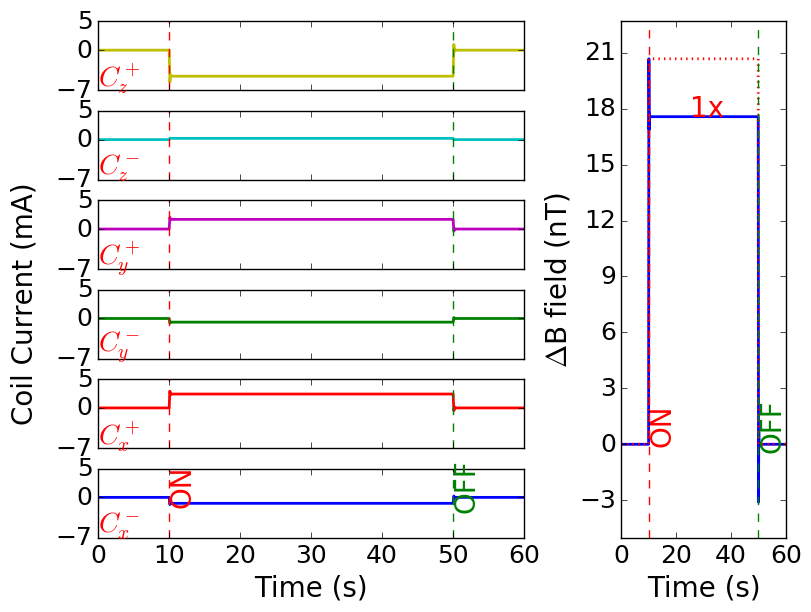
\includegraphics[width=\linewidth, height= 6.5 cm]{Images/p25_33}
%         \caption{at $k_c^p$=0.25}
%         \label{fig:p25}
%     \end{subfigure}%
%     \begin{subfigure}{.5\linewidth}
%         \centering
%         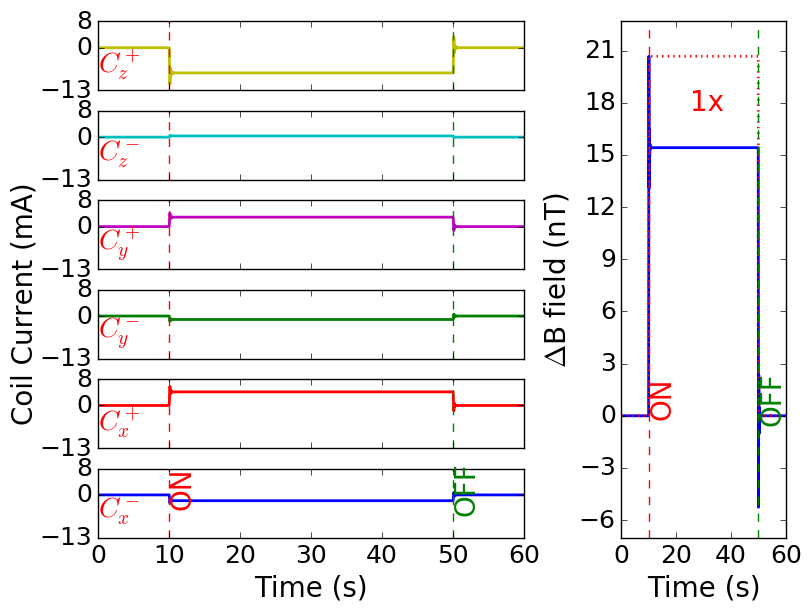
\includegraphics[width=\linewidth, height= 6.5 cm]{Images/p50_33}
%         \caption{at $k_c^p$=0.50}
%         \label{fig:p50}
%     \end{subfigure}\\[1ex]
%     \begin{subfigure}{.5\linewidth}
%         \centering
%         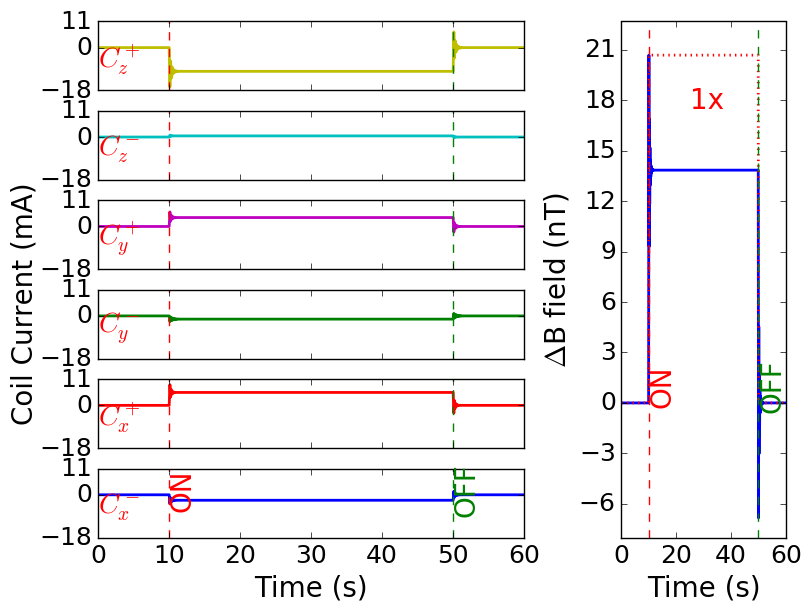
\includegraphics[width=\linewidth, height= 6.5 cm]{Images/p75_33}
%         \caption{at $k_c^p$=0.75}
%         \label{fig:p75}
%     \end{subfigure}%
%         \begin{subfigure}{.5\linewidth}
%         \centering
%         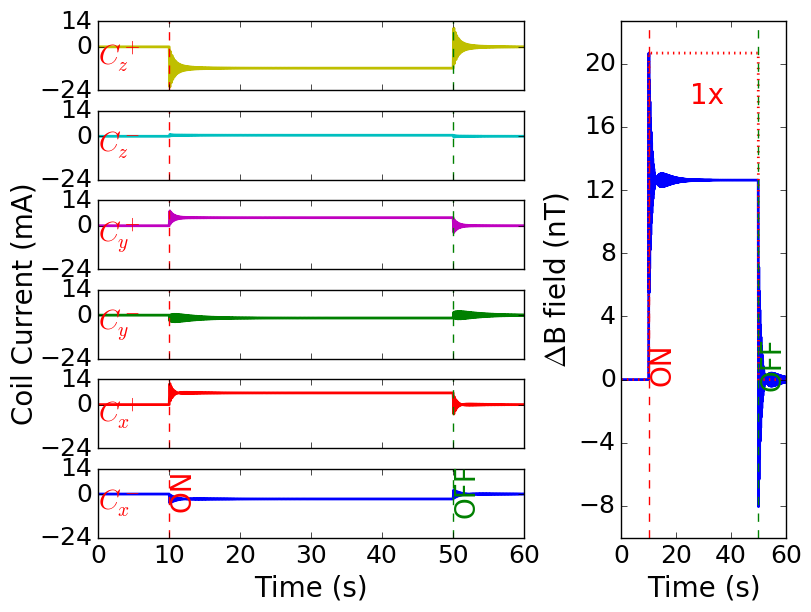
\includegraphics[width=\linewidth, height= 6.5 cm]{Images/p100_33}
%         \caption{at $k_c^p$=1.0}
%         \label{fig:p100}
%     \end{subfigure}

%     \caption[short]{Currents (left vertical axis) in all six coil sides ($C_x^\pm$, $C_y^\pm$ and $C_z^\pm$) with drift $\Delta B$ (right vertical axis) at sensor position '1x' for different values of $k_c^p$ with $k_c^i$ in Eq.~(\ref{eq:I}) being zero. Blue color curve denotes the actual drift in signal at position '1x' found by Eq.~(\ref{eq:del_B}) while the red curve denotes the drift that would have been without the compensation. Vertical dashed lines indicate the time of the perturbation coil being turned on and off. For position of coils and sensors see Fig.~\ref{fig:coil}. }
%     \label{fig:p_pi2}
% \end{figure}


% It is seen that $\Delta B$=17.5 nT, 15.5 nT and 13.5 nT for $k_c^p$ = 0.25, 0.5 and 0.75 respectively (see Fig.~\ref{fig:p_pi}\textcolor{blue}{(a)}, Fig.~\ref{fig:p_pi}\textcolor{blue}{(b)}, Fig.~\ref{fig:p_pi}\textcolor{blue}{(c)}). That is, with the increase of $k_c^p$, $\Delta B$ magnetic field decreases. But, it has a limit after which with the increase of $k_c^p$, the systems becomes unstable and starts oscillating which can be seen from Fig.~\ref{fig:p_pi}\textcolor{blue}{(d)}) where the currents (left) are oscillating and the drift itself also at $\Delta B$=12.5 nT (right). So, the error is reduced maximum by (20.5-12.5)/20.5 * 100$\%\approx$37$\%$ from the initial drift of $\Delta B$=20.5 nT denoted by the red curve at position '1x'. 

%
The above results confirm that increasing $k_c^p$ reduces difference
between the setpoint and the actual measurements of the magnetic
field, at least until the point when the system starts to oscillate.

\subsection{Effect of the I term}

In using integral reset, the error (the difference between setpoint
and actual measurement) is accumulated (integrated) over the series of
measurements.  The accumulated error keep tracks of the offsets
(proportional droop) that should have been corrected previously.  The
integral reset (I) term multiplies that accumulated error with a
constant gain $k_c^i$.

The value $k_c^i$ also determines how fast the feedback loop will
respond to changes in the error signal.  A large value of $k_c^i$ will
result in a faster response.  If $k_c^i$ is increased too much,
eventually it results in overshoot i.e. exceed the setpoint.

% As like the effect on P, the effect of changing I has been shown in Fig.~\ref{fig:i_pi} where the change in current in all six coil sides with  $\Delta B$ on a particular sensor position have been observed for $k_c^i$=0.25, 0.5, 0.75 and 1.0 . It is seen that with increase of I the level of compensation of the magnetic field is almost similar but the main difference occurs on how fast the system response in an expense of increasing current in all the coil sides (see Fig.~\ref{fig:i_pi}\textcolor{blue}{(a)}, Fig.~\ref{fig:i_pi}\textcolor{blue}{(b)}, Fig.~\ref{fig:i_pi}\textcolor{blue}{(c)} and Fig.~\ref{fig:i_pi}\textcolor{blue}{(d)}). The main problem with changing only I term is that it creates a very slow current response time. But, in terms of compensation only changing I gives very good result. The slow current response can be minimized by decreasing the value of optimized $r$ (see Section~\ref{sec:r_pi} and Section~\ref{sec:r_currentResponse} ).

\fig{Images/i125}{width=\textwidth,height =7cm}{Currents (left) in all six coils with field change $\Delta B$ (right) at 12 fluxgate sensors with fluxgate positions 1, 3, 6 and 8 for $k_c^i$=1.25 with $k_c^p=0$.  Grey curves denote the uncompensated field change while color curves denote the measured field change.  Vertical dashed lines indicate the perturbation coil being turned on and off.\label{fig:i_pi}}{Coil currents with field change $\Delta B$ for $k_c^i$.}

% \begin{figure}[!htb]
%     \begin{subfigure}{.5\linewidth}
%         \centering
%         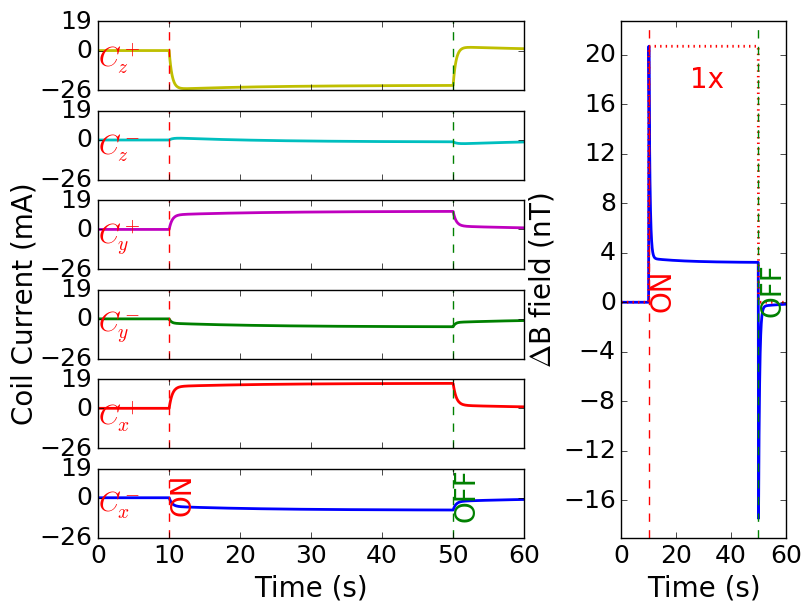
\includegraphics[width=\linewidth, height= 6.5 cm]{Images/i25_33}
%         \caption{at $k_c^i$=0.25}
%         \label{fig:i25}
%     \end{subfigure}%
%     \begin{subfigure}{.5\linewidth}
%         \centering
%         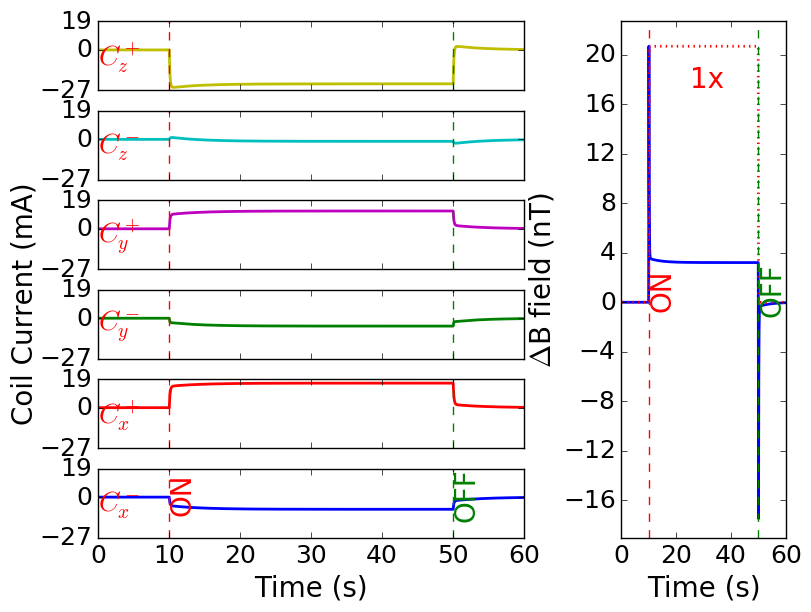
\includegraphics[width=\linewidth, height= 6.5 cm]{Images/i75_33}
%         \caption{at $k_c^i$=0.75}
%         \label{fig:i50}
%     \end{subfigure}\\[1ex]
%     \begin{subfigure}{.5\linewidth}
%         \centering
%         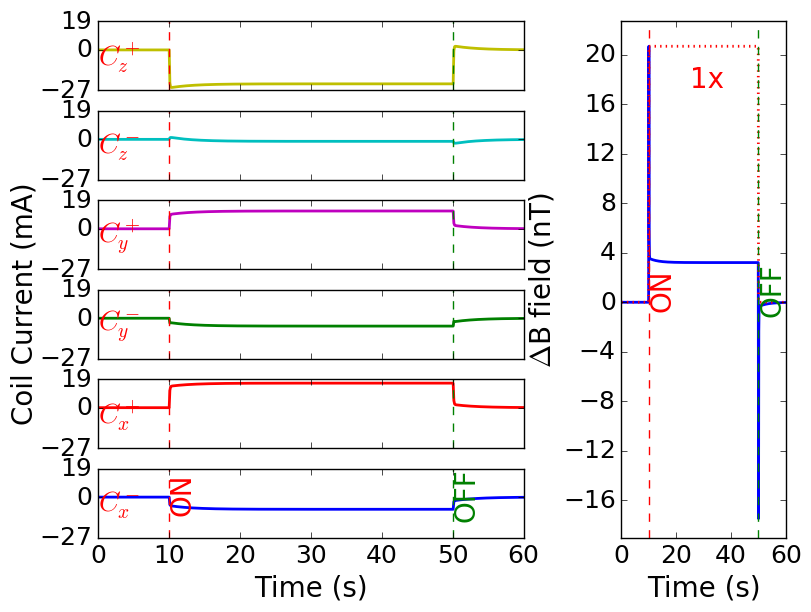
\includegraphics[width=\linewidth, height= 6.5 cm]{Images/i100_33}
%         \caption{at $k_c^i$=1.0}
%         \label{fig:i75}
%     \end{subfigure}%
%         \begin{subfigure}{.5\linewidth}
%         \centering
%         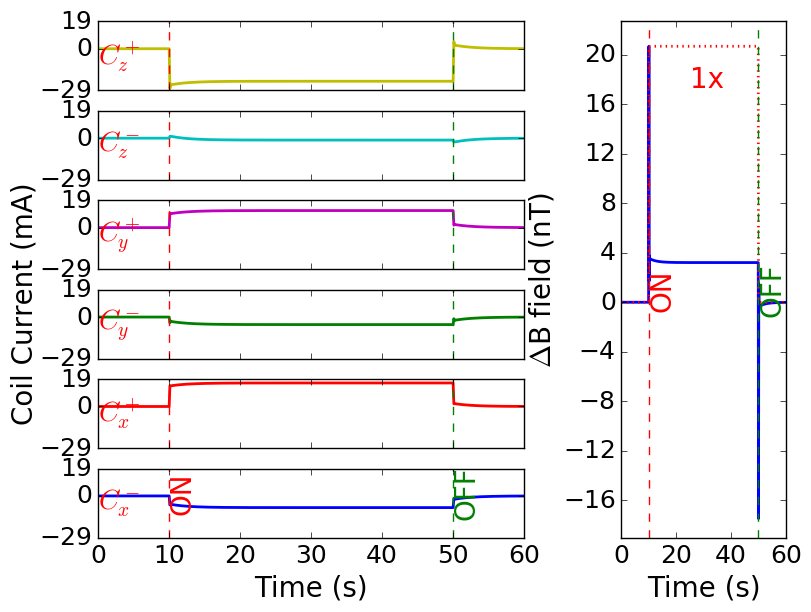
\includegraphics[width=\linewidth, height= 6.5 cm]{Images/i125_33}
%         \caption{at $k_c^i$=1.25}
%         \label{fig:i100}
%     \end{subfigure}

%     \caption[short]{Currents (left vertical axis) in all six coil sides ($C_x^\pm$, $C_y^\pm$ and $C_z^\pm$) with drift $\Delta B$ (right vertical axis) at sensor position '1x' for different values of $k_c^i$ with $k_c^p$ ( see Eq.~(\ref{eq:I}) ) being zero. Blue color curve denotes the actual drift in signal at position '1x' found by Eq.~(\ref{eq:del_B}) while the red curve denotes the drift that would have been without the compensation. Vertical dashed lines indicate the time of the perturbation coil being turned on and off. For position of coils and sensors see Fig.~\ref{fig:coil}.}
%     \label{fig:i_pi}
% \end{figure}

In this study I tried running the system with $k_c^p=0$ and then
adjusting $k_c^i$.  The results are shown in Fig.~\ref{fig:i_pi}.  As
for Fig.~\ref{fig:p_pi}, the current supplied to the perturbation coil
was 10~mA when it was switched on.  Resolution index 1 with 50
averages per feedback loop iteration were used.  The resultant loop
sampling frequency was found to be $\sim 6.5$~Hz.

A reasonably good value of $k_c^i=1.25$ was used for
Fig.~\ref{fig:i_pi}.

It is seen that coil currents range from 137 mA to 85 mA, which is a
large spread compared to Fig.~\ref{fig:p_pi}. It is also seen that the
range of $\Delta B$ is smaller indicating better compensation.  In
contrast to the right panel of Fig.~\ref{fig:p_pi}, the results in
Fig.~\ref{fig:i_pi} have reduced high-frequency noise.  So clearly
this is a system that is operating in a better state than
proportional-only control.

The other observation is that in the left panel of
Fig.~\ref{fig:i_pi}, the currents drift for very long periods of time.
This may be contrasted with the right panel of Fig.~\ref{fig:i_pi},
where it is clear that the fields do not drift with such long
timescales.  This can also be compared with Fig.~\ref{fig:p_pi} where
no such long-term drift of the currents can be seen either.

Eventually we figured out this problem was due to ill conditioning,
and it is discussed further in Section~\ref{sec:coil_config}.  But at the
stage we decided to characterize the problem further by adjusting the
PI parameters to see what effect that might have.

% \begin{itemize}
%     \item message from the Fig.~\ref{fig:i_pi} ?
% \end{itemize}

%

% \doublefig{Images/i100_33_zoom}{width =\textwidth,height =8cm}{at $k_c^i$=1.0 \label{fig:shield_opera2}}{Images/i125_33_zoom}{width = \textwidth,height =8cm}{at $k_c^i$=1.25 \label{fig:noShield_opera}}{{Simulated zoomed version of the drift $\Delta B$ for fluxgate position 1x for different values of $k_c^i$ with $k_c^p$ ( see Eq.~(\ref{eq:I}) ) being zero. For position of coils and sensors see Fig.~\ref{fig:coil}. For description about simulation see Section~\ref{sec:pSim}. The red vertical dashed line indicates the time of the perturbation coil being turned 'ON'. A time delay of 0.145 s was used to match the experimental loop sampling frequency of $\sim$6.5 Hz. \label{fig:i_pi_zoom}}}{Simulated zoomed version of the drift $\Delta B$.}

% For understating the system response time and the overshoot effect, two PI simulation as explained in Section~\ref{sec:pSim} with only $k_c^i$=1.0 and $k_c^i$=1.25 have been made and  each case $\Delta B$ graphs have been generated and zoomed as shown in Fig.~\ref{fig:i_pi_zoom}. It is seen that the $\Delta B$ is $\sim$3.23 nT  at 25-10=15 s (the perturbation is turned 'ON' at 10 s) in Fig.~\ref{fig:i_pi_zoom}\textcolor{blue}{(a)} for $k_c^i$=1.0  compare to within 10.6-10.0=0.6 s in Fig.~\ref{fig:i_pi_zoom}\textcolor{blue}{(b)} for $k_c^i$=1.25. So, the magnetic field reduction response time increases hugely with increase value of $k_c^i$. It is also seen from the Fig.~\ref{fig:i_pi_zoom}\textcolor{blue}{(b)} that there is an overshoot in the error level before it settles in.
% \begin{itemize}
%     \item message from the Fig.~\ref{fig:i_pi_zoom} ?
% \end{itemize}

% It is seen that the error level (right) seems to be $\sim$3.5 nT in every case and the coil currents(left) settle  faster for increasing value of $k_c^i$. The figures are neither helpful to understand the system response time nor the overshoot effect in the $\Delta B$ graph (right). 
% for the same duration of perturbation (here 'ON' at 11s and 'OFF' at 51s and so total 40s)
% \begin{figure}[!htb]
%     \begin{subfigure}{.5\linewidth}
%         \centering
%         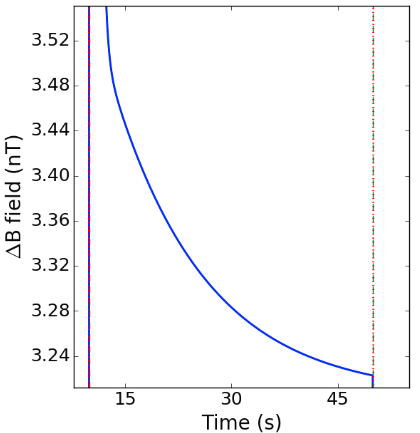
\includegraphics[width=\linewidth, height= 6.5 cm]{Images/i25_33_zoom.png}
%         \caption{at $k_c^i$=0.25}
%         \label{fig:i25zoom}
%     \end{subfigure}%
%     \begin{subfigure}{.5\linewidth}
%         \centering
%         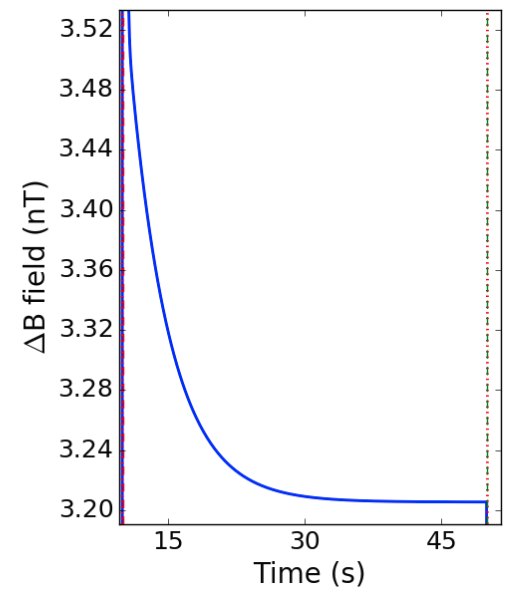
\includegraphics[width=\linewidth, height= 6.5 cm]{Images/i75_33_zoom.png}
%         \caption{at $k_c^i$=0.75}
%         \label{fig:i75zoom}
%     \end{subfigure}\\[1ex]
%     \begin{subfigure}{.5\linewidth}
%         \centering
%         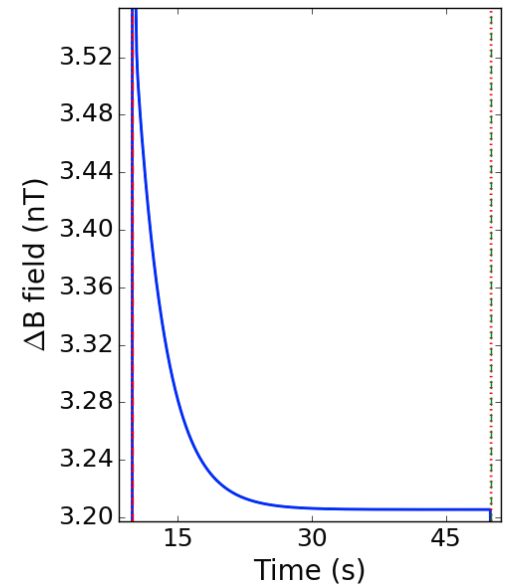
\includegraphics[width=\linewidth, height= 6.5 cm]{Images/i100_33_zoom.png}
%         \caption{at $k_c^i$=1.0}
%         \label{fig:i100zoom}
%     \end{subfigure}%
%         \begin{subfigure}{.5\linewidth}
%         \centering
%         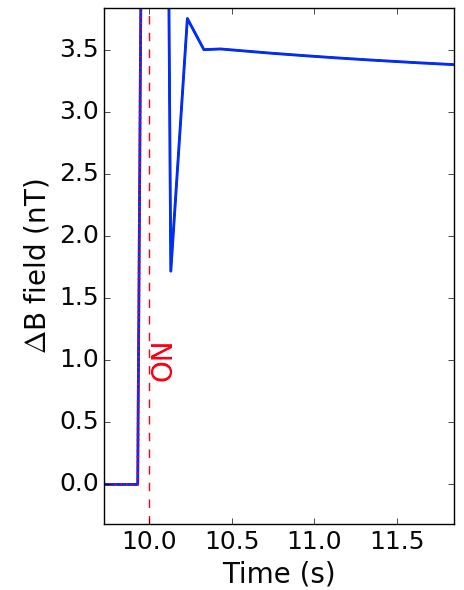
\includegraphics[width=\linewidth, height= 6.5 cm]{Images/i125_33_zoom.png}
%         \caption{at $k_c^i$=1.25}
%         \label{fig:i125zoom}
%     \end{subfigure}

%     \caption[short]{Zoomed in version of the drift $\Delta B$ shown in right side of Fig.~\ref{fig:i_pi}\textcolor{blue}{(a)}, Fig.~\ref{fig:i_pi}\textcolor{blue}{(b)}, Fig.~\ref{fig:i_pi}\textcolor{blue}{(c)} and Fig.~\ref{fig:i_pi}\textcolor{blue}{(d)} respectively at sensor position '1x' for different values of $k_c^i$ with $k_c^p$ ( see Eq.~(\ref{eq:I}) ) being zero. The red vertical dashed line indicates the time of the perturbation coil being turned 'ON'. For position of coils and sensors see Fig.~\ref{fig:coil}.\label{fig:i_pi_zoom}}
% \end{figure}

% \fig{Images/i_pi_zoom}{width = \textwidth,height =10cm}{Zoomed in version of the drift $\Delta B$ shown in right side of Fig.~\ref{fig:i_pi}\textcolor{blue}{(a)}, Fig.~\ref{fig:i_pi}\textcolor{blue}{(b)}, Fig.~\ref{fig:i_pi}\textcolor{blue}{(c)} and Fig.~\ref{fig:i_pi}\textcolor{blue}{(d)} respectively at sensor position '1x' for different values of $k_c^i$ with $k_c^p$ ( see Eq.~(\ref{eq:I}) ) being zero. The red vertical dashed line indicates the time of the perturbation coil being turned 'ON'. For position of coils and sensors see Fig.~\ref{fig:coil}.\label{fig:i_pi_zoom}}


%

The above results show that using only the I term provides better
compensation, but then it gives rise to slowly-varying currents that
take a long time to settle.  I often refer to this problem as the
``current drifting problem'' in the remainder of this thesis.

% \subsection{r vs. Condition No.}\label{sec:cond}
% Instead of going through all the steps that are discussed in Section~\ref{sec:inv}, the concept of condition number of a matrix can be used. The condition number of $\bm{M}$ can be determined from the diagonal matrix $\bm{\Sigma}$ as given in eq.\ref{eq:m} by -
%  \begin{equation}
%      cond(\bm{M})=\frac{max(\sigma_d)}{min(\sigma_d)}
%  \end{equation}
 

\subsection{Effect of adjusting both P and I}

In this section, I tuned the P and I terms following the
Ziegler-Nichols procedure (discussed in Section~\ref{sec:tune}). The
tuned values were found to be $k_c^p=0.60$ and $k_c^i=0.37$.

% \fig{Images/p60i368}{width = \textwidth,height=7cm}{Currents (left vertical axis) in all six coil sides ($C_x^\pm$, $C_y^\pm$ and $C_z^\pm$) with drift $\Delta B$ (right vertical axis) at 12 sensor positions with fluxgate positions 1, 3, 6 and 8 for $k_c^p$=0.6 and $k_c^i$=0.37 (see Eq.~(\ref{eq:I})). For position of coils and fluxgates see Fig.~\ref{fig:coil}. All grey color curves in $\Delta B$ graph denote the drift in signal that would have been without the compensation while all other color curves denote the actual drift in signal at fluxgate positions 1, 3, 6 and 8 found by Eq.~(\ref{eq:del_B}). Vertical dashed lines indicate the time of the perturbation coil being turned on and off. The current supplied on perturbation coil was 10  mA. The resolution index 1 (see Table~\ref{table:t7freq}) with 50 no of averages per measurement was used. The loop sampling frequency was found to be $\sim$6.5 Hz.\label{fig:tuned_vs_i}}{Coil currents with drift $\Delta B$ for $k_c^p$ and $k_c^i$ combined.}



% For simplicity instead of showing all the drift $\Delta B$ for all the fluxgate sensors for the positions given in the horizonatal axis of Fig.~\ref{fig:m}, only '1x' is shown on the right of the figure. And same as earlier the currents  that are being sent to the coils ($C_x^\pm$, $C_y^\pm$ and $C_z^\pm$) shown on the left of the same figure. But, we couldn't determine the effect of having both of them at a time. So, keeping $k_c^i$ as 0.52 and excluding P term i.e. $k_c^p$=0.0 we run the same measurement again and the results are shwon in Fig.~\ref{fig:tuned_vs_i}\textcolor{blue}{(b)}. As as matter of surprise, there is hardly any difference between the results in Fig.~\ref{fig:tuned_vs_i}\textcolor{blue}{(a)} and Fig.~\ref{fig:tuned_vs_i}\textcolor{blue}{(b)}. Why is that so ? For the moment, the Fig.~\ref{fig:tuned_vs_i} suggests that may be we don't need P term at all or maybe we need different tuning methods. So, applying P and I term at a time raises question of the necessity of the P term or importance of the tuning method describe in Section~\ref{sec:tune}. Due to lack of time, we did not further go into other tuning methods. Rather we have tried to discover the differences in the work between Ref.~\cite{bea} and Ref.~\cite{rawlik}.



\fig{Images/pi_i_mCond30}{width=\textwidth,height=12cm}{Currents (left) in all six coil sides with field measurements $\Delta B$ (right) from 12 sensor axes with fluxgate positions 1, 3, 6 and 8 for $k_c^i=0.37$ and adjusting (a) $k_c^p=0.6$ to (b) $k_c^p=0$.  Grey curves denote the uncompensated field change.\label{fig:pi_i_mCond30}}{Coil currents with drift $\Delta B$ for different values of $k_c^p$ only.}

The results of running the system with these parameters is shown in
Fig.~\ref{fig:pi_i_mCond30}\textcolor{blue}{(a)} It is seen that the
coil currents (left) and $\Delta B$ (right) graphs have similar pattern
to only I term pattern which is shown in
Fig.~\ref{fig:pi_i_mCond30}\textcolor{blue}{(b)} where only
$k_c^i$=0.37 is used.

% \fig{Images/mont_i}{width = \textwidth}{The effect of $k_c^i$ on current fluctuations (a) and remaining field fluctuations (b) for fluxgate positions 1, 2, and 7. Here, 100 mA current has been supplied in the perturbation coil and $k_c^p$=0.7 and $r$=3.5 have been used. For position of the fluxgates  and coil see Fig.~\ref{fig:coil}.\label{fig:mont_i}}{The effect of $k_c^i$ on fluctuations.}
% \doublefig{Images/p43i52_33}{width =\textwidth,height =8cm}{at $k_c^p$=0.43 and $k_c^i$=0.52. \label{fig:pi_tuned}}{Images/i52_33}{width = \textwidth,height =8cm}{at $k_c^p$=0.0 and $k_c^i$=0.52..\label{fig:i52}}{{Currents (left vertical axis) in all six coil sides ($C_x^\pm$, $C_y^\pm$ and $C_z^\pm$) with drift $\Delta B$ (right vertical axis) at sensor position '1x' for combine different values of $k_c^i$ and $k_c^p$ ( see Eq.~(\ref{eq:I}) ). Blue color curve denotes the actual drift in signal at position '1x' found by Eq.~(\ref{eq:del_B}), while the red curve denotes the drift that would have been without the compensation. Vertical dashed lines indicate the time of the perturbation coil being turned on and off. For position of coils and fluxgate sensor see Fig.~\ref{fig:coil}.} \label{fig:tuned_vs_i}}{short}

The conclusion is that the P term has a smaller effect compared to the
I term which is seen from comparing Fig.~\ref{fig:p_pi} with
Fig.~\ref{fig:i_pi} and Fig.~\ref{fig:pi_i_mCond30}.  It is also clear
that it is important to do some fine tuning of the PI parameters
beyond Ziegler-Nichols in order to get the best feedback results.

Unfortunately, neither applying Ziegler-Nichols nor doing any
additional tuning was able to change the current drifting problem.
Although it does not appear when only the P term is nonzero, this was
deemed undesirable because of proportional droop and the fact that the
compensation results for the magnetic field were clearly better when
using the I term or combined PI tuning.
% \item Do we need all the figures?  Can the data be summarized better (all currents and all fields on two graphs for each setting?)
% \item Should we show data?  I think so.  Need to establish that the simulation agrees with the data.  That could also be a major point of this section.  It would also lead into discussion of the current-drifting problem and that since the simulation and data agree, and we checked the hardware, that it is not a hardware problem..

\subsection{The ``Current Drifting Problem''}

Because of the current drifting problem, I changed a large number of
parameters in order to try to determine its cause.  For example, one
suspicion was that it could be due to malfunctioning power supplies
that were themselves drifting, but that the feedback loop was
stabilizing.  This was ruled out by careful tests of the power
supplies, and by running the system with a reduced number of axes of
control.  For example, when only one axis of control was used, the
system performed just like a usual PI loop with properly adjusted
currents and fields.  This is one reason the studies presented in
Section~\ref{sec:inv} were done.

Section~\ref{sec:flux_place} represents other studies that were geared
mostly at solving this problem.  In these studies the positioning of
the fluxgates were changed and the passive shield within the coils was
removed.  As will be shown, neither had an impact on the current
drifting problem.

In Section~\ref{sec:pSim}, simulation results are presented and
compared with the data.  It was at this point that we started to gain
confidence that this was a true problem of multidimensional control,
because, surprisingly (to us) the simulations agreed perfectly with
the data and even reproduced the current drifting problem.

By the studying the simulation results and the conditioning of the
matrix (Section~\ref{sec:cond}), we eventually determined that
ill conditioning was the main problem.  The next several sections all
follow this theme of developing a better understanding of
multidimensional control and ultimately show that the simulation tools
I developed are the best way to design the control system.


\section{Fluxgate Placements and Impact of Passive Shield}\label{sec:flux_place}

%\begin{itemize}
%\item We still had no clue so we just started changing things randomly.
%\item We changed fluxgate positions to try to make cond number smaller to see if it had an effect.  Could not change the cond number or the problem significantly.  (Table 5.1).  We also ran the compensation system and it still had the current drifting problem to varying degrees.
%\item We were confused if the slow current response might be due to magnetic responses that were slow.  So we tried removing the shields.  No change.  Fig. 5.9.
%\item And then we realized this had nothing to do with it.
%\end{itemize}

An observation of the previous section was that the coil current does
not settle properly although the field seems to be compensated on
shorter timescales than the settling time for the currents.  We called
this the ``current drifting problem'' as noted in the previous
Section.  I developed hypotheses to try to explain this observation
and then began to test these hypotheses experimentally.

The two hypotheses to explain the current drifting problem that are
addressed in this Section are:
\begin{enumerate}
\item The fluxgate positions might be affecting the measurement.   To address this, I adjusted the fluxgate positions to try to reduce the condition number and see if this had a positive effect.  I tried different positions mainly in
corners and center of each of the coil faces, and at various distances
inside and outside the coil cube.  The conclusion of this study was
that I could not change the condition number or the current drifting
problem significantly.
\item The slow current response might be due to magnetic responses that were slow.
To address this, I tried removing the magnetic shielding system from
the coil cube and re-tuning the system.  The conclusion of this study
was that it also did not fix the problem.
\end{enumerate}
In this Section, the results of those studies are shown and discussed.
As will be shown in Section~\ref{sec:coil_config}, the problem
originates from having too many degrees of freedom in the coil system
itself.  Nonetheless these studies are important to show the process
by which we learned this.

\subsection{Fluxgate Placements}

Previous work of others did not fully investigate the principles by
which the fluxgate positions should decided.  In general the strategy
of Ref.~\cite{bea} was to place a larger number of
fluxgates than required at conveniently mounted locations, generally
distributed within the region of the coils and magnetic shield.

Based on this reference, we started taking data with $14\times 3$-axis fluxgate
magnetometers placed just inside various corners of our coil cube.
One hypotheses was that increasing the number of sensors would
eliminate the problem of current drifting. To test this, we
implemented additional fluxgate sensors and build an additional
breakout box (see Section~\ref{sec:sensor}) so that we could acquire
magnetic field data from them.  This still gave anomalously slow
responses in the coil currents.

Another hypothesis was that placing the magnetometers at the center of
each of the faces of the coils could improve the current response, or
that more generally a broader range of positions should be tried.  A
general finding was that this also had not much effect on reducing the
condition number significantly, nor did it have an effect on the
current drifting problem.

\begin{table}%[htb!]
    \centering
    \begin{tabular} { |c|c|c|c|c|c|} 
        \hline
        \makecell{Fluxgates \\Position} & \makecell{$\bm{M}$\\ Condition No.} &\makecell{$\bm{M^{-1}}$\\ Condition No.} & $r$ & $r'$\\
        \hline\hline
        1, 3, 6 and 8 & 33.25 & 2.63 & 2.97 & 2.95\\ 
        \hline
        2, 4, 5 and 7 & 28.55 & 1.98 & 3.04 & 3.06 \\ 
        \hline
        \makecell{Center \\($C_x^\pm$, $C_y^\pm$ and $C_z^\pm$)} & 36.24 & 1.8 & 2.47 & 2.49 \\ 
        \hline
        \makecell{Center-6cm \\($C_x^\pm$, $C_y^\pm$ and $C_z^\pm$)} & 98.61 & 3.05 & 2.36 & 2.34 \\ 
        \hline
        \makecell{Center+6cm \\($C_x^\pm$, $C_y^\pm$ and $C_z^\pm$)} & 80.74 & 1.49 & 2.26 & 2.02 \\ 
        \hline
        \makecell{1, 2, 3, 4, \\5, 6, 7 and 8} & 28.30 & 1.94 & 3.17 & 3.19 \\ 
        \hline
        \makecell{1, 2, 3, 4, \\5, 6, 7, 8 and \\Center ($C_x^\pm$, $C_y^\pm$ and $C_z^\pm$)}  & 21.84 & 1.8 & 3.23 & 3.37 \\ 
        \hline

    \end{tabular}\caption[Matrix properties for different numbers of
   fluxgate sensors at different positions.]{Matrix properties for
   different numbers of fluxgate sensors at different positions.  The
   nomenclature for the positions of the fluxgates is explained in
   Fig.~\ref{fig:coil}.  The column $r$ represents the regularization
   method which is explained in Section~\ref{sec:mont} and $r'$
   represents the regularization method which will be explained in
   Section~\ref{sec:cond}.}\label{table:flux-pos}
\end{table}

The results for condition number are summarized for a representative
subset of these tests in Table~\ref{table:flux-pos}.  Both the
condition number of the matrix (equivalent to the condition number of
the unregularized pseudoinverse) and the condition number of the
regularized pseudoinverse are reported.  Two very similar
regularization parameters $r$ and $r'$ are reported.  The
regularization parameter $r'$ was determined by a new method I
developed and the method will be discussed further in
Section~\ref{sec:cond}.

The positions of the fluxgates are defined by the numbers for corner
positions (see Fig.~\ref{fig:coil}) and when they are in the center of
each of the coil faces they are termed as Center ($C_x^\pm$, $C_y^\pm$, and
$C_z^\pm$). Center-6cm means all the sensors in the center of the coil
faces have been brought 6~cm towards the origin at the center and
Center+6cm means they are 6~cm farther away from the center.

The matrix can be created for an arbitrary number of sensor positions
by moving the sensors and recording field data for the various coil
settings in subsequent runs.  This has been done for example in the
lowest row of the table where $14\times 3$-axis fluxgates have been
incorporated into the matrix.

The general conclusion of Table~\ref{table:flux-pos} is that while the
fluxgate positions have some impact on the condition number of both
the unregularized and regularized pseudoinverse, they do not solve the
problem of ill-conditioning: the matrix must still be regularized or
the current fluctuations driven by the compensation system would be
unacceptably large.  Even with significant changes in the fluxgate
positions ({\it e.g.}~corners vs.~center faces) the condition number
changes at most by a factor of three in the unregularized
pseudoinverse and a factor of $<2$ for the regularized pseudoinverse.
Interestingly, even if a large number of sensors are included ({\it
e.g.}~the final two rows of the table), this does not necessarily have
a positive impact on the condition number.

Another conclusion is that an over-constrained system (more fluxgate
axes than coils) is not necessarily sufficient in order to have a
well-conditioned problem.  It is not even clear whether an
over-constrained system is absolutely necessary to generate good
control.  For example, at the center face positions, the fluxgates
only ever sense a large magnetic field in one particular direction,
because the magnetic field must be perpendicular to the magnetic
shield at this point.  It effectively reduces the number of fluxgate
axes to six, which is equal to the number of coils being used for
control.  And yet this gives an almost the same ill-conditioned
properties for the matrix as any other row in the Table.  We also
tried studies where we used only those six axes in the control system,
with very similar results to the corner-placement positions.

In Section~\ref{sec:pSim}, I will report a simulation which is
successful in reproducing these results.  Although not shown here, the
results of PI tuning of the systems for which we had enough sensors
were also acquired.  None of the positions gave particularly better PI
control than any of the others and all of them generally suffered from
the same current drifting problem.

I also tried slight adjustments to the corner positions and this had a
similar small effect.  It will be discussed further in
Section~\ref{sec:cond} that it is also noticeable that regularization
by two different methods (the method of Ref.~\cite{bea}
and my new method) agree.

% \doublefig{Images/cB_t_center_p}{width =\textwidth, height= 6 cm}{Position=1,2,3,4,6,8\label{fig:cb_center_p}}{Images/cB_t_center_pi}{width = \textwidth, height= 6 cm}{Position=1,2,3,4,6,8\label{fig:cb_center_pi}}{{PI Active Magnetic Field Compensation Results by both Experiment and Simulation.} \label{fig:cb_center}}

% \doublefig{Images/bt6}{width =\textwidth, height= 7 cm}{Position=1,2,3,4,6,8\label{fig:bt6}}{Images/sf6}{width = \textwidth, height= 7 cm}{Position=1,2,3,4,6,8\label{fig:sf6}}{{PI Active Magnetic Field Compensation Results by both Experiment and Simulation.} \label{fig:btSF6}}

% \doublefig{Images/bt8}{width =\textwidth, height= 7 cm}{Position=1,2,3,4,5,6,7,8\label{fig:bt8}}{Images/sf8}{width = \textwidth, height= 7 cm}{Position=1,2,3,4,5,6,7,8\label{fig:sf8}}{{PI Active Magnetic Field Compensation Results by both Experiment and Simulation.} \label{fig:btSF8}}

%The above discussion of the Table~\ref{table:flux-pos} shows that
%current goes crazy if the fluxgates are placed in the center of each
%of the coil faces and crazier if they are slightly moved inside or
%outside of the center. The corners position fluxgates shows normal
%behaviour compare to the center positions. But the study does not help
%us solving our original problem of slow current response.

% To quantify more we have taken the help of regenerating Fig.~\ref{fig:Isim} and Fig.~\ref{fig:fluc-sim}. From Fig.~\ref{fig:Isim}, we have recorded the maximum  $\Delta I_c^{\text{simRMS}}$ (mA) for 30 different sets of $B_s^{\text{rand}}$. For maximum compensation we have generated the Fig.\ref{fig:fluc-sim} for same for 30 different sets of $B_s^{\text{rand}}$ from which we have recorded lowest the remaining fluctuation F. For example- for fluxgate positions 1, 3, 6 and 8, the lowest F goes to 0.3. That means the maximum compensation due to the field produced by $\Delta I_c^{\text{sim}}$to counteract $B_s^{\text{rand}}$ is(1-0.3$\times$100$\%$) =70$\%$. For more details see Section~\ref{sec:mont}. It seen that the current goes crazy if the fluxgates are placed in the center of the coil faces and the maximum $\Delta I_c^{\text{simRMS}}$ ranges from 98 to 192 mA. But the maximum $\Delta I_c^{\text{simRMS}}$ is 12 mA when the center fluxgates are used with the corners one. But on that time the maximum compensation due to the field produced by $\Delta I_c^{\text{sim}}$to counteract $B_s^{\text{rand}}$ is only 15$\%$. So, anything with center seems to give crazy results. Then by looking at the all the three parameters e.g. matrix condition number, maximum $\Delta I_c^{\text{simRMS}}$ and maximum compensation for the 3 different sets of corner positions only, it is seen that the results are more balanced and surprisingly the compensation with 4*3-axis sensors are better than 8*3-axis sensors in exchange of more maximum $\Delta I_c^{\text{simRMS}}$.





% The increase in matrix condition number for the center of the coil sides is noteworthy.  So, a study has been done to see the current response effect while sensors are in the middle of the coil sides as shown in Fig.~\ref{fig:cb_center}. The Fig.~\ref{fig:cb_center_p} represents the current response on all the six coil sides with their effect on the $z$-axis in the origin as shown in the right with only choosing proportional (P) term. But just adding a small fraction of integral resest (I) term makes the current response unstable as shown in Fig.~\ref{fig:cb_center_pi}. So only P controller is suitable if fluxgates are placed in the middle of the coil sides but in the case of corner positions either P only or I only or PI controller option is available. In a summary, the more the sensors the more is the matrix condition number. Corner positions are better in terms of different freedom of controlling.

% \doublefig{Images/cB_t_center_p}{width =\textwidth, height= 6 cm}{Position=1,2,3,4,6,8\label{fig:cb_center_p}}{Images/cB_t_center_pi}{width = \textwidth, height= 6 cm}{Position=1,2,3,4,6,8\label{fig:cb_center_pi}}{{PI Active Magnetic Field Compensation Results by both Experiment and Simulation.} \label{fig:cb_center}}

% \doublefig{Images/bt6}{width =\textwidth, height= 7 cm}{Position=1,2,3,4,6,8\label{fig:bt6}}{Images/sf6}{width = \textwidth, height= 7 cm}{Position=1,2,3,4,6,8\label{fig:sf6}}{{PI Active Magnetic Field Compensation Results by both Experiment and Simulation.} \label{fig:btSF6}}

% \doublefig{Images/bt8}{width =\textwidth, height= 7 cm}{Position=1,2,3,4,5,6,7,8\label{fig:bt8}}{Images/sf8}{width = \textwidth, height= 7 cm}{Position=1,2,3,4,5,6,7,8\label{fig:sf8}}{{PI Active Magnetic Field Compensation Results by both Experiment and Simulation.} \label{fig:btSF8}}
% The above discussion of the Table~\ref{table:flux-pos} shows that current goes crazy if the fluxgates are placed in the center of each of the coil faces and crazier if they are slightly moved inside or outside of the center. The corners position fluxgates shows normal behaviour compare to the center positions and surprisingly less sensors shows better compensation in the corners in exchange more more currents.


\subsection{Impact of Passive Shield}

Fluxgate placements failed to solve the slow coil current response.
Another hypothesis developed around this time was that increasing
sampling frequency will solve the problem.  So, besides the advantages
discussed in Section~\ref{sec:freq}, solving the slow current response
time was also a motivation to build the filters as that would allow us
to use the fastest sampling frequency of the ADC.  As can be seen in
that Section, using the filter, we successfully reduced the response
time but still suffered from current drifts over long timescales.

Then we thought the passive shielding layer might have cause some
slower response of the system, perhaps due to slow changes in the
magnetization of the shield. To test if this affected the feedback and
control system, I conducted tests where I removed the magnetic shield
from within the coil cube.


% After that we decided to use the fastest sampling frequency of our ADC for which we have to build the filters.  Now, due to this the current response time has increased but that was not the solution of the current unsettle problem. Finally, we have realized that in addition to fastest response we have to also consider the matrix condition number and if the condition number is large then we have to lower the value of optimized $r$ (see Section~\ref{sec:new_study_r}). Here, we will talk about the the studies we have done on fluxgate placements.
\fig{Images/shield_noShield}{width=\textwidth,height=12cm}{Magnetic compensation results (a) with shield and (b) without shield within the coil cube.  The fluxgate positions are 1, 3, 6 and 8.  The feedback and regularization parameters are $k_c^p=0.0$, $k_c^i=1.0$, and $r=2.8$.  The current supplied to the perturbation coil was 25  mA when switch on. Resolution index 1 with 50 averages per cycle were used.\label{fig:shield_noShield}}{Comparison of magnetic compensation results with and without the magnetic shield present.}

Fig.~\ref{fig:shield_noShield} compares the response of the system
with the outermost magnetic shield layer inside the coil cube, to the
response when no magnetic shields are present within the coil cube.  When the
shield is removed, it changes the matrix elements significantly. The
matrix was therefore remeasured and the regularization process redone.
It was possible to get satisfactory results for the inversion of both
matrices (shield and no shield) using $r=2.8$.
Fig.~\ref{fig:shield_noShield} demonstrates that removal of the
magnetic shield, while having a significant impact on the matrix
elements, does not have much impact on the effectiveness of the system
to compensate the field.  It also has no impact on the current
drifting problem, although the pattern of currents has changed
somewhat, because of the change in the matrix elements.

Another difference between Fig.~\ref{fig:shield_noShield} and
Fig.~\ref{fig:i_pi} is that the connection of the coils to current
sinks was changed, resulting in a change in the sign of some of the
currents.  These kinds of changes were also done often in order to try
to address the current drifting problem and conduct tests of the
current sinks.


% except for the case of shield, the matrix condition number is less. The Fig.~\ref{fig:btSF8_s} shows the AMC compensation (Fig.~\ref{fig:bt8_s}) and the corresponding allan deviation and shielding factor ( Fig.~\ref{fig:sf8_s}) with outermost layer of shield. The matrix condition number is found to be 19. Similarly, the Fig.~\ref{fig:btSF8} shows the AMC compensation (Fig.~\ref{fig:bt8}) and the corresponding allan deviation and shielding factor ( Fig.~\ref{fig:sf8}) without any shield. The matrix condition number in this case is 132. The one advantage of having shielding is that , the shielding factor for all the sensors remain $geq$1 but in case of no shield, the shielding factor may be very good at certain point but in some point it can go below 1.



% \doublefig{Images/bt8_shield}{width =\textwidth, height= 7 cm}{Position=1,2,3,4,6,8\label{fig:bt8_s}}{Images/sf8_shield}{width = \textwidth, height= 7 cm}{Position=1,2,3,4,6,8\label{fig:sf8_s}}{{Shield} \label{fig:btSF8_s}}{short}

% \doublefig{Images/bt8}{width =\textwidth, height= 7 cm}{Position=1,2,3,4,5,6,7,8\label{fig:bt8}}{Images/sf8}{width = \textwidth, height= 7 cm}{Position=1,2,3,4,5,6,7,8\label{fig:sf8}}{{No SHield} \label{fig:btSF8}}{short}

In the end, neither fluxgate placement nor shielding effect provided a
solution of the current drifting problem.  How I really started to
determine the source of the problem was by simulating the full,
multidimensional feedback and control system.

\section{Simulation of Multidimensional Feedback System}\label{sec:pSim}

I developed a variety of simulation tools in order to understand the
behavior of the multidimensional PI control loop:
\begin{enumerate}
\item {\bf Three-dimensional finite-element analysis simulations in OPERA.}  These were used to simulate
\begin{enumerate}
\item the quasi-static magnetic response of the magnetic shield to Earth's field
\item the magnetic response of the magnetic shield to changes in coil-cube currents (in turn enabling us to determine $\bm{M}$), and
\item the magnetic response of the magnetic shield to the perturbation coil (in turn allowing us to simulate the PI system response to this pertubation.
\end{enumerate}
\item {\bf Field Map Processing in Python.}  The OPERA simulations provided full three-dimensional field maps.  Python scripts were written to process and simplify the information into {\it e.g.}~the matrix $\bm{M}$, or the changes seen at each fluxgate position when the perturbation coil was energized.
\item {\bf PI Simulation in Python.}  With this reduced information in hand, the full PI loop was also simulated in Python in real time.  This allowed me to simulate the full time-dependent response of the feedback and control system to the perturbation coil.
\end{enumerate}
As will be shown, these simulations were quite successful at
describing the system including: the matrix $\bm{M}$ and its
inverse, and the time-dependent response of the PI loop to
perturbation.

\subsection{Simulation in OPERA to Generate Field Maps in Coil Cube}
% The simulating process will be discussed here at first and then the result of the simulation will be compared with the experiment and whether there is current unsettle problem exists in the simulation will be discovered.

OPERA 3D Finite Element Analysis~(FEA)~\cite{opera} simulation
software was used for simulating the prototype and generating field
maps within the coil cube of the prototype. OPERA is a multi-physics
software package.  We have used the Opera Static Electromagnetics
module which computes magnetostatic and electrostatic fields in three
dimensions. The module solves Maxwell's equations for the static case
in a discretized model using FEA. For calculating magnetic fields from
coils, the module uses the Biot-Savart integral equation.

%\begin{itemize}
%    \item define the geometry of the experimental setup.
%    \item extract the magnetic field values within the geometry.
%    \item energize each coil.
%\end{itemize}



% which allows coupled simulations including the ability to couple a Static Module simulation with a thermal simulation or a stress simulation, for example to calculate the stress due to electromagnetic forces.The module automatically switches to the part containing magnetic sources in case of magnetostatics.or direct current (DC) flow .To calculate the potential at each node of the mesh, OPERA uses an iterative solution technique which is memory-efficient and computationally fast. In this module, the properties of the magnetic materials can be specified as required i.e. linear, non-linear, isotropic, anisotropic, laminated or permanent magnet. 



% and then move forward to all the simulations made to run a fully functional PI simulation. For, data analysis, sorting  and modifying the data and also running the PI control algorithm the Python programming language has been used alongside the simulation software. The complete simulation is made of three different simulations. 

% \begin{itemize}
%     \item Making geometry of the experimental setup and extracting the magnetic field values in that geometry
%     \item Simulation of Matrix M
%     \item Simulation of Magnetic Field Distribution
%     \item Simulation of PI Control
% \end{itemize}
% In the following  all of the above simulations  will be discussed in detail starting with the simulation software itself. The section ends with comparing the simulation results with the experimental ones.

% \subsection{About Simulation Software}
% Here, the simulation software has been discussed in detail. Mainly, the focus is on the the module of the software that we have used .



% In the upcoming Sub-sections, the geometry that has been built will be discussed along with all the steps done to finally make a PI control simulation.


\subsubsection{Geometry Definition in OPERA}

\doublefig{Images/shield2}{width=\textwidth,height=8cm}{\label{fig:shield_opera}}{Images/noShield}{width=\textwidth,height=8cm}{\label{fig:noShield_opera}}{{Geometry in OPERA simulation (a) with passive shielding, and (b) without passive shielding.  The square in the back, appearing in both drawings, is the perturbation coil. The direction of each of the three axes may be seen in (b).} \label{fig:opera_setup}}{Prototype geometry in OPERA simulation}

Fig.~\ref{fig:opera_setup} shows the geometry as defined in OPERA,
both with and without the magnetic shields present.  The dimensions of
the prototype passive shielding layers and the stove pipe were given
in Table~\ref{table:mu-metal}.  These were implemented using simple
cylindrical and planar shapes available in OPERA.  The dimensions of
the coils were given in Table~\ref{table:coil}.  These were
implemented as wires of square profile 1.24~m~$\times$~1.24~cm.

The material of the magnetic shield was chosen to be linear with
relative magnetic permeability $\mu_r=20,000$.  Some air volumes were
also drawn near the shields to aid in meshing near the thin layers.

The perturbation coil is 1.06~m away from the origin, which is at the
center of the coil cube.

All the information has been written in the {\tt comi} file format
file which is the command language in OPERA. Another {\tt comi} file
was made with no shield
(Fig.~\ref{fig:opera_setup}\textcolor{blue}{(b)}) for simulation of
that experiment.  The dots in
Fig.~\ref{fig:opera_setup}\textcolor{blue}{(b)} represent some
fluxgate positions.  But in general both simulations outputted full
field maps so that the fluxgate positions could be adjusted
arbitrarily after the simulation was complete.

A cubic mother volume with side length 4 times the side length of the
coil cube was used.

%{\bf consider a Table for the following paragraph.}

\fig{Images/surface_mesh}{width =0.8\textwidth}{Settings to generate surface mesh in OPERA. \label{fig:s_mesh}}{Settings to generate surface mesh in OPERA.}

In OPERA, surfaces are first meshed, and then these meshes are
extended into the volume with a subsequent volume meshing step.
%\textcolor{red}{To
%generate the surface mesh, the maximum mesh element size was chosen to
%be 10 with maximum angle between elements of 10$^\circ$. The maximum
%deviation from surface was set to 0 and the absolute tolerance used to
%check point coincidence was set to $1\times10^{-8}$. The mesh
%type was set to ``Prefer Mosaic''.}
The settings used to generate the surface mesh are presented in
Fig.~\ref{fig:s_mesh}, where a portion of the settings window is
shown.  To generate the volume mesh there is one additional setting
which is another absolute tolerance; it was set to $1\times10^{-8}$.

\subsubsection{Simulation Applying Current in Compensation Coils}\label{sec:mSim}

%In Section~\ref{sec:m}, matrix elements $M_{sc}$ are measured  to produce $\bm{M}$ which relates coil currents with the magnetic field. Inversion of the matrix produce current error (Eq.~(\ref{eq:del_I})) that later goes to PI control algorithm (Eq.~(\ref{eq:I})) to find new current that should be fed to compensate the drift in field. For matrix simulation, zero magnetic field is applied so that six current generated field map in T/A for six coils in the cube can be generated with current being supplied to the the coils one at a time with others having zero current. The process is discussed here. 

In order to simulate the matrix $\bm{M}$ we need to energize each
coil in turn and measure the magnetic field change at each fluxgate
position.

In OPERA, a coil was energized by setting its current density to
1~A/area, where the area is determined automatically by the OPERA
based on the dimensions provided.  To conduct the finite element
analysis, I used the TOSCA magnetostatic module of OPERA.  I set the
numerical solution convergence tolerance to be $1\times10^{-13}$.

Once the solution for a single energize coil was completed, the field
map was outputted to a file using the the post-processor of OPERA.
The unit of the magnetic field was set to be T, and I used the GRID
command which evaluates the fields over a uniform 3D grid. The grid
started from $-62$~cm in $x$, $y$ and $z$ co-ordinates with an
increment of 1~cm and ends at $+62$~cm which covers the full cube
dimensions.  The output of the GRID command gives a text ({\tt csv})
file with 6 columns, where the first 3 columns indicate the
coordinates of the grid point ($x$,$y$,$z$) and the last 3 columns
indicate the magnetic field ($B_x$,$B_y$,$B_z$) at that point.  In
this way 6 field maps are stored in 6 {\tt csv} files, one for each of
the 6 coils.

% The background region defines the sa 'comi' file is written where the magnetic field contribution due to environment is set to zero as  matrix elements $M_{sc}$ relate the coils current to the field produced by the coils current (see Eq.~(\ref{eq:B_coils})). Now as matrix elements $M_{sc}$ are in the unit of nT/A, in the same 'comi' file current for the all the six coils have set to 1A which makes the Eq.~(\ref{eq:B_coils}) as

% \begin{equation}\label{eq:B_coils_1A}
%     B_s(\text{coils})=\sum_c^{c=1-6} M_{sc}
% \end{equation}
% where, $n$=1.

% Now the 'comi' file for the above setup will interact with the 'comi' file of the prototype geometry and then by using the solver of OPERA, $B_s(\text{coils})$ i.e. $M_{sc}$ elements will be calculated.

% \renewcommand{\labelitemi}{$\blacksquare$}
% \begin{itemize}
%     \item[$\blacksquare$] \textbf{Creation of Matrix M}
% \end{itemize}

% The advantage of simulation is that we have got 6 field maps for 6 coil sides which we can use to generate any dimensions of matrix $\bm{M}$ within the cube dimensions. For generating the matrix, we used the Python programming language where the fields maps are acted as input. We convert the fields maps into nT/A and depending on the co-ordinates of the points provided by us, the matrix is generated in the output of the Python code. Note that the points must be from -62 cm to 62 cm with an increment of 1 cm in each of the $x$, $y$ and $z$ co-ordinate.


% % The best thing about simulating in this setting is that the OPERA has calculated the $M_{sc}$ elements for the whole volume of the prototype geometry which can be easily exported in a 'csv' file by running a simple 'comi' file for volume extraction. Thus the $M_{sc}$ elements of the whole prototype geometry have been stored in a 'csv' file in T/A. Then, a code has been written in the Python programming language to clean, modify and sort the data of that 'csv' file and convert the data in nT/A and  provide the co-ordinates of the points from where the magnetic field values i.e.  $M_{sc}$ elements (see Eq.~(\ref{eq:B_coils_1A})) are determined.

% % And the current in the coils are related to the magnetic filed with those $M_{sc}$ elements as given in Eq.~(\ref{eq:B_coils}). It is very easy to extract magnetic field information by providing the co-ordinates vale in OPERA. In addition to the field produced by the coil currents, there is also  values of $M_{sc}$. That means, setting current, I=1 A and offset =0 in all six coil will produce 
% % \fig{Images/noShield}{width =\textwidth,height=14 cm}{Prototype setup in OPERA simulation software without passive shielding layers. \label{fig:noShield_opera}}

% For comparison with the experimental $\bm{M}$, the simulation $\bm{M}$ has been made by choosing co-ordinates of the points as same as the sensor positions in the experiment. Then the absolute differences between the experimental $M_{sc}$ elements with that of the simulation ones  are calculated as

% \begin{equation}
%     |M_{sc}^{\text{diff}}|=|(|M_{sc}^{\text{exp}}|-|M_{sc}^{\text{sim}}|)|
% \end{equation}
% where, $|M_{sc}^{\text{exp}}|$ and $|M_{sc}^{\text{sim}}|$ indicate the absolute values of $M_{sc}$ elements both in experiment and simulation respectively.
% The absolute differences $|M_{sc}^{\text{diff}}|$ have been shown in Fig. \ref{fig:Mdiff}. It is seen that most of $|M_{sc}^{\text{diff}}|$ differences are within 100 nT/A. But that in some of the positions the differences are very big. The reason is that it is very difficult to exactly pinpoint the locations both in experiment and simulation and also the simulation runs in ideal conditions where the experiment suffers from the condition of its surrounding. The differences can be made smaller by choosing different co-ordinates of the sensor positions. We are not that concerned about that because the $M_{sc}$ element due to a particular coil and sensor position has similar response pattern both in experiment and simulation. 

% \fig{Images/Mdiff_56}{width = \textwidth}{The absolute differences between the  experimental $M_{sc}$ elements with that of simulation in nT/A. Horizontal axis indicates the various sensors, which are counted using the index $s$. Vertical axis indicates the various coils, which are counted using the index $c$. The value of the elements are increasing from dark blue to red. For position of the sensors and coils please see Fig.~\ref{fig:coil}. \label{fig:Mdiff}}{Comparison of experimental $\bm{M}$ with simulation one.}

% 
% So, we have made simulation which can produce $M_{sc}$ elements for any number of the sensors placed in the prototype geometry. This will be a tool for the future students who are limited by sensor position and placing them correctly in their system to study in detail about the effect of $\bm{M}$ for any set of sensors.


% \subsection{Simulation of Magnetic Field Distribution}\label{sec:pSim}

% The main aim of active compensation is to compensate the drift that generates due to the difference between the setpoint and the actual measurement. The measurement of the field by fluxgates surrounding the prototype without any compensation system running are given in Table~\ref{table:Benvironment} which we have used to generate two field maps one with no current in any coils and another with current in the perturbation coil. The concept is that without any perturbation, the field is always same. So, the field map with no current in any coil will generate the setpoint i.e. $B_s(\text{setpoint})$ and the field map with current in perturbation coilwill generate the actual measurement i.e. $B_s(\text{measure})$. The difference between $B_s(\text{measure})$ and $B_s(\text{setpoint})$ will generate drift in field (Eq.~(\ref{eq:del_B})).

% and lastly how the perturbation affects the current in all six coil sides will be discussed. 

\subsubsection{The Effect of Earth's Field and of the Perturbation Coil}

The field maps of the previous section were calculated in the absence
of Earth's field.  In general, the fluxgate setpoints were decided by
first measuring the field and then selecting the setpoint based on
that measurement.  The feedback system would then try to lock the
fields to those setpoints.

The average field measured by fluxgates surrounding the prototype
without any compensation system running were given in
Table~\ref{table:Benvironment}.  I used this information to try to
simulate the setpoints.  This was done for two field maps: one with no
current in any coils and another with current only in the perturbation
coil.  So, the field map with no current in any coil will generate the
setpoint i.e. $B_s(\text{setpoint})$ and the field map with current in
perturbation coil will generate the actual measurement
i.e. $B_s(\text{measure})$. The difference between
$B_s(\text{measure})$ and $B_s(\text{setpoint})$ will generate the
change in field $\Delta B$.

The six field maps generated by the coil-cube simulation of the
previous section can be added to these maps without loss of generality
under the assumption of linear material properties.

% The magnetic field distribution without any current in the coils that is $B_s(\text{setpoint})$ will be determined by simulating the prototype in OPERA.
% The 770 mA is same as providing 10 mA in the experimental perturbation coil as the experimental one has 77 turns
We used the same meshing as described earlier.  The perturbation coil
was energized, or left unenergized, in a similar fashion as used for
the coil-cube.  
%\textcolor{red}{The main difference compared to the previous coil-cube simulati%on was
%that the magnetic field $\bm{H}$ on the boundary of the mother volume
%was set according to Table~\ref{table:Benvironment}}.
%\textcolor{blue}{
The main difference compared to the previous coil-cube simulation was
that the external magnetic field $\bm{H}$ on TOSCA analysis module was
set according to Table~\ref{table:Benvironment}.
%}
%\textcolor{magenta}{It is sometimes convenient to introduce a “background” magnetic field into
%an analysis. OPERA-3d supports this facility in magnetostatic TOSCA,
%ELEKTRA and CARMEN analyses and in SCALA. A uniform field with
%any orientation may be specified. In these analyses, the applied magnetic field contributes to the overall coil
%fields in the problem. It is equivalent to having an infinite solenoid whose
%axis is oriented in the direction of the field. Consequently, it is necessary
%for the exterior of the model space (the outer layers of finite elements in the
%mesh) to use reduced magnetic scalar potential. The extent of this layer is
%unimportant – a single layer of elements works just as well as making all
%the air reduced potential. }
Otherwise the
field was solved and outputted to a {\tt csv} file as in the previous
section.  Two {\tt csv} files (one each for the perturbation coil
switched on and off) were created.

% For generating setpoints, we have used the Python programming language where the fields map is acted as input. We convert the fields maps into nT as to match the experimental unit  and depending on the co-ordinates of the points provided by us, the $B_s(\text{setpoint})$ are generated in the output of the Python code. Note that the points must be from -62 cm to 62 cm with an increment of 1 cm in each of the $x$, $y$ and $z$ co-ordinate.

% While comparing experimentally measured setpoints with that determined by simulation we have found that, the values of Bx, By and Bz are differ by $\sim$2000 nT but they have the same signs with same order of magnitude in $x$, $y$ and $z$ co-ordinate. The different values can be due to not match the coordinate points exactly. 


% As long as the signs of Bx, By and Bz are same both in simulation and experiment, the difference is no issues as the main aim is to find the drift in the magnetic field.

%\subsubsection{Simulation of Field Map With Current in Perturbation Coil}

When the perturbation coil was switched on, its current density on the
was set to 770~mA/area.  The reason is that, in the experiment, 10~mA
current was normally provided to the perturbation coil which has
77~turns.

% \begin{itemize}
%     \item[$\blacksquare$] \textbf{Creation of Measurements}
% \end{itemize}

% For generating measurements, we have used the Python programming language where the fields map is acted as input. We convert the fields maps into nT as to match the experimental unit  and depending on the co-ordinates of the points provided by us, the measurements $B_s(\text{measure})$ are generated in the output of the Python code. Note that the points must be from -62 cm to 62 cm with an increment of 1 cm in each of the $x$, $y$ and $z$ co-ordinate.

% For comparing the simulation result with experimental one, the effect of the perturbation has been found in terms of change in the coil currents in all six coils both in simulation and experiment. For the simulation, in the above, $B_s(\text{setpoint})$ and $B_s(\text{measure})$ have been determined by choosing co-ordinates of the points as same as the sensor positions in the experiment from which the change in the signal i.e. $\Delta B_s$ have been determined using Eq.~(\ref{eq:del_B}). Finally, the change in the coils current i.e. the errors in the coils have been determined by multiplying $\Delta B_s$ with regularized pseudo-inverse of $\bm{M(\text{sim})}$ obtained from Section~\ref{sec:mSim} (see Eq.~(\ref{eq:del_I}) and Section~\ref{sec:inv}). For experiment the changes in the fluxgate signals are determined by applying 10 mA in the perturbation  coil and then find $\Delta B_s$ using Eq.~(\ref{eq:del_B}) and eventually find the change in coil currents in the same way as done for the simulation. The change in current in all six coil sides found due to experiment and simulation are given in Table~\ref{table:currentChange} where the simulation results are quite similar to the experimental ones for all six coils sides.

% \begin{table} [htb!]
%     \centering
%     \begin{tabular} { |c|c|c|c|c|c|} 
%         \hline
%         Coils & \makecell{Change in Current (mA)\\Experiment} & \makecell{Change in Current (mA)\\Simulation}\\
%         \hline\hline
%         $C_x^-$ & -26 & -32 \\ 
%         \hline
%         $C_x^+$ & 22 & 20 \\
%         \hline
%         $C_y^-$ & -30 & -24 \\
%         \hline
%         $C_y^+$ & 24 & 17 \\
%         \hline
%         $C_z^-$ & -14 & -13 \\
%         \hline
%         $C_z^+$ & 54 & 46 \\
%         \hline

%     \end{tabular}
%     % \vspace{4mm}
%     \caption[Comparison of change in current in experiment and simulation.]{Comparison of change in current in different coil sides at the time of applying perturbation both in experiment and simulation.}\label{table:currentChange}
% \end{table}

% 
% In the above, simulation made via OPERA to find $B_s(\text{setpoint})$ and $B_s(\text{measure})$ have been used to find the change in current in all six coil sides and matched with experimental results. 

%In the upcoming Section the field maps obtained due to various simulations in OPERA will be used to generate matrix and drift in signals which will then integrate in PI control algorithm to make a fully functional PI simulation.
% The values obtained due to this have been compared with the values due to experimental setup and the results are similar as shown in Fig. \ref{fig:noShield_cSim}.

% \fig{Images/cSim}{width =\textwidth, height=12cm}{Comparison of change in current in different Coil sides at the time of applying perturbation both in experiment and simulation. \label{fig:noShield_cSim}}

\subsection{Field Map Processing in Python}

A set of Python codes are used to generate files containing the matrix
$\bm{M}$ and $\Delta B$ perturbations from the OPERA field maps.
The codes accept as input the field maps and the coordinates for the
fluxgate positions, and then output the relevant field values from
OPERA.


%\subsubsection{$\bm{M}$ Matrix Comparison to Data}

%There are 6 field maps generated for currents in all six coils where
%each of the six field maps represents the values associated with the
%current bearing coil.  The advantage of simulation is that which we
%can use 6 field maps to generate any dimensions of matrix $\bm{M}$
%within the cube dimensions. For generating the matrix, we used the
%Python programming language where the fields maps are acted as
%input. We convert the fields maps into nT/A to match the experimental
%unit and depending on the co-ordinates of the points provided by us,
%the matrix is generated in the output of the Python code. Note that
%the points must be from -62 cm to 62 cm with an increment of 1 cm in
%each of the $x$, $y$ and $z$ co-ordinate.


% The best thing about simulating in this setting is that the OPERA has calculated the $M_{sc}$ elements for the whole volume of the prototype geometry which can be easily exported in a 'csv' file by running a simple 'comi' file for volume extraction. Thus the $M_{sc}$ elements of the whole prototype geometry have been stored in a 'csv' file in T/A. Then, a code has been written in the Python programming language to clean, modify and sort the data of that 'csv' file and convert the data in nT/A and  provide the co-ordinates of the points from where the magnetic field values i.e.  $M_{sc}$ elements (see Eq.~(\ref{eq:B_coils_1A})) are determined.

% And the current in the coils are related to the magnetic filed with those $M_{sc}$ elements as given in Eq.~(\ref{eq:B_coils}). It is very easy to extract magnetic field information by providing the co-ordinates vale in OPERA. In addition to the field produced by the coil currents, there is also  values of $M_{sc}$. That means, setting current, I=1 A and offset =0 in all six coil will produce 
% \fig{Images/noShield}{width =\textwidth,height=14 cm}{Prototype setup in OPERA simulation software without passive shielding layers. \label{fig:noShield_opera}}

For comparison with the experimental $\bm{M}$, the simulation $\bm{M}$
has been made by choosing co-ordinates of the points as same as the
sensor positions in the experiment. Then the absolute differences
between the experimental and simulated matrix elements are calculated
as
%\begin{equation}
%    M_{\text{RMS}}^{\text{diff}}=\sqrt{\frac{(|M_{sc}^{\text{exp}}|-|M_{sc}^{\text{sim}}|)^2}{12\times6}}
%\end{equation}
\begin{equation}
    \Delta|M_{sc}|=|M_{sc}^{\text{exp}}|-|M_{sc}^{\text{sim}}|
\end{equation}
where, $|M_{\text{sc}}^{\text{exp}}|$ and $|M_{sc}^{\text{sim}}|$
indicate the absolute values of the $M_{sc}$ elements both in
experiment and simulation respectively.  The absolute value is taken
to avoid any potential sign errors in the coil directions in
experiment compared to simulation.

%\fig{Images/Mdiff_31}{width = \textwidth}{The RMS differences between the absolute experimental $M_{sc}$ elements with that of simulation in nT/A. Horizontal axis indicates the various sensors, which are counted using the index $s$. Vertical axis indicates the various coils, which are counted using the index $c$. The value of the elements are increasing from dark blue to red. \label{fig:Mdiff}}{Comparison of experimental $\bm{M}$ with simulation one.}

\fig{Images/Mdiff2_31}{width = \textwidth}{Differences between absolute experimental and simulated matrix elements $\Delta|M_{sc}|$ (defined in the text).  Horizontal axis indicates the various sensors, which are counted using the index $s$. Vertical axis indicates the various coils, which are counted using the index $c$.\label{fig:Mdiff2}}{Comparison of experimental and simulated $\bm{M}$.}

%\fig{Images/Mdev}{width = \textwidth}{Maximum variations in $M_{sc}$ elements for $\bm{M}$ measure in every 15 mins for 8 hours in nT/A. Horizontal axis indicates the various sensors, which are counted using the index $s$. Vertical axis indicates the various coils, which are counted using the index $c$. The value of the elements are increasing from dark blue to red. \label{fig:Mdev}}{Comparison of experimental $\bm{M}$ with simulation one.}


The resultant differences $\Delta|M_{sc}|$ are presented in
Fig.~\ref{fig:Mdiff2}.  These can be compared with the experimental
values which were presented in Fig.~\ref{fig:m}.

In general, the simulated values are somewhat larger than the
experimental values resulting in Fig.~\ref{fig:Mdiff2} having more
blue than red numbers.  This is particularly true of fluxgate sensor
position 3 (3x, 3y, and 3z).  The largest difference seen is in the 3x
sensor in its response to the $C_x^+$ coil.  On average, the matrix
elements agree within about 30\% with the matrix elements in
Fig.~\ref{fig:m}, as can be seen from the change in the color scales
on the figures.  The mean of the absolute values of the entries in
Fig.~\ref{fig:Mdiff2} is found to be 168 nT/A, and the root mean
square of the values is found to be 291 nT/A.  These are indications
of the average absolute deviation of the simulation from the
experimental values.

We expect that most of the differences can be attributed to
discrepancies in the sensor placements between the experiment and
simulation.  Experimentally, the value of the field measured and its
slope with current are very sensitive to location in this region
between the coils and the shield.  For example, the field near the
surface of the magnetic shield can be enhanced by a factor of 2 to 3
over the general background field far from the shield.

Interestingly, the condition number of the two matrices are very
similar.  The experimental $\bm{M}$ has a condition number of 29.6 and the
simulated one is 30.5.  Recall that the condition number is the ratio
of the maximum and minimum singular values.  This likely indicates
that ratios of the important matrix elements are reproduced better
than the absolute difference would indicate.  The singular value
decomposition also tends to correct for sensor misalignment.  In other
simulations, I found that moving sensors slightly or changing their
alignment had little to no effect on the condition number, even though
the matrix elements might change.

In another experimental study, I measured the stability of the matrix
elements over an eight-hour period, continually ramping the currents
on each coil and measuring the slope over and over again.  I found
that the measured matrix elements were reproducible at the level of
100 nT/A.  I also discovered a technical issue that the $C_x^-$ coil
current had stability issues, which turned out to be due a bad
connection, which was repaired.

%It is seen that most of $|M_{sc}^{\text{diff}}|$ differences are
%within 100 nT/A. But that in some of the positions the differences are
%very big. The reason is that it is very difficult to exactly pinpoint
%the locations both in experiment and simulation and also the
%simulation runs in ideal conditions where the experiment suffers from
%the condition of its surrounding. The differences can be made smaller
%by choosing different co-ordinates of the sensor positions. We are not
%that concerned about that because the $M_{sc}$ element due to a
%particular coil and sensor position has similar response pattern both
%in experiment and simulation.



%\subsubsection{Change in Magnetic Field Generation}

%For generating change in B field i.e. $\Delta B$ field, difference
%between the setpoint and actual measurement is required
%(Eq.~(\ref{eq:del_B})).

%For generating setpoint, we have used the Python programming language
%where the field map generated due to no current in any coils with
%external field applied as discussed earlier is acted as input. We
%convert the field map into nT to match the experimental unit and
%depending on the co-ordinates of the points provided by us, the
%$B_s(\text{setpoint})$ are generated in the output of the Python code.

%Similarly, for generating actual measurement, we have again used the
%Python programming language where the field map generated due to
%current in perturbation coil with external field applied as discussed
%earlier is acted as input. We convert the field map again into nT to
%match the experimental unit and depending on the co-ordinates of the
%points provided by us, the measurements $B_s(\text{measure})$ are
%generated in the output of the Python code. Note that the points must
%be from -62 cm to 62 cm with an increment of 1 cm in each of the $x$,
%$y$ and $z$ co-ordinate in both case.


%The difference between $B_s(\text{setpoint})$ and
%$B_s(\text{measure})$ will then produce $\Delta B$ field. While
%comparing experimentally measured $\Delta B$ field with that determined
%by simulation we have found that, the values are similar except some
%sign issues which we fixed by comparing with experimental values.

Of course, the effect of the perturbation coil on the fluxgate signals
was also compared between experiment and simulation.  We discuss these
results further in the case of the PI system operating, in the next
section.


\subsection{PI Simulation in Python}

The matrix $\bm{M}$ and perturbation coil $\Delta B$ simulations can
now be implemented into a dynamic PI simulation.  The $\Delta B$
perturbation can be turned on at a particular time.  Errors in the
coil currents (Eq.~(\ref{eq:del_I})) are generated using $\Delta B$
and the regularized pseudoinverse of the simulated $\bm{M}$. The same values
of $k_c^p$ and $k_c^i$ are used in the simulation as in the experiment.

I decided to simulate the PI loop in real-time.  In
Section~\ref{sec:tune}, the time difference between two consecutive
feedback loop is found to be 0.146~s. To match the same time of
completing a feedback loop both in simulation and experiment, I added
a time delay of 0.146~s in the PI simulation code. After adding the
time delay, The same process have been repeated for the same time
duration as the experiment.

The comparison of the experimental and simulated PI loops is shown in
Fig.~\ref{fig:exp_sim}.  It is seen that the coil current responses
and field changes have similar pattern in the simulation, when
compared to the experiment.

The most amazing aspect of the graph is that the current drifting
problem is reproduced.  The currents drift for long periods of time,
whereas the field corrections appear to occur on a much more rapid
timescale.

\fig{Images/exp_sim}{width=\textwidth,height=12cm}{Magnetic filed compensation results in (a) experiment and (b) simulation.  The fluxgate positions are 1, 3, 6 and 8.  The feedback and regularization parameters are $k_c^p=0.0$, $k_c^i=1.0$, and $r=3.1$.  The current supplied to the perturbation coil was 10~mA when switched on.  Resolution index 1 with 50 averages per cycle were used.\label{fig:exp_sim}}{Comparison of experimental and simulated magnetic compensation results.}

Seeing this anomalous effect reproduced so accurately in the
multidimensional PI gave us confidence that it is a real effect which
is somehow due to the algorithm that we were following.  This led to
additional simulations and the discovery of new ways to deal with the
current drifting problem, without making large changes to the
apparatus.

% The uncompensated magnetic field is the magnetic field without the compensation effect and predicted by
% \begin{equation}\label{eq:Buncomp}
%     B_s^n(\text{uncompensated})=B_s^n(\text{measured})- B_s^n(\text{coils})
% \end{equation}
% where, $B_s^n(\text{measured})$ is the actual measurement from coming the fluxgate sensors in experiment or determined using simulation (see Section~\ref{sec:pSim}) with $n$=(1,...N) is the no of measurements taken and $B_s^n(coils)$ is determined using Eq.~(\ref{eq:B_coils}).

% 
% \doublefig{Images/pi_exp_all}{width =\textwidth, height=10cm}{Experiment\label{fig:pi_exp_all}}{Images/pi_sim_all}{width = \textwidth,height=10cm}{Simulation\label{fig:pi_sim_all}}{{PI active magnetic field compensation results by both Experiment (a) and Simulation (b). Vertical axis represents the $\Delta B_s$ (see Eq~(\ref{eq:del_B})) and the horizontal axis represent the time. All the colors has been discussed in the text. Vertical dashed lines indicate the time of the perturbation coil being turned on and off. } \label{fig:pi_ExpSim_all}}{PI active magnetic field compensation results by both experiment and simulation.}






% Again, the same result has been shown by separating $x$, $y$ and $z$ respectively in Fig. \ref{fig:pi_exp} obtained by experiment and in Fig. \ref{fig:pi_sim} due to simulation.

% \fig{Images/pi_exp}{width =\textwidth,height=12cm}{PI Active Magnetic Field Compensation Results in $x$, $y$ and $z$ axis by both Experiment. \label{fig:pi_exp}}

% \fig{Images/pi_sim}{width =\textwidth,height=12cm}{PI Active Magnetic Field Compensation Results in $x$, $y$ and $z$ axis by both Simulation. \label{fig:pi_sim}}

\section{New Studies on the Regularization Parameter $r$}\label{sec:new_study_r}

In Section~\ref{sec:inv}, I introduced the regularization parameter $r$
and then discussed regularization by random field fluctuations in
Section~\ref{sec:mont} which is based on the previous study from
Ref.~\cite{bea}.

These studies were expanded in relation to the current drifting
problem.  I found that the current drifting problem can be reduced by
adjusting $r$ and the PI parameters, treating $r$ more-or-less as
another free parameter.  But this is generally at the expense of also
introducing higher-frequency noise.

Finally, I propose a new method of determining the regularization
parameter which is unique compared to the Monte Carlo method
introduced in Section~\ref{sec:mont} and used in Ref.~\cite{bea}.  The
method is based on minimizing the condition number of the regularized
matrix.  This will give similar results as the Monte Carlo method, and
the correspondence between the two methods will be discussed.

% So, first the importance of matrix condition number on PI will be discussed.

% \subsection{Importance of Matrix Condition Number on PI}\label{sec:pi_behave_m}

% \begin{itemize}
% \item Consider deleting this section in favor of 5.4.2 Effect of r on PI tuning.
% \end{itemize}

% Matrix Condition number ( see Eq.~(\ref{eq:cond} ) have been introduced in Section.~\ref{sec:m} while discussing the inversion of the matrix $\bm{M}$ . An ill-conditioned matrix has large condition number and a matrix with small condition number is said to be well-conditioned. Here, the effect of matrix condition number on PI will be discussed in terms of a very large condition number that is 129.
 
% \subsubsection{Condition Number Effect on changing only P term}
% Here, the effect of changing proportional gain term (P) or $k_c^p$ of Eq.~(\ref{eq:I}) will be discussed for a matrix condition number of 129 which is very ill-conditioned compared to 33 discussed in Section~\ref{sec:pi_behave}.

% P term is proportionally multiplying the error (the difference between setpoint and actual measurement) with a constant gain and discussed more in Section~\ref{sec:pi_behave}.


% \begin{figure}[!htb]
%     \begin{subfigure}{.5\linewidth}
%         \centering
%         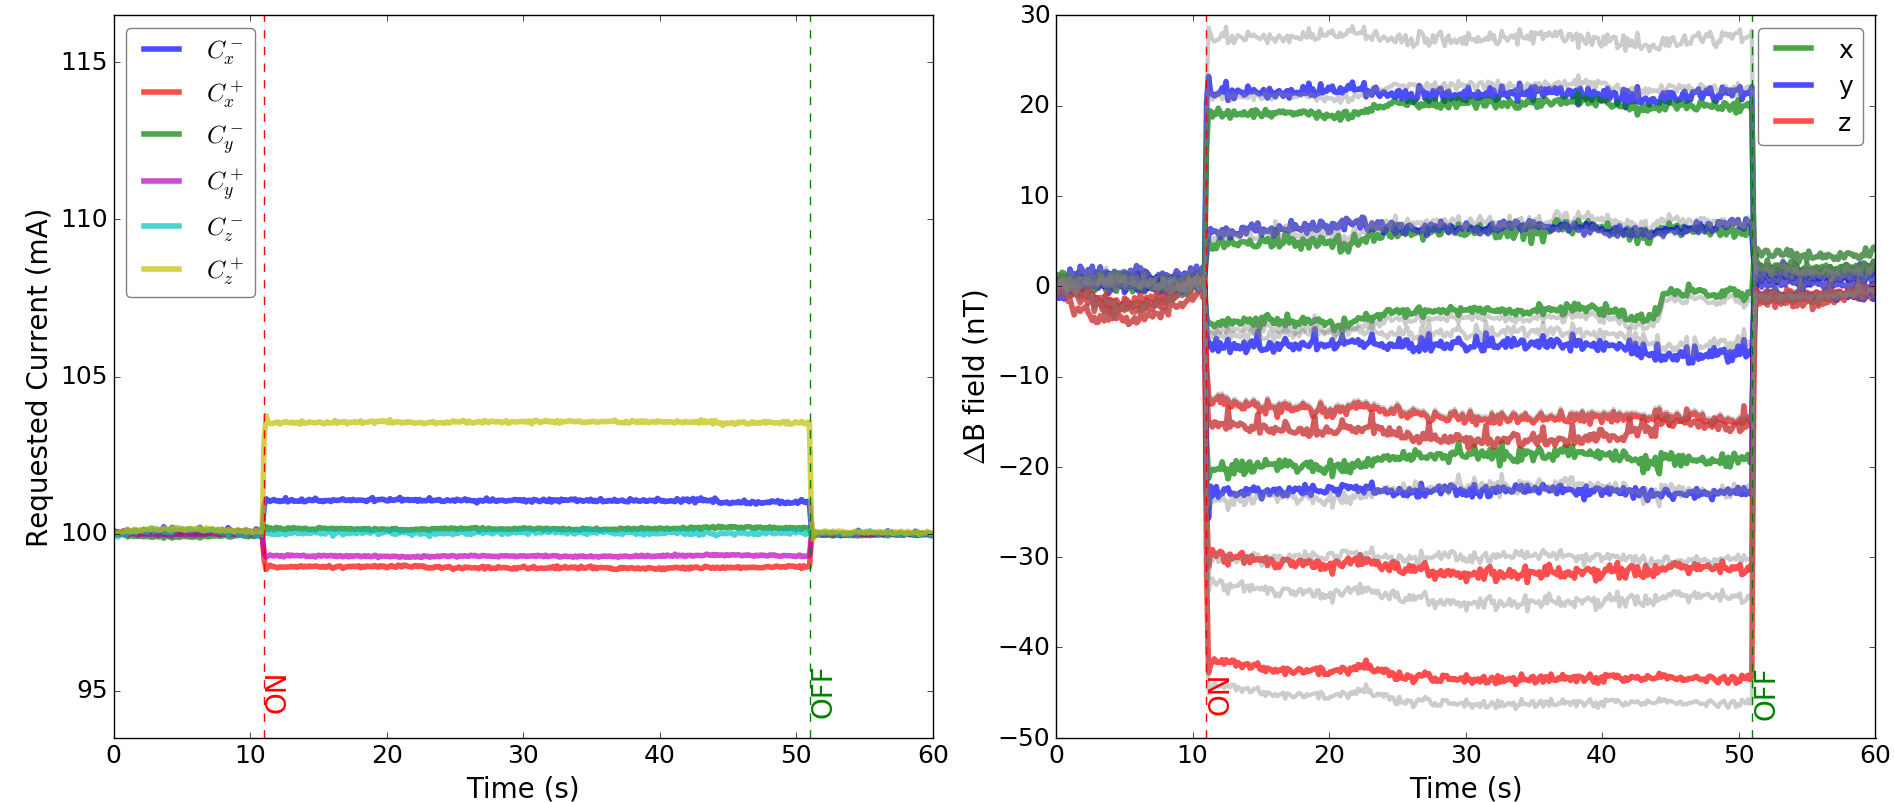
\includegraphics[width=\linewidth, height= 6.5 cm]{Images/p25}
%         \caption{at $k_c^p$=0.25}
%         \label{fig:p25m}
%     \end{subfigure}%
%     \begin{subfigure}{.5\linewidth}
%         \centering
%         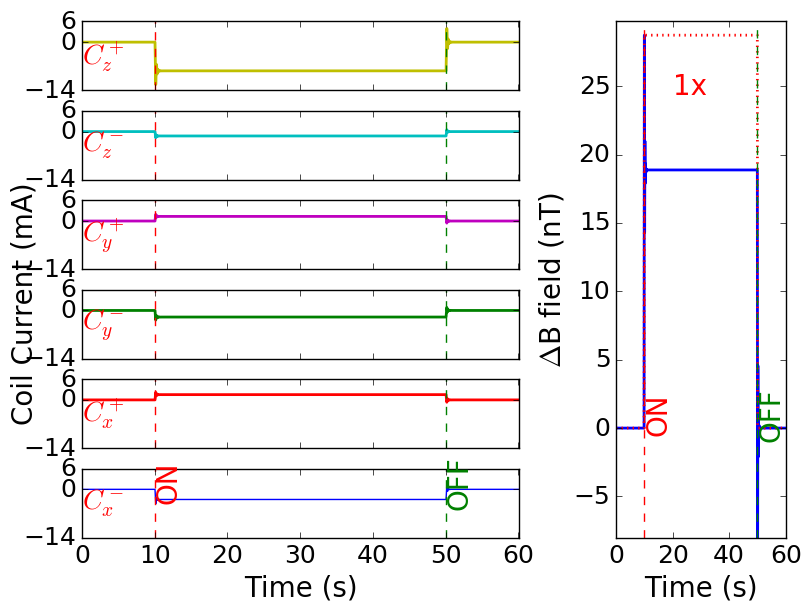
\includegraphics[width=\linewidth, height= 6.5 cm]{Images/p50}
%         \caption{at $k_c^p$=0.50}
%         \label{fig:p50m}
%     \end{subfigure}\\[1ex]
%     \begin{subfigure}{.5\linewidth}
%         \centering
%         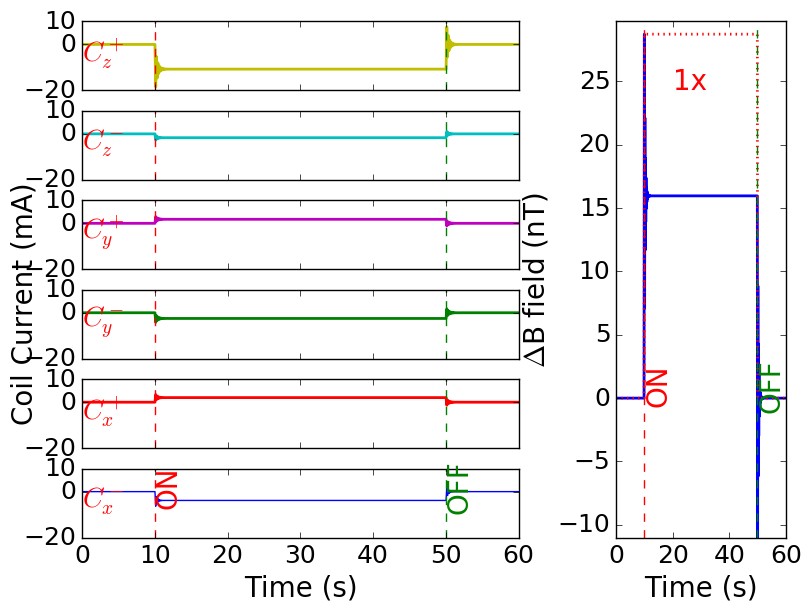
\includegraphics[width=\linewidth, height= 6.5 cm]{Images/p75}
%         \caption{at $k_c^p$=0.75}
%         \label{fig:p75m}
%     \end{subfigure}%
%         \begin{subfigure}{.5\linewidth}
%         \centering
%         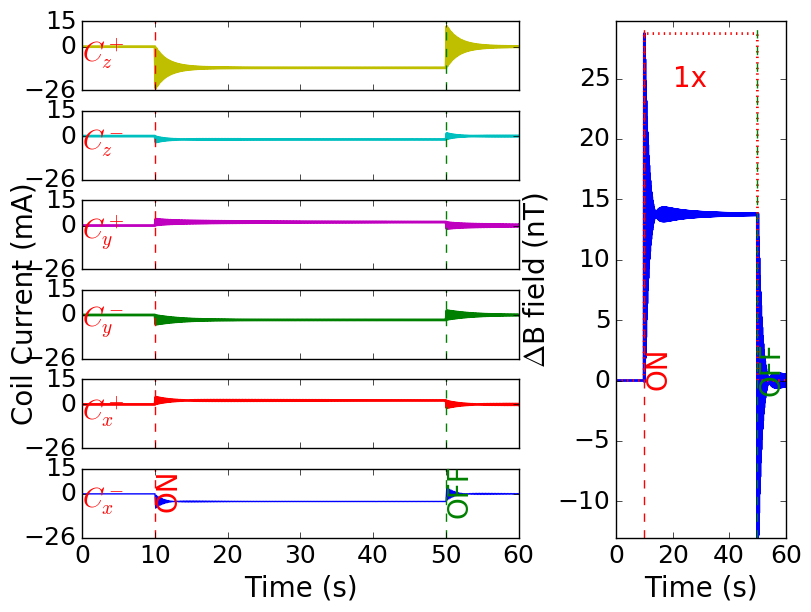
\includegraphics[width=\linewidth, height= 6.5 cm]{Images/p100}
%         \caption{at $k_c^p$=1.0}
%         \label{fig:p100m}
%     \end{subfigure}

%     \caption[short]{Currents (left vertical axis) in all six coil sides ($C_x^\pm$, $C_y^\pm$ and $C_z^\pm$) with drift $\Delta B$ (right vertical axis) at sensor position '1x' for different values of $k_c^p$ with $k_c^i$ in Eq.~(\ref{eq:I}) being zero. Blue color curve denotes the actual drift in signal at position '1x' found by Eq.~(\ref{eq:del_B}) while the red curve denotes the drift that would have been without the compensation. Vertical dashed lines indicate the time of the perturbation coil being turned on and off. For position of coils and sensors see Fig.~\ref{fig:coil}. }
%     \label{fig:p_pi_m}
% \end{figure}

% The effect of changing $k_c^p$ has been shown in Fig.~\ref{fig:p_pi_m} where the currents (left) that are being sent to the coils ($C_x^\pm$, $C_y^\pm$ and $C_z^\pm$) for drift $\Delta B$ found by Eq.~(\ref{eq:del_B}) in sensor position '1x'.  It is seen that $\Delta B$=23 nT, 18.5 nT and 16.5 nT for $k_c^p$ = 0.25, 0.5 and 0.75 respectively (see Fig.~\ref{fig:p_pi_m}\textcolor{blue}{(a)}, Fig.~\ref{fig:p_pi_m}\textcolor{blue}{(b)}, Fig.~\ref{fig:p_pi_m}\textcolor{blue}{(c)}). That is, with the increase of $k_c^p$, $\Delta B$ magnetic field decreases. But, it has a limit after which with the increase of $k_c^p$, the systems becomes unstable and starts oscillating which can be seen from Fig.~\ref{fig:p_pi_m}\textcolor{blue}{(d)}) where the currents (left) are oscillating and the drift itself also at $\Delta B$=14.5 nT (right). So, the error is reduced maximum by (29.5-14.5)/29.5 * 100$\%\approx$51$\%$ from the initial drift of $\Delta B$=29.5 nT denoted by the red curve at position '1x'. 

% 
% The above results confirm that matrix condition number has minimal effect on P term by comparing the effect shown in Section~\ref{sec:pi_behave}. Next, we will discuss about the effect on only I term.

% \subsubsection{Condition Number Effect on Changing only I term}
% Here, the effect matrix condition number effect on changing integral reset term (I) or $k_c^i$ of Eq.~(\ref{eq:I}) will be discussed.

% The error (the difference between setpoint and actual measurement) is accumulated for the length of measurements and I term is multiplying that accumulated error  with a constant gain as discussed in Section~\ref{sec:pi_behave}.




% As like the effect on P, the effect of changing $k_c^i$ has been shown in Fig.~\ref{fig:i_pi_m} where the currents (left) that are being sent to the coils ($C_x^\pm$, $C_y^\pm$ and $C_z^\pm$) for drift $\Delta B$ found by Eq.~(\ref{eq:del_B}) in sensor position '1x' for $k_c^i$=0.25, 0.5, 0.75 and 1.0.  It is seen from Fig.~\ref{fig:i_pi_m}\textcolor{blue}{(a)}, Fig.~\ref{fig:i_pi_m}\textcolor{blue}{(b)}, Fig.~\ref{fig:i_pi_m}\textcolor{blue}{(c)} and Fig.~\ref{fig:i_pi_m}\textcolor{blue}{(d)}). which are correspond to $k_c^i$ = 0.25, 0.75, 1.0 and 1.25 respectively that the error level (right) is $\sim$3.5 nT in every case, the coil currents(left) never settle in any of them which is not he case for low matrix condition number as seen from Fig.~\ref{fig:i_pi}\textcolor{blue}{(a)}, Fig.~\ref{fig:i_pi}\textcolor{blue}{(b)}, Fig.~\ref{fig:i_pi}\textcolor{blue}{(c)} and Fig.~\ref{fig:i_pi}\textcolor{blue}{(d)}) where the condition number is 33 compared to 129 here.

% \begin{figure}[!htb]
%     \begin{subfigure}{.5\linewidth}
%         \centering
%         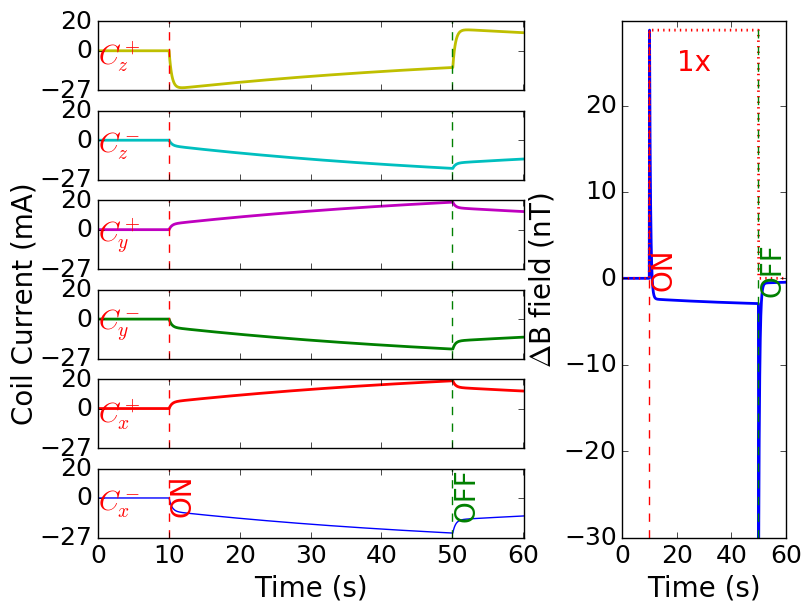
\includegraphics[width=\linewidth, height= 6.5 cm]{Images/i25}
%         \caption{at $k_c^i$=0.25}
%         \label{fig:i25m}
%     \end{subfigure}%
%     \begin{subfigure}{.5\linewidth}
%         \centering
%         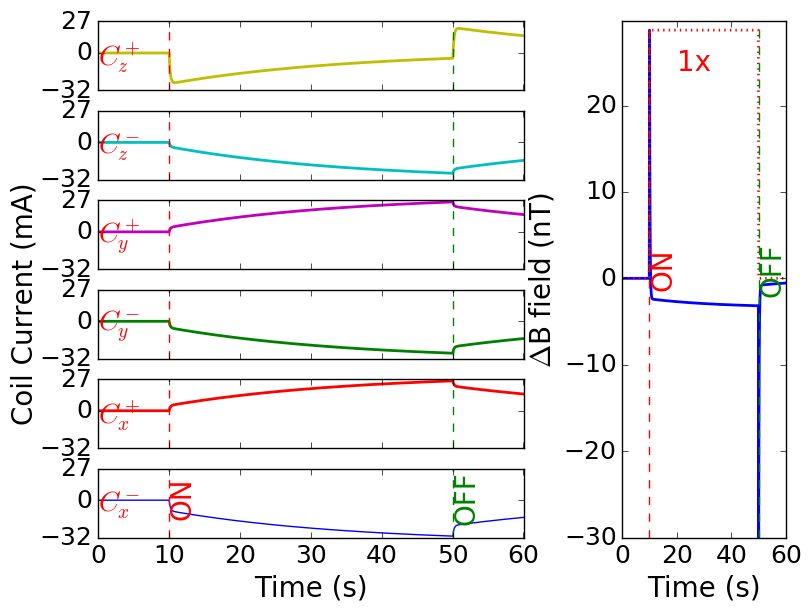
\includegraphics[width=\linewidth, height= 6.5 cm]{Images/i50}
%         \caption{at $k_c^i$=0.5}
%         \label{fig:i50m}
%     \end{subfigure}\\[1ex]
%     \begin{subfigure}{.5\linewidth}
%         \centering
%         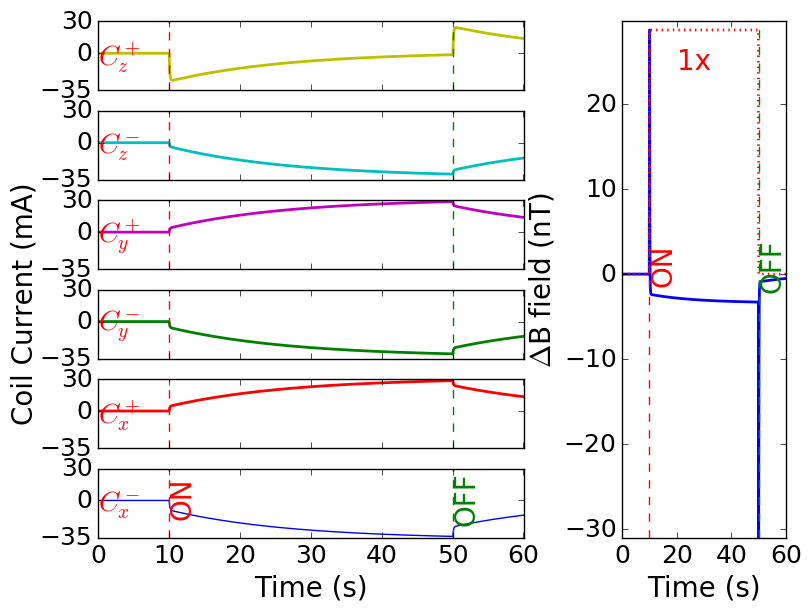
\includegraphics[width=\linewidth, height= 6.5 cm]{Images/i75}
%         \caption{at $k_c^i$=0.75}
%         \label{fig:i75m}
%     \end{subfigure}%
%         \begin{subfigure}{.5\linewidth}
%         \centering
%         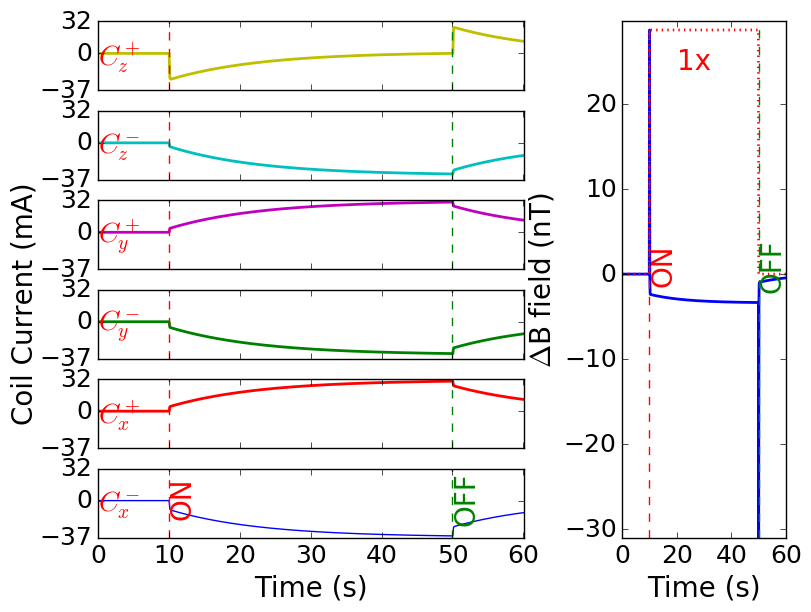
\includegraphics[width=\linewidth, height= 6.5 cm]{Images/i100}
%         \caption{at $k_c^i$=1.0}
%         \label{fig:i100m}
%     \end{subfigure}

%     \caption[short]{Currents (left vertical axis) in all six coil sides ($C_x^\pm$, $C_y^\pm$ and $C_z^\pm$) with drift $\Delta B$ (right vertical axis) at sensor position '1x' for different values of $k_c^i$ with $k_c^p$ ( see Eq.~(\ref{eq:I}) ) being zero. Blue color curve denotes the actual drift in signal at position '1x' found by Eq.~(\ref{eq:del_B}) while the red curve denotes the drift that would have been without the compensation. Vertical dashed lines indicate the time of the perturbation coil being turned on and off. For position of coils and sensors see Fig.~\ref{fig:coil}.}
%     \label{fig:i_pi_m}
% \end{figure}



% % \fig{Images/i_pi_zoom}{width = \textwidth,height =10cm}{Zoomed in version of the drift $\Delta B$ shown in right side of Fig.~\ref{fig:i_pi}\textcolor{blue}{(a)}, Fig.~\ref{fig:i_pi}\textcolor{blue}{(b)}, Fig.~\ref{fig:i_pi}\textcolor{blue}{(c)} and Fig.~\ref{fig:i_pi}\textcolor{blue}{(d)} respectively at sensor position '1x' for different values of $k_c^i$ with $k_c^p$ ( see Eq.~(\ref{eq:I}) ) being zero. The red vertical dashed line indicates the time of the perturbation coil being turned 'ON'. For position of coils and sensors see Fig.~\ref{fig:coil}.\label{fig:i_pi_zoom}}


% 
% The above results confirm the currents in the coils never settles in if there is a ill-conditioned matrix present.. Next the condition number effect on both both of them after tuning (see Section~\ref{sec:tune}) will be discussed and may be the currents settle there!!


% \subsection{r vs. Condition No.}\label{sec:cond}
% Instead of going through all the steps that are discussed in Section~\ref{sec:inv}, the concept of condition number of a matrix can be used. The condition number of $\bm{M}$ can be determined from the diagonal matrix $\bm{\Sigma}$ as given in eq.\ref{eq:m} by -
%  \begin{equation}
%      cond(\bm{M})=\frac{max(\sigma_d)}{min(\sigma_d)}
%  \end{equation}
 

% \subsubsection{Condition Number Effect of changing PI term combined}
% Finally, the Section~\ref{sec:pi_behave_m} will be ended here with the discussion of the condition number effect on changing P and I term at a time which will complete the Eq.~(\ref{eq:I}).

% Here, first the P and I term have been tuned following the discussion on Section~\ref{sec:tune} which has generated $k_c^p$=0.43 and $k_c^i$=0.52 . The results by applying $k_c^p$ and $k_c^i$ as those tuned values are shown in Fig.~\ref{fig:tuned_vs_i}\textcolor{blue}{(a)}. For simplicity instead of showing all the drift $\Delta B$ for all the fluxgate sensors for the positions given in the horizonatal axis of Fig.~\ref{fig:m}, only '1x' is shown on the right of the figure. And same as earlier the currents  that are being sent to the coils ($C_x^\pm$, $C_y^\pm$ and $C_z^\pm$) shown on the left of the same figure. But, we couldn't determine the effect of having both of them at a time. So, keeping $k_c^i$ as 0.52 and excluding P term i.e. $k_c^p$=0.0 we run the same measurement again and the results are shwon in Fig.~\ref{fig:tuned_vs_i_m}\textcolor{blue}{(b)}. The results of Fig.~\ref{fig:tuned_vs_i_m}\textcolor{blue}{(a)} are similar to that of Fig.~\ref{fig:tuned_vs_i_m}\textcolor{blue}{(b)} which is also true for low condition number as discussed in Section~\ref{sec:pi_behave}. 

% \doublefig{Images/p43i52}{width =\textwidth,height =8cm}{at $k_c^p$=0.43 and $k_c^i$=0.52. \label{fig:pi_tuned_m}}{Images/i52}{width = \textwidth,height =8cm}{at $k_c^p$=0.0 and $k_c^i$=0.52..\label{fig:i52m}}{{Currents (left vertical axis) in all six coil sides ($C_x^\pm$, $C_y^\pm$ and $C_z^\pm$) with drift $\Delta B$ (right vertical axis) at sensor position '1x' for combine different values of $k_c^i$ and $k_c^p$ ( see Eq.~(\ref{eq:I}) ). Blue color curve denotes the actual drift in signal at position '1x' found by Eq.~(\ref{eq:del_B}), while the red curve denotes the drift that would have been without the compensation. Vertical dashed lines indicate the time of the perturbation coil being turned on and off. For position of coils and fluxgate sensor see Fig.~\ref{fig:coil}.} \label{fig:tuned_vs_i_m}}{short}

% 
% The above results rather confirm that matrix condition number does not bring any change while using P and  term at a time. But it has got huge impact on I term for which the coil current never settles in case of ill conditioned matrix. Next we will try to improve the current settling problem by changing the regularization parameter.

\subsection{Effect of $r$ on PI Tuning}\label{sec:r_pi}


% \begin{itemize}
% \item We noticed that if we kept P \& I fixed, and changed only $r$, then we'd also get worse current drifting.  But paradoxically, the field would respond quite fast.
% \item It is natural that r should affect PI, because the error function involves $\bm{M^{-1}}$ and therefore $r$.  See e.g.~Eq.~(4.10) for r and (4.3) and (4.4) for how Minv enters the PI algorithm.  If $r$ is big then Minv gets small.  So it would be reasonable to expect that if r increases then we need to crank up both kp and ki accordingly see eq. 4.4.
% \item Consider showing a study where you change P\& I to try to compensate?
% \item We tried this but it didn't work.  Data?  Or simulation?
% \item Lower r seems better Fig.~5.13(a), but what I remember is that when we did that it made the B-noise worse.  Seems like an overcorrected system.  Setting P\& I lower to try to compensate the overcorrection I think made the system slower again (?)
% \item Basic conclusion:  If r or cond is bad (too big) then no amount of PI tuning will help speed up the current drifting.  If r set falsely low, it also doesn't help because it induces HF noise and setting PI large again induces slow response.
% \end{itemize}

The discussion on Section~\ref{sec:pi_behave} suggests that the
$k_c^i$ term in the PI feedback algorithm is necessary for fast system
response, and to reduce proportional droop and hence the error
signals.  But, in including this term, I found that it also creates
problems in terms of the coil currents which take long periods of time
to settle (several tens of seconds).  I called this problem the
current drifting problem.  Adjusting the PI feedback parameters
changed the problem somewhat but ultimately did not reduce the current
drifting time.  Here, I focus on the effect of $r$ on this problem,
treating it on a more equal footing with the PI parameters.


\fig{Images/rp_i}{width=\textwidth,height=8cm}{The $C_z^+$ coil current (left) and magnetic field change $\Delta B$ for sensor 8x (right) with $k_c^p=0.6$, $r=3.04$ and different values of $k_c^i$. In each case, resolution index 1 with 50 software averages per cycle were used. Vertical dashed lines indicate the perturbation coil state.\label{fig:rp_i}}{Single magnetic field compensation results for fixed $k_c^p$ and $r$ and different values of $k_c^i$.}

Fig.~\ref{fig:rp_i} shows an example of the impact of changing $k_c^i$
when $k_c^p$ is held fixed and the regularization parameter $r$ is set
to its best value.  Only the current in one coil and the field
measured in one fluxgate axis are shown so that the impact of changing
$k_c^i$ can be observed.

It is seen that there is no current drifting problem if $k_c^i=0.0$ is
used, but that the field error is consequently larger.  If $k_c^i=0.8$
is used, the field is corrected in a few seconds to a smaller error,
but the current drifts for considerably longer, about 10-20 seconds.
This is similar to the observations described in
Section~\ref{sec:pi_behave}.  We have also seen the effect in
Section~\ref{sec:pi_behave} that increasing $k_c^i$ after a point
makes the current unstable resulting in overshoot.

For these studies, I focused on the $C_z^+$ coil and the 8x sensor
because they are located closer to the pertubation coil and hence see
most of the effect.

\fig{Images/pi_r}{width = \textwidth,height=8 cm}{The $C_z^+$ coil current (left) and magnetic field change $\Delta B$ (right) for sensor 8x with $k_c^p=0.6$, $k_c^i=0.37$ and different values of $r$. In each case, resolution index 1 with 50 software averages per cycle were used. Vertical dashed lines indicate the perturbation coil state.\label{fig:pi_r}}{Single magnetic field compensation results for fixed $k_c^p$ and $k_c^i$ and different values of $r$.}


I then tried changing $r$ while keeping $k_c^i$ and $k_c^p$ terms
fixed.  Fig.~\ref{fig:pi_r} shows the active compensation for same
fluxgate positions and same settings as in Fig.~\ref{fig:rp_i}, with
$k_c^i=0.37$, and this time for different values of $r$. The
observation is that for decreasing $r$, the current drifting problem
disappears, but the feedback system introduces high frequency
noise.

It is natural that $r$ should affect the PI control, because the error
function involves $\bm{M^{-1}}$ and therefore $r$ (see
{\it e.g.}~Eqs.~(\ref{eq:del_I}), (\ref{eq:I}), and (\ref{eq:minvR})).  If
$r$ is larger then $\bm{M^{-1}}$ generally gets small.  So, it would be
reasonable to expect that if $r$ increases then we need to increase
both $k_c^p$ and $k_c^i$ accordingly (see Eq.~(\ref{eq:I})).

\fig{Images/p60i36r24}{width = \textwidth,height=7cm}{Currents (left) in all six coils ($C_x^\pm$, $C_y^\pm$ and $C_z^\pm$) and field change $\Delta B$ (right). The fluxgate positions are 1, 3, 6 and 8.  The feedback and regularization parameters are $k_c^p=0.6$, $k_c^i=0.37$, and $r=2.4$.  The current supplied to the perturbation coil was 10  mA when switch on. Resolution index 1 with 50 averages per cycle were used.\label{fig:pi_tuned_r24}}{Coil currents with field change $\Delta B$ for $k_c^p=0.60$, $k_c^i=0.37$ and $r=2.4$}

The best that can be done to fix the current drifting problem is then
that $r$, $k_c^p$, and $k_c^i$ be adjusted to reduce the current
drifting problem without too much impact on high-frequency noise.  An
example of an attempt to make this trade-off is shown in in
Fig.~\ref{fig:pi_tuned_r24}.  Other than changing $r$ to 2.4, this
Figure uses the same settings as
Fig.~\ref{fig:pi_i_mCond30}\textcolor{blue}{(a)}.  Indeed reducing $r$
has increased the speed with which the currents settle, but an
increase in high-frequency noise on the currents is apparent.
However, this increase in current noise does not increase
the noise on the field measurements noticeably, which is similar in both cases.
In Fig.~\ref{fig:i100_r24}, I have retained this value of $r=2.4$ and
adjusted the PI parameters to attempt to further improve the response
time on the currents.

\fig{Images/p0i100r24}{width = \textwidth,height=7cm}{Currents (left) in all six coils ($C_x^\pm$, $C_y^\pm$ and $C_z^\pm$) and field change $\Delta B$ (right). The fluxgate positions are 1, 3, 6 and 8.  The feedback and regularization parameters are $k_c^p=0.0$, $k_c^i=1.0$, and $r=2.4$.  The current supplied to the perturbation coil was 10  mA when switch on. Resolution index 1 with 50 averages per cycle were used.\label{fig:i100_r24}}{Coil currents with field change $\Delta B$ for $k_c^p=0.0$, $k_c^i=1.0$ and $r=2.4$}

Eventually, I determined that neither of these solutions is truly
optimal.  I now characterize them as being generally
ill-conditioned.  The final solution is discussed further in
Section~\ref{sec:coil_config}.

The above results show that if $r$ (or the condition number) is bad
(too big) then no amount of PI tuning will help speed up the current
drifting.  If $r$ set falsely low, it has the undesirable impact of
inducing high frequency current noise, similar to increasing the PI
parameters, which is expected. While this might be acceptable in some
situations, such as if the field noise is already rather large, it is
not the best general solution.
 



% \begin{itemize}
%     \item message from Fig.~\ref{fig:exp_sim}??
% \end{itemize}

% The experimental setup is same as discussed in Section~\ref{sec:pi_behave_m}. But in this case we have chosen $k_c^p$=0 and $k_c^i$=0.52. Among those $k_c^i$=0.52 has been found due to PI tuning (see Section~\ref{sec:tune}) and instead of choosing  $k_c^p$=0.43 we have made this zero as from the earlier discussion we saw that it barely has any effect while we use the I term. So, these values of $k_c^p$ and $k_c^i$ will be applied on Eq.~\ref{eq:I} to find the currents to be sent to the coils ($C_x^\pm$, $C_y^\pm$ and $C_z^\pm$) for drift $\Delta B$ found by Eq.~(\ref{eq:del_B}) in the sensor positions given in the horizontal axis of Fig.~\ref{fig:m}. So, keeping those fixed, we will try to change the value of $r$ which will modify the Eq.~(\ref{eq:minvR}) for each change of $r$ value.

% The effect of changing $r$ with $k_c^p$=0 and $k_c^i$=0.52 has been shown in Fig.~\ref{fig:r_pi} where the currents (left) that are being sent to the coils ($C_x^\pm$, $C_y^\pm$ and $C_z^\pm$) for drift $\Delta B$ found by Eq.~(\ref{eq:del_B}) in sensor position '1x'.  It is seen from Fig.~\ref{fig:r_pi}\textcolor{blue}{(a)}, Fig.~\ref{fig:r_pi}\textcolor{blue}{(b)}, Fig.~\ref{fig:r_pi}\textcolor{blue}{(c)} and Fig.~\ref{fig:r_pi}\textcolor{blue}{(d)} which are correspond to $r$ = 2.0, 2.4, 2.8 and 3.2 respectively that the changing $r$ has significant effect on the coil current graph and barely any effect on the system response time for reducing the drift in the signal. That is at $r$=2.0, the coil current graph has the fastest settling time where the current settles within 3 s after the perturbation has been applied. At $r$=2.4, it takes 10s for the coil currents to settle in. But at $r$=2.8, it seems like the coil current never settles in which is again improved at $r$=3.2. Note that the here seriously ill conditioned matrix with condtion number 129 has been used and optimized $r$ found by the simulation model is $\sim$2.9 which tells us that the coil settling of the current graph seems to have issue with the that optimized 'r for ill-conditioned matrix. So, instead of taking the optimized $r$ that has been found by the simulation model we may have to choose the lower value of $r$. 

% \fig{Images/exp_sim}{width = \textwidth,height=12cm}{Currents (left vertical axis) in all six coil sides ($C_x^\pm$, $C_y^\pm$ and $C_z^\pm$) with drift $\Delta B$ (right vertical axis) at 12 sensor positions with fluxgate positions 1, 3, 6 and 8 for $k_c^p$=0.0 and $k_c^i$=1.0 (see Eq.~(\ref{eq:I})). For position of coils and fluxgates see Fig.~\ref{fig:coil}. All grey color curves in $\Delta B$ graph denote the drift in signal that would have been without the compensation while all other color curves denote the actual drift in signal at all 12 sensor positions found by Eq.~(\ref{eq:del_B}). Vertical dashed lines indicate the time of the perturbation coil being turned on and off. The current supplied on perturbation coil was 10  mA. The resolution index 1 (see Table~\ref{table:t7freq}) with 50 no of averages per measurement and $r$=3.1 were used. The loop sampling frequency was found to be $\sim$6.5 Hz.\label{fig:exp_sim}}{Coil currents with drift $\Delta B$ for $k_c^p$=0.0, $k_c^i$=1.0 and $r$=3.1}







% % \fig{Images/cp0i100r24}{width = \textwidth}{short.\label{fig:m2}}{Short}
% \begin{itemize}
%     \item message from Fig.~\ref{fig:pi_tuned_r24}??
%     \item current drifting in Fig.~\ref{fig:tuned_vs_i} is hugely reduced in Fig.~\ref{fig:pi_tuned_r24}. 
% \end{itemize}


% \begin{figure}[!htb]
%     \begin{subfigure}{.5\linewidth}
%         \centering
%         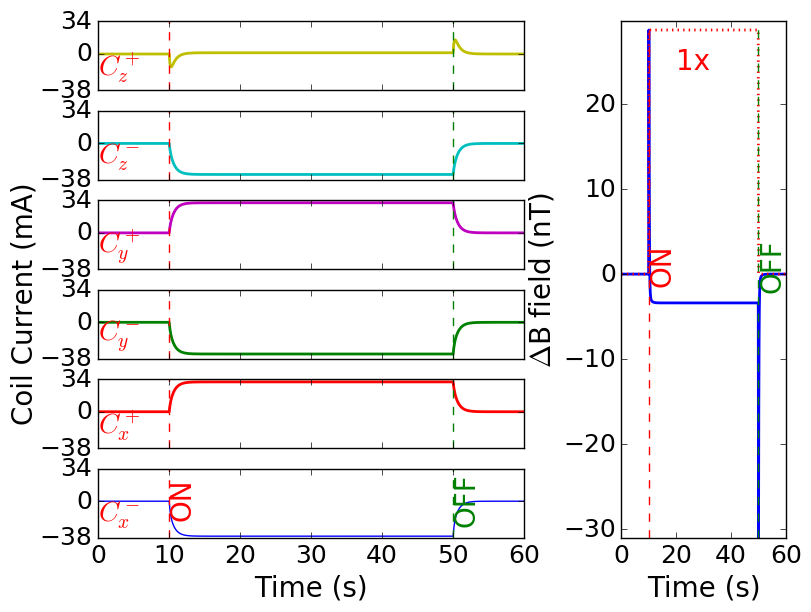
\includegraphics[width=\linewidth, height= 6.5 cm]{Images/r20}
%         \caption{at r=2.0}
%         \label{fig:r20}
%     \end{subfigure}%
%     \begin{subfigure}{.5\linewidth}
%         \centering
%         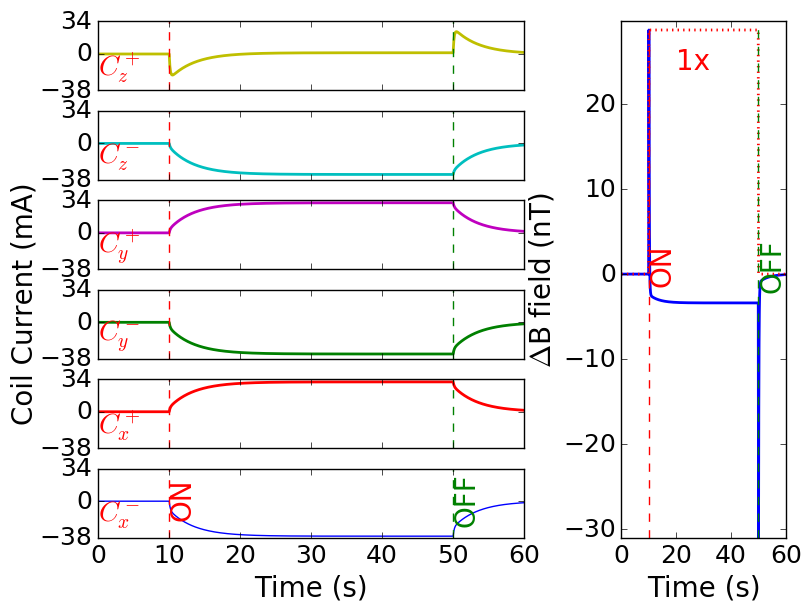
\includegraphics[width=\linewidth, height= 6.5 cm]{Images/r24}
%         \caption{at r=2.4}
%         \label{fig:r24}
%     \end{subfigure}\\[1ex]
%     \begin{subfigure}{.5\linewidth}
%         \centering
%         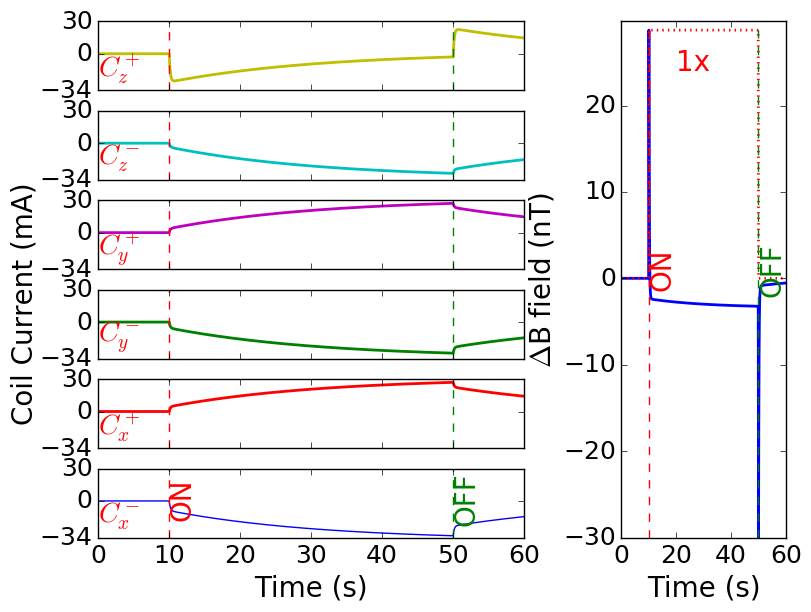
\includegraphics[width=\linewidth, height= 6.5 cm]{Images/r28}
%         \caption{at r=2.8}
%         \label{fig:r28}
%     \end{subfigure}%
%         \begin{subfigure}{.5\linewidth}
%         \centering
%         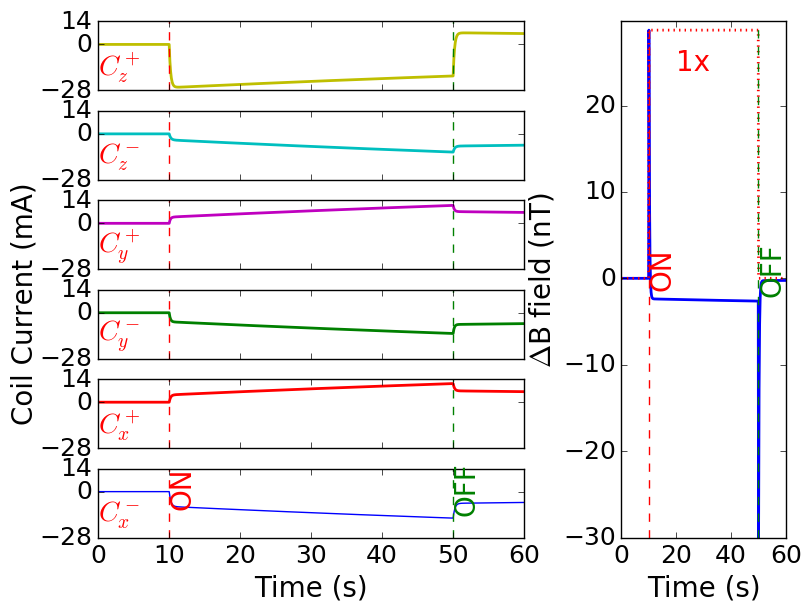
\includegraphics[width=\linewidth, height= 6.5 cm]{Images/r32}
%         \caption{at r=3.2}
%         \label{fig:r32}
%     \end{subfigure}


%     \caption[short]{Currents (left vertical axis) in all six coil sides ($C_x^\pm$, $C_y^\pm$ and $C_z^\pm$) with drift $\Delta B$ (right vertical axis) at sensor position '1x' for combine different values of $k_c^i$ and $k_c^p$ ( see Eq.~(\ref{eq:I}) ). Blue color curve denotes the actual drift in signal at position '1x' found by Eq.~(\ref{eq:del_B}), while the red curve denotes the drift that would have been without the compensation. Vertical dashed lines indicate the time of the perturbation coil being turned on and off. For position of coils and fluxgate sensor see Fig.~\ref{fig:coil}.}
%     \label{fig:r_pi}
% \end{figure}


% Now the question arises about what if $r$ value is chosen more than the optimized $r$. For answering that question, we have also studied the effect for more values of $r$ with same setup which are shown in Fig.~\ref{fig:r_pi_more}. It is seen from Fig.~\ref{fig:r_pi_more}\textcolor{blue}{(a)}, Fig.~\ref{fig:r_pi_more}\textcolor{blue}{(b)}, Fig.~\ref{fig:r_pi_more}\textcolor{blue}{(c)} and Fig.~\ref{fig:r_pi_more}\textcolor{blue}{(d)} which are correspond to $r$ = 3.5, 3.6, 3.7 and 3.9 respectively that the coil current graph seems to be settle in for larger value of $r$ before it starts showing less responsive for example at $r$=3.9.   

% \begin{figure}[!htb]
%     \begin{subfigure}{.5\linewidth}
%         \centering
%         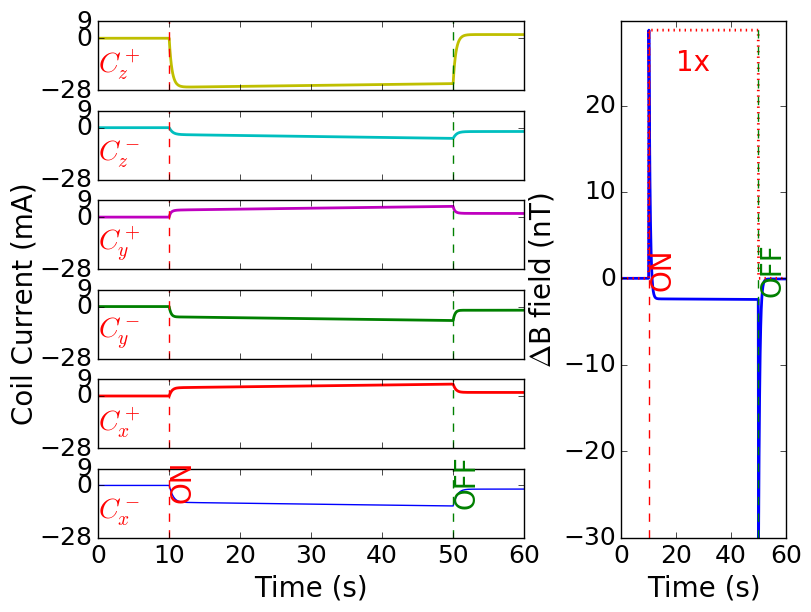
\includegraphics[width=\linewidth, height= 6.5 cm]{Images/r35}
%         \caption{at r=3.5}
%         \label{fig:r35}
%     \end{subfigure}%
%     \begin{subfigure}{.5\linewidth}
%         \centering
%         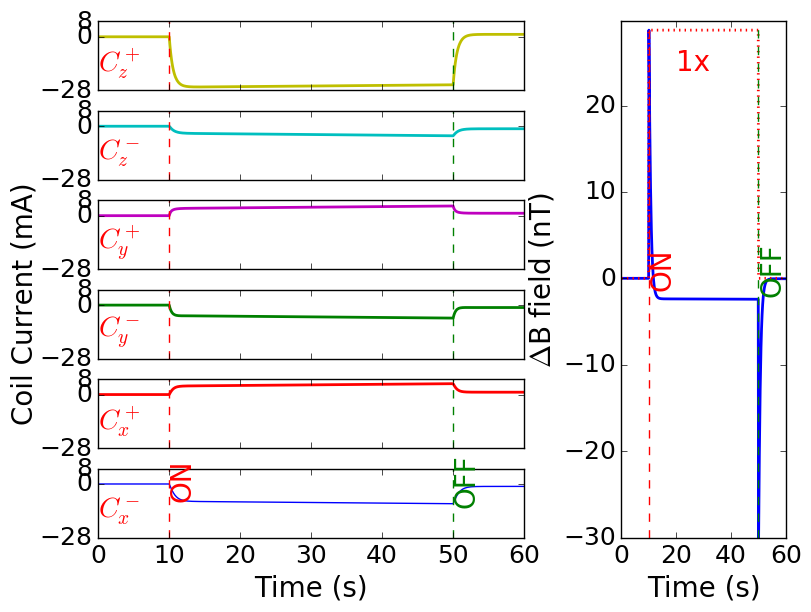
\includegraphics[width=\linewidth, height= 6.5 cm]{Images/r36}
%         \caption{at r=3.6}
%         \label{fig:r36}
%     \end{subfigure}\\[1ex]
%     \begin{subfigure}{.5\linewidth}
%         \centering
%         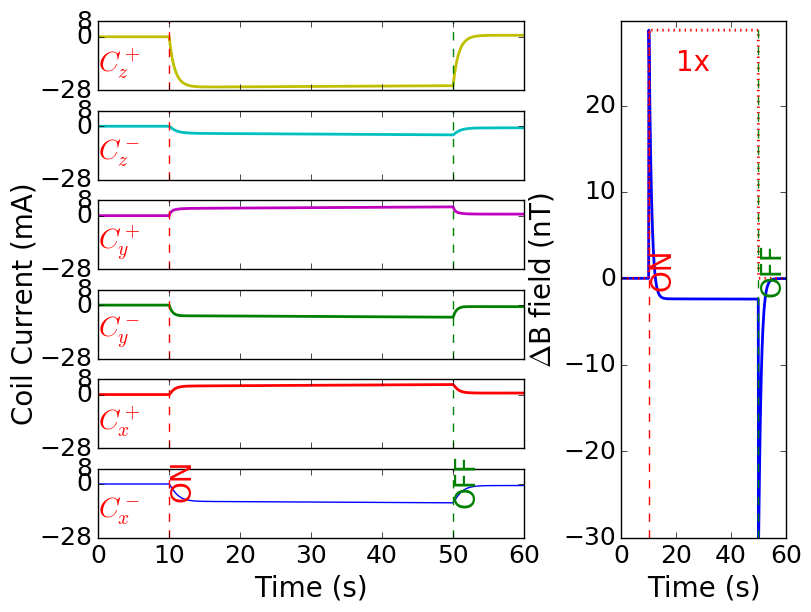
\includegraphics[width=\linewidth, height= 6.5 cm]{Images/r37}
%         \caption{at r=3.7}
%         \label{fig:r37}
%     \end{subfigure}%
%         \begin{subfigure}{.5\linewidth}
%         \centering
%         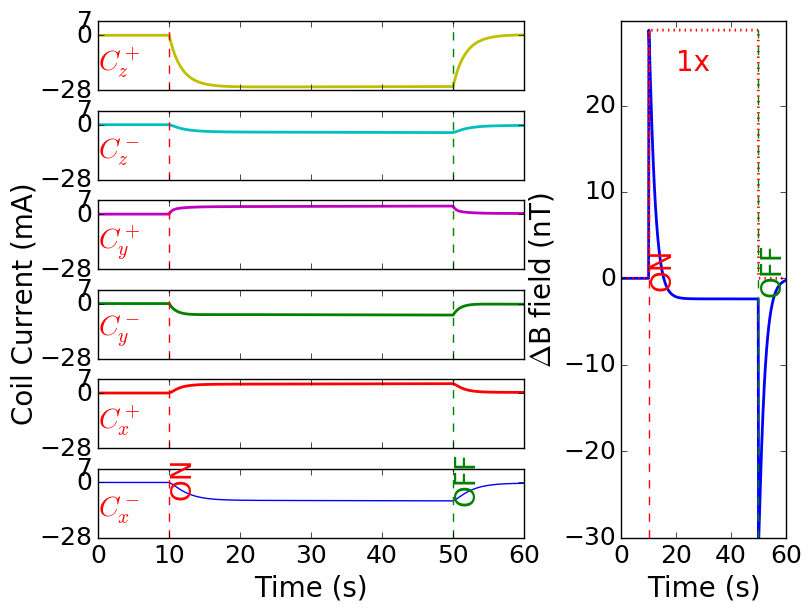
\includegraphics[width=\linewidth, height= 6.5 cm]{Images/r39}
%         \caption{at r=3.9}
%         \label{fig:r39}
%     \end{subfigure}


%     \caption[short]{Currents (left vertical axis) in all six coil sides ($C_x^\pm$, $C_y^\pm$ and $C_z^\pm$) with drift $\Delta B$ (right vertical axis) at sensor position '1x' for combine different values of $k_c^i$ and $k_c^p$ ( see Eq.~(\ref{eq:I}) ). Blue color curve denotes the actual drift in signal at position '1x' found by Eq.~(\ref{eq:del_B}), while the red curve denotes the drift that would have been without the compensation. Vertical dashed lines indicate the time of the perturbation coil being turned on and off. For position of coils and fluxgate sensor see Fig.~\ref{fig:coil}.}
%     \label{fig:r_pi_more}
% \end{figure}



% The above results confirm that for a matrix with large condition number, the value of $r$ has to be tuned alongside the PI tuning. Next we will talk about a new method to find $r$.

\subsection{Regularization by Matrix Condition Number Method  }\label{sec:cond}

%\begin{itemize}
%\item This previous stuff plus Rawlik made us believe that cond number is important.  It's important to make it small.
%\item We noticed another relationship between condition number and regularization parameter for this system:  the best r determined by MC method gave the smallest cond \#.  Fig. 5.15 shows that when r is varied there is a minimum cond \#.  We tested this for a broad variety of M both theoretical and experimental and found it to be always true that the MC method gave the same best r as if we had just selected the one that gives the smallest cond number.
%\item We suspect this is because Tikhonov regularization minimizes both RMS current as well as field fluctuations.  cite Wikipedia (I mean some Tikhonov thing).  In Wikipedia, it minimizes Gammax2 + Ax2.  L2 reg.
%\item So it's not surprising and could be more useful, not requiring an random number technique to find the best r.
%\item Maybe add example graph somehow comparing to the MC technique?
%\end{itemize}


The condition number of $\bm{M}$ and its regularized pseudoinverse,
and the regularization parameter $r$ were introduced in
Section.~\ref{sec:m} while discussing the inversion of the matrix
$\bm{M}$ . Moreover, in Section~\ref{sec:mont}, the method of
Ref.~\cite{bea} of selecting the best value for $r$ by randomly
generated field perturbations was discussed.  The purpose of this
section is to report that this method of selecting $r$ is equivalent
to minimizing the condition number of the regularized pseudoinverse
$\bm{M^{-1}}$.

%  Recall from Section~\ref{sec:inv}, regularization is needed in the first place while inverse of the matrix $\bm{M}$ because $\bm{M}$ itself is ill-conditioned matrix. That means the $\bm{M}$ has a large condition number which while inverse would produce large currents in some ill-positioned places that will make the system unstable. So, it is required to have a well-conditioned  $\bm{M^{-1}}$ which implies that the condition number of $\bm{M^{-1}}$ should be small and that's what regularization has been doing. So, 
 
%We introduce Eq.~\ref{eq:minvR} with various values of $r$ and each time the condition number of $\bm{M^{-1}}$ is stored. Then the optimized $r$  has been determined by selecting the $r$ for which the condition number of $\bm{M^{-1}}$ is the minimum.

\fig{Images/mc_Mcond2}{width = \textwidth,height =7cm}{(a) Condition number of $\bm{M}^{-1}$ vs.~$r$, and (b) determination of $r$ using random field fluctuations.  For a more complete description of (b) see Fig.~\ref{fig:I-fluc}.\label{fig:cond}}{Comparing $r$ from two different methods.}

The condition number of $\bm{M^{-1}}$ for different values of $r$ is
presented in Fig.~\ref{fig:cond}\textcolor{blue}{(a)} and exhibits a
clear minimum at $r=2.90$ (indicated by the red diamond in the
Figure).  It is seen that for $r=0$, the condition number of
$\bm{M^{-1}}\approx 51$ which is by definition the same as the
condition number of $\bm{M}$ itself.  The minimum value of the
condition number is 3.2 which is a factor of 17 reduction.  Recall
that the ideal value of the condition number is unity.

Fig.~\ref{fig:cond}\textcolor{blue}{(b)} shows the same matrix being
analyzed using the random field fluctuation method of
Section~\ref{sec:mont} and Ref.~\cite{bea}, where current fluctuations
are traded off against field control.  In this study, the ``best''
value $r=2.88$ is determined, which can be compared to $r=2.90$ which
minimizes the condition number of the regularized pseudoinverse.

I tried this same comparison for a variety of different $\bm{M}$ and
always found the same level of agreement in the determination of $r$.
A sample of results was shown in Table~\ref{table:flux-pos}.  I think
that the method of minimizing the condition number is more robust
because it does not involve random number generation and therefore is
free of any additional statistical error.

I suspect the excellent agreement seen between the two methods results
from the definition of Tikhonov
regularization~\cite{tikhonov2013numerical,tikhonov_book,svd,svd3}.

Given a vector of field fluctuations $\Delta\vec{B}$ and a vector of
correction currents $\Delta\vec{I}$, the Moore-Penrose pseudoinverse
$\bm{M}^{-1}$ can be thought of as the matrix which minimizes
$|\Delta\vec{I}-\bm{M}^{-1}\Delta\vec{B}|$, which is analogous to
chi-squared minimization for a system of linear equations.  Tikhonov
regularization is used when this problem becomes ill conditioned, and
introduces another constraint that simultaneously minimized the modulus of the vector
$|\Delta\vec{I}|$ . In a way this is equivalent to the compromise being
made in the selection of the ``best'' $r$ using the random field
fluctuation method.  Current and field fluctuations are being traded
off against one another in order to prevent large current fluctuations
from occurring.




I think, it is therefore not surprising that the two methods give good
agreement. I feel the minimization of condition number is a better
defined solution, not requiring random number generation, and that it
is a superior and robust method to determine $r$.


% \subsubsection{Optimized r  Revisited Based on Current Response Time}\label{sec:r_currentResponse}
% It was found that there is very slow coil current rise time while applying perturbation. To get rid of that problem, first and foremost, the fastest sampling frequency (see section [\ref{sec:filter}, \ref{sec:freq}]) is needed. Then, the next step of the problem can be solved via two ways with individual having own limitations. First way is tuning the value of P and I term of PI loop as explained in Eq.~(\ref{eq:I} and Section~\ref{sec:tune}. But with increasing the value of P, the current start oscillating after certain values as shown by the top and middle current graph on Fig.~\ref{fig:crnt} which is a problem. 

% \fig{Images/crnt}{width = \textwidth}{Coil current in one of the coil side for optimized r=2.8 with P=0 and I=1.0 (top) and with P=0 and I=1.5 (middle) and for best r considering noise with P=0 and I=1.0 (bottom). \label{fig:crnt}}



% The alternative way is to change the value of optimized r (see section [\ref{sec:mont}, \ref{sec:cond}]) which in turns increase noise in the prototype. But with inclusion of some current fluctuations, it was found that the coil current response time was increased heavily  as shown by the bottom current graph in Fig.~\ref{fig:crnt}. Now, the best compromised value of r was chosen by observing the 'rise time vs r' and 'fluctuations vs r' as shown in Fig.~\ref{fig:riseT}.



%  \doublefig{Images/riseT}{width =\textwidth, height= 8 cm}{Rise Time vs r \label{fig:rise}}{Images/fluc}{width = \textwidth, height= 8 cm}{Fluctuations\label{fig:fluc}}{{(a) shows the Rise Time vs r (b) shows the Fluctuations } \label{fig:riseT}}
% % \fig{Images/bt}{width = \textwidth}{Magnetic Field Compensation \label{fig:bt}}






% \section{Fluxgate Placements and Impact of Shields}\label{sec:flux_place}


% \begin{itemize}
% \item We still had no clue so we just started changing things randomly.
% \item We changed fluxgate positions to try to make cond number smaller to see if it had an effect.  Could not change the cond number or the problem significantly.
% \item We were confused if the slow current response might be due to magnetic responses that we slow.  So we tried removing the shields.  No change.
% \item consider a graph where there is current drifting but with no shield.
% \item And then we realized this had nothing to do with it.
% \end{itemize}

% In earlier section we have shown results using 12 fluxgate sensors placed at positions as given in horizontal axis of Fig.~\ref{fig:m} and there exact positions are described by the Fig.~\ref{fig:coil}. We were facing serious problem with coil current not being settle properly although the field seems to be compensated on time. So, we have tried different positions mainly in corners and center of each of the coil faces. Even, we have removed the outermost shields also. In this Section, the results of those studied will be shown and discussed. 

% First the study on the fluxgate placement will be discussed.

% \subsection{Fluxgate Placements}

% We have not got clear idea about the placements of the fluxgates from the previous studies and our coil current also did not settle down the way we thought is should. We have started taking data with 3*4=12 sensors at slowest sampling frequency (see Table~\ref{table:index}) in the corners but the coil currents were not properly settle down. Then we thought maybe increasing sensors will eliminate the problems. So, we bought new fluxgate sensors and build another breakout box (see Section~\ref{sec:sensor}) but still the results were not good in the coil currents. Then we thought may be if we place in the center of each of the faces of the coils the results will be better but unlucky us. Then we decided to remove the outermost shield (see Section~\ref{sec:shield}) to see the effect but still no luck. After that we decided to use the fastest sampling frequency of our ADC for which we have to build the filters. But due to time limitations and cost concern we have only build 12 filters to support 12 fluxgate sensors. Now, due to this the current response time has increased but that was not the solution of the current unsettle problem. Finally, we have realized that in addition to fastest response we have to also consider the matrix condition number and if the condition number is large then we have to lower the value of optimized $r$ (see Section~\ref{sec:new_study_r}). Here, we will talk about the the studies we have done on fluxgate placements.

% \begin{table} [htb!]
%     \centering
%     \begin{tabular} { |c|c|c|c|c|c|} 
%         \hline
%         \makecell{Fluxgates \\Position} & \makecell{$\bm{M}$\\ Condition No.} &\makecell{$\bm{M^{-1}}$\\ Condition No.} & $r$ & $r'$\\
%         \hline\hline
%         1, 3, 6 and 8 & 33.25 & 2.63 & 2.97 & 2.95\\ 
%         \hline
%         2, 4, 5 and 7 & 28.55 & 1.98 & 3.04 & 3.06 \\ 
%         \hline
%         \makecell{Center \\($C_x^\pm$, $C_y^\pm$ and $C_z^\pm$)} & 36.24 & 1.8 & 2.47 & 2.49 \\ 
%         \hline
%         \makecell{Center-6cm \\($C_x^\pm$, $C_y^\pm$ and $C_z^\pm$)} & 98.61 & 3.05 & 2.36 & 2.34 \\ 
%         \hline
%         \makecell{Center+6cm \\($C_x^\pm$, $C_y^\pm$ and $C_z^\pm$)} & 80.74 & 1.49 & \textcolor{red}{2.26} & \textcolor{red}{2.02} \\ 
%         \hline
%         \makecell{1, 2, 3, 4, \\5, 6, 7 and 8} & 28.30 & 1.94 & 3.17 & 3.19 \\ 
%         \hline
%         \makecell{1, 2, 3, 4, \\5, 6, 7, 8 and \\Center ($C_x^\pm$, $C_y^\pm$ and $C_z^\pm$)}  & 21.84 & 1.8 & \textcolor{red}{3.23} & \textcolor{red}{3.37} \\ 
%         \hline

%     \end{tabular}
%     % \vspace{4mm}
%     \caption[Properties of different no of fluxgate sensors for different positions.]{Properties of different no of fluxgate sensors for different positions. For the positions of the fluxgates see Fig.~\ref{fig:coil} }\label{table:flux-pos}
% \end{table}

% Mainly the corner positions and the center of each of the coil faces  have been tested. Also, they have been analyzed by moving slightly in different positions. The results for different no of sensors in different positions are given in Table~\ref{table:flux-pos}. Position of the fluxgates are defined by the numbers while they are in corners and when they are in the center of each of the coil faces they are termed as 'Center ($C_x^\pm$, $C_y^\pm$ and $C_z^\pm$)'. Center-6cm means all the sensors in the center of the coil faces have been brought 6cm towards the origin from the center and center+6cm means they have brught 6cm away outside the center. For, the full picture of the positions see Fig.~\ref{fig:coil}. the It is seen that that matrix condition number is from 22-36 for the fluxgates being placed either in corners or in center. But if they are slightly moved within $\pm$6cm of center then the matrix condition number becomes very large. Only considering the matrix condition number, it seems that having fluxgates in all the corners and the center of each of the coil faces should be the best choice as its giving the lowest condition number which is 22. But that is not the whole story! To quantify more we have taken the help of regenerating Fig.~\ref{fig:Isim} and Fig.~\ref{fig:fluc-sim}. From Fig.~\ref{fig:Isim}, we have recorded the maximum  $\Delta I_c^{\text{simRMS}}$ (mA) for 30 different sets of $B_s^{\text{rand}}$. For maximum compensation we have generated the Fig.\ref{fig:fluc-sim} for same for 30 different sets of $B_s^{\text{rand}}$ from which we have recorded lowest the remaining fluctuation F. For example- for fluxgate positions 1, 3, 6 and 8, the lowest F goes to 0.3. That means the maximum compensation due to the field produced by $\Delta I_c^{\text{sim}}$to counteract $B_s^{\text{rand}}$ is(1-0.3$\times$100$\%$) =70$\%$. For more details see Section~\ref{sec:mont}. It seen that the current goes crazy if the fluxgates are placed in the center of the coil faces and the maximum $\Delta I_c^{\text{simRMS}}$ ranges from 98 to 192 mA. But the maximum $\Delta I_c^{\text{simRMS}}$ is 12 mA when the center fluxgates are used with the corners one. But on that time the maximum compensation due to the field produced by $\Delta I_c^{\text{sim}}$to counteract $B_s^{\text{rand}}$ is only 15$\%$. So, anything with center seems to give crazy results. Then by looking at the all the three parameters e.g. matrix condition number, maximum $\Delta I_c^{\text{simRMS}}$ and maximum compensation for the 3 different sets of corner positions only, it is seen that the results are more balanced and surprisingly the compensation with 4*3-axis sensors are better than 8*3-axis sensors in exchange of more maximum $\Delta I_c^{\text{simRMS}}$.


% 


% % The increase in matrix condition number for the center of the coil sides is noteworthy.  So, a study has been done to see the current response effect while sensors are in the middle of the coil sides as shown in Fig.~\ref{fig:cb_center}. The Fig.~\ref{fig:cb_center_p} represents the current response on all the six coil sides with their effect on the $z$-axis in the origin as shown in the right with only choosing proportional (P) term. But just adding a small fraction of integral resest (I) term makes the current response unstable as shown in Fig.~\ref{fig:cb_center_pi}. So only P controller is suitable if fluxgates are placed in the middle of the coil sides but in the case of corner positions either P only or I only or PI controller option is available. In a summary, the more the sensors the more is the matrix condition number. Corner positions are better in terms of different freedom of controlling.

% % \doublefig{Images/cB_t_center_p}{width =\textwidth, height= 6 cm}{Position=1,2,3,4,6,8\label{fig:cb_center_p}}{Images/cB_t_center_pi}{width = \textwidth, height= 6 cm}{Position=1,2,3,4,6,8\label{fig:cb_center_pi}}{{PI Active Magnetic Field Compensation Results by both Experiment and Simulation.} \label{fig:cb_center}}

% % \doublefig{Images/bt6}{width =\textwidth, height= 7 cm}{Position=1,2,3,4,6,8\label{fig:bt6}}{Images/sf6}{width = \textwidth, height= 7 cm}{Position=1,2,3,4,6,8\label{fig:sf6}}{{PI Active Magnetic Field Compensation Results by both Experiment and Simulation.} \label{fig:btSF6}}

% % \doublefig{Images/bt8}{width =\textwidth, height= 7 cm}{Position=1,2,3,4,5,6,7,8\label{fig:bt8}}{Images/sf8}{width = \textwidth, height= 7 cm}{Position=1,2,3,4,5,6,7,8\label{fig:sf8}}{{PI Active Magnetic Field Compensation Results by both Experiment and Simulation.} \label{fig:btSF8}}
% The above discussion of the Table~\ref{table:flux-pos} shows that current goes crazy if the fluxgates are placed in the center of each of the coil faces and crazier if they are slightly moved inside or outside of the center. The corners position fluxgates shows normal behaviour compare to the center positions and surprisingly less sensors shows better compensation in the corners in exchange more more currents.

% 
% \subsection{Different Shields}

% There are four layers of shields have been used for passive shielding in this prototype (see Section~\ref{sec:shield}). The active compensation effect has been seen using outermost shield and no shields. Both of the configurations produce similar results.

% \begin{itemize}
%      \item message from Fig.~\ref{fig:shield_noShield}??
%  \end{itemize}

% % except for the case of shield, the matrix condition number is less. The Fig.~\ref{fig:btSF8_s} shows the AMC compensation (Fig.~\ref{fig:bt8_s}) and the corresponding allan deviation and shielding factor ( Fig.~\ref{fig:sf8_s}) with outermost layer of shield. The matrix condition number is found to be 19. Similarly, the Fig.~\ref{fig:btSF8} shows the AMC compensation (Fig.~\ref{fig:bt8}) and the corresponding allan deviation and shielding factor ( Fig.~\ref{fig:sf8}) without any shield. The matrix condition number in this case is 132. The one advantage of having shielding is that , the shielding factor for all the sensors remain $geq$1 but in case of no shield, the shielding factor may be very good at certain point but in some point it can go below 1.

% \fig{Images/shield_noShield}{width = \textwidth,height=12cm}{Currents (left vertical axis) in all six coil sides ($C_x^\pm$, $C_y^\pm$ and $C_z^\pm$) with drift $\Delta B$ (right vertical axis) at 12 sensor positions with fluxgate positions 1, 3, 6 and 8 for $k_c^p$=0.0, $k_c^i$=1.0 (see Eq.~(\ref{eq:I})) and $r$=2.8. For position of coils and fluxgates see Fig.~\ref{fig:coil}. All grey color curves in $\Delta B$ graph denote the drift in signal that would have been without the compensation while all other color curves denote the actual drift in signal at all 12 sensor positions found by Eq.~(\ref{eq:del_B}). Vertical dashed lines indicate the time of the perturbation coil being turned on and off. The current supplied on perturbation coil was 25  mA. The resolution index 1 (see Table~\ref{table:t7freq}) with 50 no of averages per measurement used. The loop sampling frequency was found to be $\sim$6.5 Hz.\label{fig:shield_noShield}}{Coil currents with drift $\Delta B$ for $k_c^p$=0.0, $k_c^i$=1.0 and $r$=2.8}

% % \doublefig{Images/bt8_shield}{width =\textwidth, height= 7 cm}{Position=1,2,3,4,6,8\label{fig:bt8_s}}{Images/sf8_shield}{width = \textwidth, height= 7 cm}{Position=1,2,3,4,6,8\label{fig:sf8_s}}{{Shield} \label{fig:btSF8_s}}{short}

% % \doublefig{Images/bt8}{width =\textwidth, height= 7 cm}{Position=1,2,3,4,5,6,7,8\label{fig:bt8}}{Images/sf8}{width = \textwidth, height= 7 cm}{Position=1,2,3,4,5,6,7,8\label{fig:sf8}}{{No SHield} \label{fig:btSF8}}{short}



\section{``New'' feedback algorithm vs.~standard PI control}\label{sec:style_pi}

%\begin{itemize}
%\item We were led astray by M. Rawlik in late 2017 (nEDM2017).  It is also written in his thesis.
%\item The claim is that the PI algorithm is not necessary.  Just use this magic new algorithm and you don't need PI any more.
%\item Describe the algorithm and its difference compared to typical PI (our understanding).  Our implementation included P and I terms also.  The main difference seemed to be that I0 wasn't used but rather In in order to determine In+1.
%\item In our implementation we noticed experimentally that kp=1 in the new system corresponded to ki=1 in the old system.
%\item Eventually we figured out why (derivation).
%\item Main conclusion:  the ``New PID'' is the ``old PID'' but with a very particular choice ki=1 and kp=0.  It is clearly better to allow more freedom in the algorithm than this.  Old PID is therefore more general.  Although indeed ki=1 and kp=0 generally do seem to be close to optimal, we think this is a coincidence rather than physics.  We also note the time delays inserted into Rawlik's algorithm are themselves a form of tuning.
%\item So we use regular PI and treat the parameters as TBD by system tuning.
%\end{itemize}

In Sections~\ref{sec:tune} and \ref{sec:pi_behave}, I discussed the PI
feedback algorithm and my studies of tuning both the PI parameters and
the regularization parameter $r$. The studies were all based on the
work of Ref.~\cite{bea}.

Subsequently, Refs.~\cite{rawlik,rawkliknedm2017,rawlikpriv} made the
claim that there is no need to use the standard PI feedback algorithm.
This led to a number of studies using the ``new'' feedback algorithm,
which indeed seemed to give similar results when compared to the
``old'' feedback algorithm.

Eventually, I determined this is due to the fact that they are
mathematically equivalent under certain conditions which correspond
closely to the typical operating conditions of my active magnetic
compensation apparatus.

The basis of the ``new'' feedback algorithm is presented in
Ref.~\cite{rawlik} as providing an updated version of current
$\vec{I^{n+1}}$ which is based on the current determined by the previous
step $\vec{I^n}$.  The equation to be used to find the next current in the
new algorithm is
\begin{equation}\label{eq:I_raw}
    \vec{I^{n+1}}= \vec{I^n}+\bm{M^{-1}} (\vec{B_{\rm setpoint}}-\vec{B_{\rm
    measure}^n})=\vec{I^n}+\bm{M^{-1}} \Delta \vec{B^n}
\end{equation}
which is taken directly from Eq.~\textcolor{blue}{(28)} in Section~\textcolor{blue}{5.5} of
Ref.~\cite{rawlik}. In this equation, $\Delta \vec{B^n}$ is a vector of
magnetic field values measured in the given feedback step.  The
dimension is equal to the number of fluxgate axes being used for
control (12 in my case).  The quantity $\bm{M^{-1}}$ is the Moore-Penrose
pseudoinverse (a $6\times 12$ non-square matrix, in my case).  The
quantity $\vec{I^n}$ are a vector of currents (dimension 6, in my case).
The index $n$ refers to the values as of the present feedback step.
The index $n+1$ on the left-hand-side of the equation is indicating
the next vector of currents that will be set based on this feedback
algorithm.

This algorithm can be compared with the standard PI algorithm, which I
presented in Eqs.~(\ref{eq:del_I}), and (\ref{eq:I}).  Naively, the main
difference between the two equations appeared to be that the current
from the previous step was being used to determine the next current
with the error from the present step also being included.
Eq.~(\ref{eq:I}) on the other hand, references the next current to
the initial current, and implements two control terms: a proportional
term which appears similar to the error term containing $\bm{M^{-1}}$
above, and an integral term containing an sum over the past history of
errors.

%  or with
%a delay like -
%\begin{equation}\label{eq:I_raw_delay}
%    \vec{I^{n+1}}= \vec{I^{n-2}}+\bm{M^{-1}} (B_{setpoint}-B_{measure}^n)=\vec{I^{n-2}}+\bm{M^{-1}} \Delta B^n
%\end{equation}

I implemented the new feedback algorithm into my code to test it.
Experimentally, I discovered that the new algorithm gave very similar
results to the standard PI algorithm if I set $k_c^p=0$ and used
$k_c^i=1.0$.  The results of such a test are shown in
Fig.~\ref{fig:style_of_pi}, where the two algorithms are compared in
both their current and field response, and give suspiciously similar
results.

\fig{Images/pi_comp}{width = \textwidth,height=12cm}{``Old'' ((a) and (b)) and ``new'' ((c) and (d)) feedback algorithms compared.  Panels (a) and (c) compare the currents in coil $C_z^+$, and (b) and (d) the field change $\Delta B$ for sensor position 1x. The feedback parameters used for the ``old'' PI algorithm  $k_c^p=0.0$, $k_c^i=1.0$.  The current supplied to the perturbation coil was 10~mA when switched on. Resolution index 1 with 50 averages per cycle were used.
\label{fig:style_of_pi}}{Comparison of old and new feedback algorithms.}


% \doublefig{Images/i100_old}{width =\textwidth, height= 6.5 cm}{at $k_c^p$=0.0 and $k_c^i$=1.0 for 'Old PI' \label{fig:i100_old}}{Images/p100_new}{width = \textwidth, height= 6.5 cm}{at $k_c^p$=1.0 and $k_c^i$=0.0 for 'New PI'\label{fig:p100_new}}{{Currents (left vertical axis) in all six coil sides ($C_x^\pm$, $C_y^\pm$ and $C_z^\pm$) with drift $\Delta B$ (right vertical axis) at sensor position '1x' for combine different values of $k_c^i$ and $k_c^p$ by applying Eq.~(\ref{eq:I}) at (a) and Eq.~(\ref{eq:I_raw}) at (b) . Blue color curve denotes the actual drift in signal at position '1x' found by Eq.~(\ref{eq:del_B}), while the red curve denotes the drift that would have been without the compensation. Vertical dashed lines indicate the time of the perturbation coil being turned on and off. For position of coils and fluxgate sensor see Fig.~\ref{fig:coil}..} \label{fig:style_of_pi}}{short}


In the case of $k_c^p=0$ and $k_c^i=1$, the PI feedback algorithm in Eq.~(\ref{eq:I}) can be written as
\begin{equation}\label{eq:I_raw_eq}
    \vec{I^{n+1}}= \vec{I^0}+\sum_{i=0}^n \bm{M^{-1}}\Delta \vec{B^i}
\end{equation}
where the same matrix and vector notation is being used as in
Eq.~(\ref{eq:I_raw}).

Studying Eqs.~(\ref{eq:I_raw}) and (\ref{eq:I_raw_eq}) further, I was
able to prove that the similar results actually arise because the two
implementations are mathematically equivalent.

Suppose that Eq.~(\ref{eq:I_raw_eq}) is true.  It will also have been
true for the previous step $n\rightarrow n-1$
\begin{equation}\label{eq:nminus1}
    \vec{I^n}= \vec{I^0}+\sum_{i=0}^{n-1} \bm{M^{-1}}\Delta \vec{B^i}.
\end{equation}
Eq.~(\ref{eq:I_raw_eq}) can then be rewritten by removing the final
term from its sum, then applying Eq.~(\ref{eq:nminus1}):
\begin{equation}
\begin{split}
\vec{I^{n+1}}&=\vec{I^0}+\sum_{i=0}^n \bm{M^{-1}}\Delta \vec{B^i}\\
&=\vec{I^0}+\sum_{i=0}^{n-1}\bm{M^{-1}}\Delta \vec{B^i}+ \bm{M^{-1}}\Delta \vec{B^n}\\
&=\vec{I^n}+ \bm{M^{-1}}\Delta \vec{\vec{B^n}}
\end{split}
\end{equation}
which is just Eq.~(\ref{eq:I_raw}).  This was further confirmed by
implementing both algorithms in the PI simulation of
Section~\ref{sec:pSim}.  In this case, the algorithms indeed gave
identical results since there is no experimental noise in the
simulation.

Hence, I conclude that the ``new'' feedback algorithm of
Ref.~\cite{rawlik} is simply the usual PI feedback algorithm, with the
PI parameters being restricted to the particular values $k_c^p=0$ and
$k_c^i=1$. My recommendation would be to keep these as tunable
parameters and allow for the potential of some ability to make
adjustments to them as necessary, rather than falsely restricting them
to particular values. It is interesting that the particular tuning
$k_c^p=0$ and $k_c^i=1$ (integral control) does seem to be fairly optimal
for this particular system.

Ref.~\cite{rawlik} further mentions that due to time delays in their
active magnetic compensation system, it was logically more correct to
use the current from three steps prior to make the correction for the
$n+1$ step
\begin{equation}\label{eq:I_raw_delay}
    \vec{I^{n+1}}= \vec{I^{n-2}}+\bm{M^{-1}} \Delta \vec{B^{n-2}}
\end{equation}
(which is Eq.~\textcolor{blue}{(30)} in Section~\textcolor{blue}{5.5} of
Ref.~\cite{rawlik}).  This could also be
considered as another form of PI tuning where the past history of the
system is weighted differently.


\section{Coil Configuration}\label{sec:coil_config}


\begin{itemize}
\item coil cube with matrix calculation in python by Jeff shows the condition number to be infinity.
\item exploits the diagonal matrix (Section~\ref{sec:m}) and found one of them is giving zero
\item Reason: Maxwell's equation and current mode in all the six coils.
\item wire the two coils to work as one and matrix condition number is hugely improved. close to one!!
\item Yes, fine, but does this actually fix the current drifting problem?
\end{itemize}


%We have discussed different parameters to understand the current
%drifting problem which are discussed in previous Sections
%(Sections~\ref{sec:freq}, \ref{sec:pi_behave}, \ref{sec:flux_place}). But
%none of those came with the solution of the current drifting
%problem. This led us to made a simulation (Section~\ref{sec:pSim}) of
%the active compensation system which validates the current drifting
%problem is real. In Section~\ref{sec:new_study_r}, we discussed a way
%to decrease the current settling timescale but that introduces high
%frequency noise. As we were continuously seeking for the optimal
%solution, my supervisor simulated a 3 three dimensional coil cube with
%the same dimension as our active compensation system in Python to
%calculate the matrix. Interestingly, the matrix was giving a condition
%number of infinity by which we were more confused. To find the answer
%we exploit the diagonal matrix (discussed in Section~\ref{sec:inv}).

In light of the previous studies, there was now strong evidence to
suggest that the current drifting problem had more to do with the
structure of the non-square matrix than with other possible problems
such as instability of the current sinks or issues with the PI
feedback loop.  In consideration of this, I began to focus more on
understanding the matrix, its pseudo-inverse, and the concepts of
matrix regularization.

In order to study a broader range of possible coil geometries, another
Python code was written which could perform magnetic field
calculations for rectangular coils wound in the free space.  Since, it would not
rely on OPERA simulations, the process of generating matrices then
became much faster.  Studying such a case was also a reasonable step,
since the current drifting problem had been shown experimentally not
to depend on whether the magnetic shields were present withing the
coil cube.

The code generated coil geometries that were highly idealized.  They
were like the coil cube displayed in Fig.~\ref{fig:coil}, but with the
currents exactly on top of one another.  Fluxgate positions were again
generally placed in the corners of a slightly smaller cube, or could
alternately be placed in the middles of the faces of cube, much like
the studies presented in Table~\ref{table:flux-pos}.

\fig{Images/matrix_patch_6c}{width = \textwidth}{
Color map of $M_{sc}$ elements for 24 fluxgate axes and 6 coils.  In
the simulation, the six coils are wound on the edges of the six faces
of a cube of side-length 1.24~m, and the fluxgates are placed in the
eight corners of a smaller cube of side-length
1.20~m.\label{fig:matrix_patch_6c}}{Matrix for 6 coils.}

Fig.~\ref{fig:matrix_patch_6c} shows an example of a matrix $\bm{M}$
generated by the code.  The magnetic fields generated by the code were
cross-checked in multiple ways, since the code uses only one formula
for the field due to a straight line segment of current.

The interesting result of the code was that it would always give
infinity for the condition number of the matrix $\bm{M}$ when six
coils were used, no matter what positions for the fluxgates were used
nor the number of fluxgate axes used. An example of one such
simulation is shown in Fig.~\ref{fig:diag_patch_6c} where the
$\bm{\Sigma}$ matrix involved in singular value decomposition of the
matrix $\bm{M}$ is displayed (see Section~\ref{sec:inv} for the
description of the process of singular value decomposition).  The
matrix $\bm{\Sigma}$ is a diagonal matrix whose elements are the
positive square roots of the singular values of $\bm{M^T}\bm{M}$,
sorted from largest to smallest.

\fig{Images/Diag_patch_6c}{width = \textwidth}{
Color map of diagonal matrix $\bm{\Sigma}$ found by SVD of $\bm{M}$
for 24 fluxgate axes and 6 coils. Coil
dimensions and fluxgate positions are given in Fig.~\ref{fig:matrix_patch_6c}.\label{fig:diag_patch_6c}}{Diagonal Matrix for 6
coils.}

The condition number is the ratio of the largest $\Sigma_{11}$
component of the $\Sigma_{nn}$ where $n=6$ is limited by the number of
coils. The key problem with the matrix $\bm{\Sigma}$ was that the
$\Sigma_{nn}$ matrix element was always zero.  Changing the geometry
(coils or fluxgates) would alter the other singular values, but would
never make the smallest singular value larger than zero.


%Fig.~\ref{fig:diag_patch_6c} shows the diagonal matrix $\Sigma$ of the
%simulated coil cube in Python where the diagonal elements $\sigma_n$
%are arranged in descending order. $8\times3=24$ axes fluxgate sensors
%were used. They were placed evenly in eight corners of the coil cube.
%Recalling the Eq.~(\ref{eq:cond}), it is clearly seen that the reason
%of the matrix condition number is infinity as because the minimum
%diagonal element is zero.

\fig{Images/Right_patch_6c}{width = \textwidth}{Color map of orthogonal matrix $\bm{V^T}$ found by SVD of $\bm{M}$ for 24 fluxgate axes and 6 coils. Coil
dimensions and fluxgate positions are given in Fig.~\ref{fig:matrix_patch_6c}. \label{fig:right_patch_6c}}{Orthogonal matrix $\bm{V^T}$ for 6 coils.}

I then tried to understand the reason for the minimum diagonal element
being zero, by studying the right singular vectors, which are
represented by the rows of $\bm{V^T}$.  This matrix is displayed in
Fig.~\ref{fig:right_patch_6c}.

The singular values may be analogized to eigenvalues seen in the case
of square matrices. The diagonal matrix represented by the
eigenvalues express the same matrix, where an orthogonal similarity
transformation to the eigenbasis has been performed.  The rows of the
orthogonal transformation are the eigenvectors corresponding to each
eigenvalue.  Likewise the right and left singular vectors for a
non-square matrix appears in the rows or columns of the square
$\bm{V^T}$ and $\bm{U}$, respectively.

The matrix $\bm{V^T}$ corresponds to the right-singular vectors, which
in turn correspond to the coil basis.  It is a square, orthogonal
matrix.  As presented in Fig.~\ref{fig:right_patch_6c}, each row
corresponds to a singular vector.  Row 1 corresponds to the singular
value $\Sigma_{11}$ and row 6 corresponds to the troublesome singular
value $\Sigma_{66}=0$.  Examination of the singular vector reveals why
this is the case.

\begin{figure}
    \begin{subfigure}{.5\linewidth}
        \centering
        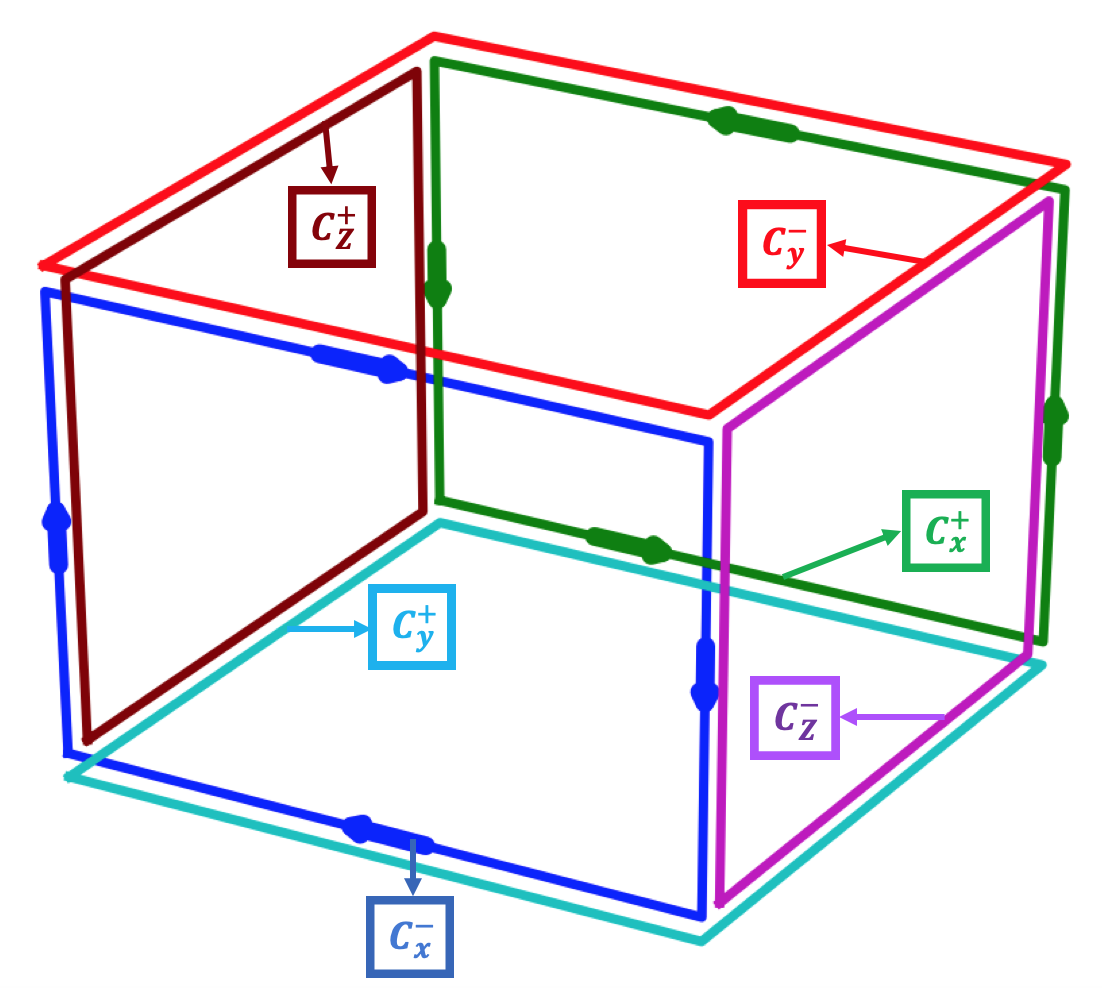
\includegraphics[scale=.28]{Images/c1_3}
        \caption{Current Direction in $C_x^{\pm}$}
        \label{fig:c1}
    \end{subfigure}%
    \begin{subfigure}{.5\linewidth}
        \centering
        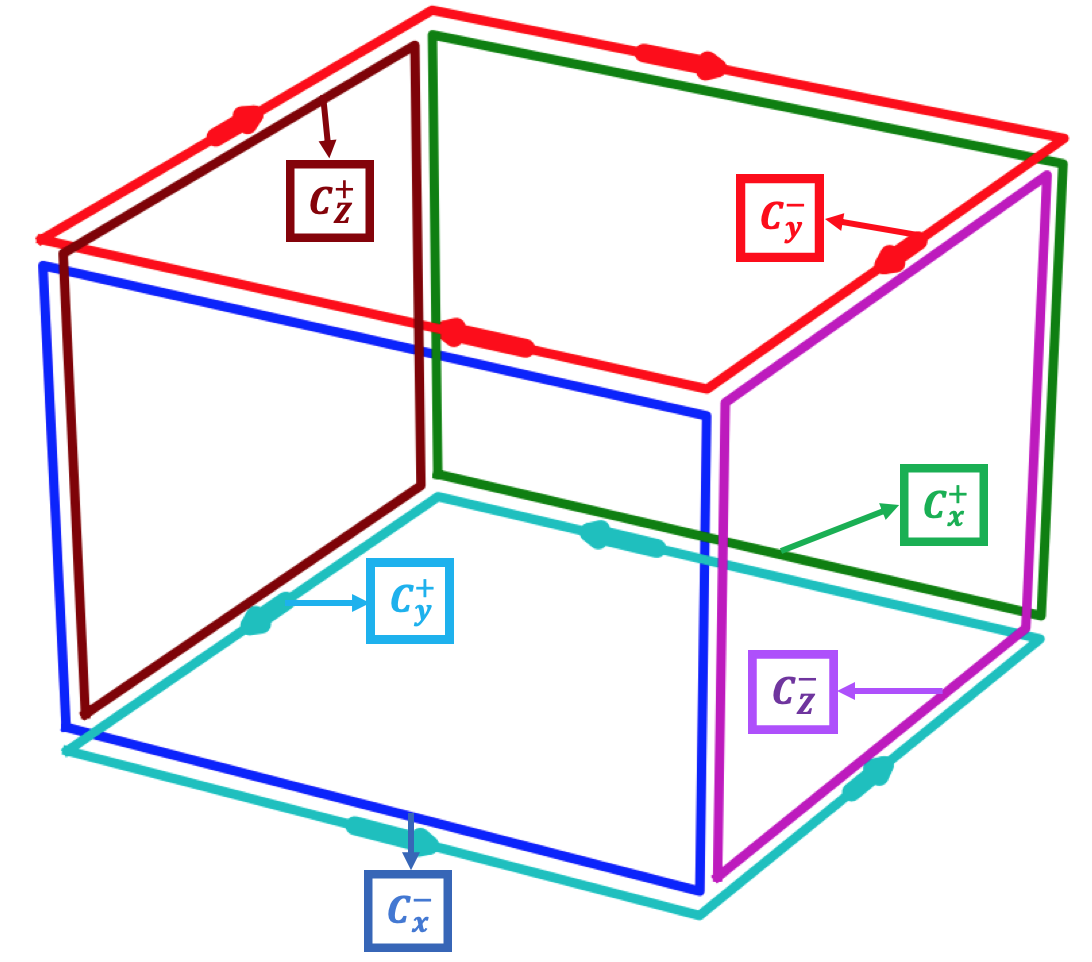
\includegraphics[scale=.28]{Images/c3_3}
        \caption{Current Direction in $C_y^{\pm}$}
        \label{fig:c3}
    \end{subfigure}\\[1ex]
    \begin{subfigure}{\linewidth}
        \centering
        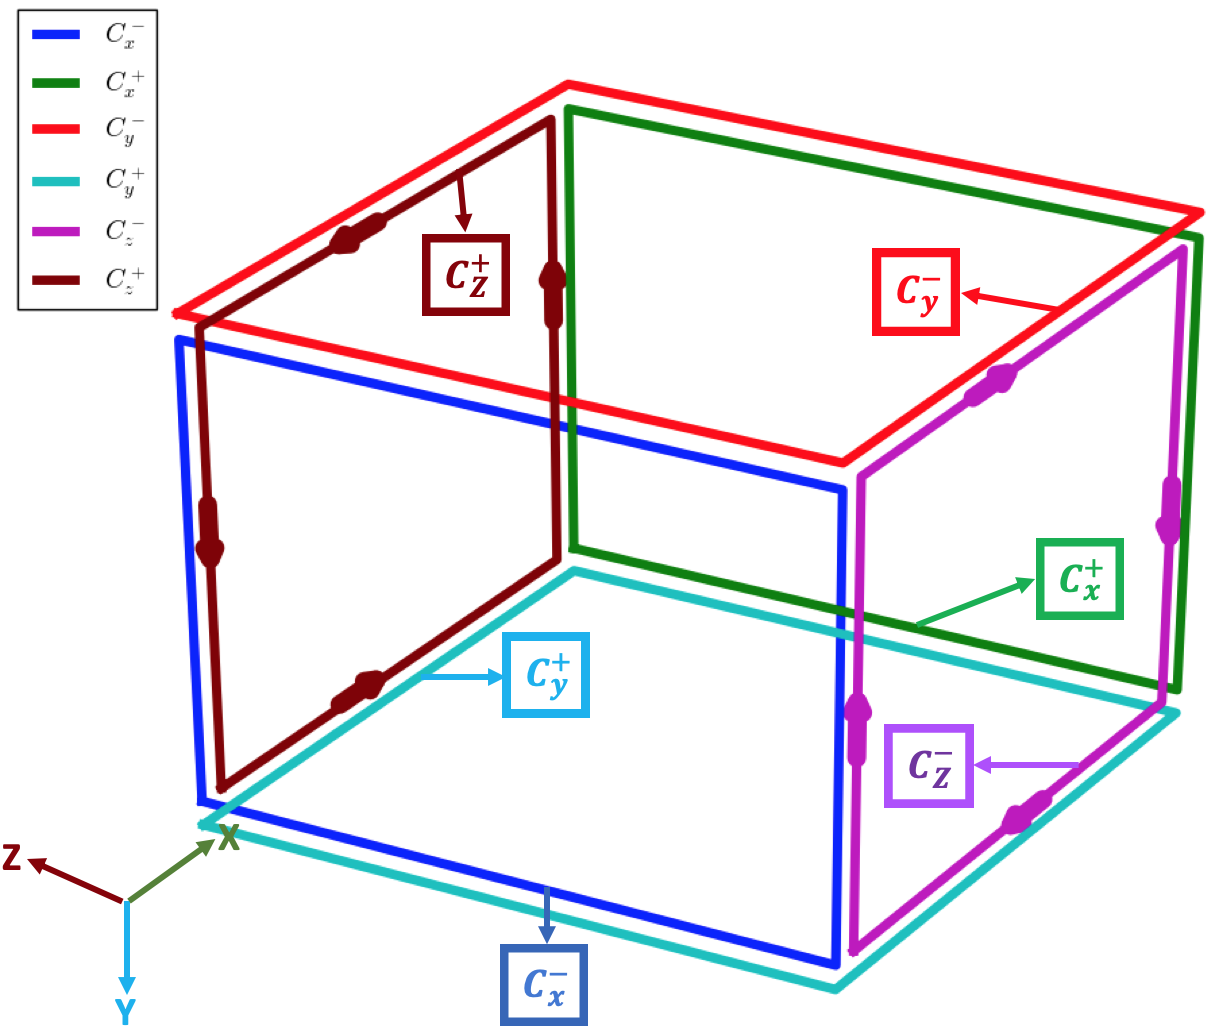
\includegraphics[scale=.33]{Images/c5_3}
        \caption{Current Direction in $C_z^{\pm}$}
        \label{fig:c5}
    \end{subfigure}

\caption[Singular currents corresponding to the singular value $\Sigma_{66}=0$]{Singular currents corresponding to the singular value $\Sigma_{66}=0$.  The currents are equal in magnitude but opposed in direction for each of (a) $C_x^{\pm}$, (b) $C_y^{\pm}$ and (c) $C_z^{\pm}$. When added, the net current (and hence field) is always zero, thus explaining the singular value of zero.}
    \label{fig:cDir}
\end{figure}

We can imagine the elements of the singular vector as describing
eigen-currents.  In row 6, this would describe a set of currents like
those depicted in Fig.~\ref{fig:cDir}.  In this case, if the coils all
overlap perfectly, as they do in this simulation, such a mode has a
net current of zero.  Hence, no matter what the total current applied
to this mode, it will never generate a magnetic field.  Hence the
singular value is always zero.

%\textcolor{red}{The higher frequency information is typically represented by the singular vectors corresponding to the smaller singular values. That is, with increase of n values the left and right singular vectors tend to have more sign changes. The consequence is that the SVD provides us with basis right singular vectors for an expansion where each basis vector represents a certain “frequency,” approximated by the number of times the entries in the vector change signs.}

%It can be as explained by Fig.~\ref{fig:cDir} where one of the coil current mode was shown for all six coils. The total current contribution is found to be zero due to current contributions from $C_x^{\pm}$ in Fig.~\ref{fig:cDir}\textcolor{blue}{(a)}, $C_y^{\pm}$ in Fig.~\ref{fig:cDir}\textcolor{blue}{(b)} and $C_z^{\pm}$ in Fig.~\ref{fig:cDir}\textcolor{blue}{(c)}.


On further inspection, the currents depicted in each of panels (a),
(b), and (c) of Fig.~\ref{fig:cDir} correspond to magnetic field
gradients $\partial B_x/\partial x$, $\partial B_y/\partial y$, and
$\partial B_z/\partial z$, respectively.  These gradients are not
independent of one another because, according to Maxwell's equations:
\begin{equation}
\frac{\partial B_x}{\partial x}+\frac{\partial B_y}{\partial y}+\frac{\partial B_z}{\partial z}=\vec{\nabla}\cdot\vec{B}=0.\label{eq:divb0}
\end{equation}
The problem of the singular value of zero can also be considered in
this differential form.  Consider coils which have been designed which
generate gradients $\partial B_x/\partial x$, $\partial B_y/\partial
y$, and $\partial B_z/\partial z$ near the origin of coordinates.  An
example of such a coil system would be three orthogonal anti-Helmholtz
coils.  If the first two coils are energized to produce uniform
gradients $\partial B_x/\partial x$, $\partial B_y/\partial y$, then
according to Eq.~(\ref{eq:divb0}) they necessarily also generate a
gradient in the $z$ direction
\begin{equation}
\frac{\partial B_z}{\partial z}=-\frac{\partial B_x}{\partial x}-\frac{\partial B_y}{\partial y}.\label{eq:dbzdz}
\end{equation}
The third coil, which generates $\partial B_z/\partial z$ is
therefore unnecessary.  Or conversely, if the third coil is included
in a three-dimensional feedback system, it is possible that the
control system will generate a current in the third coil which
mistakenly counteracts the effect of the other two coils.  This is
essentially what is happening in the case of the bad singular mode
described by Fig.~\ref{fig:cDir}.

Eq.~(\ref{eq:dbzdz}) suggests one method to prevent the problematic
coil mode from ever being excited: remove the coil which generates
$\partial B_z/\partial z$.  I implemented this in the Python
code by requiring that the currents in the $C_z^+$ and $C_z^-$ always
be in the same direction and have the same value, {\it i.e.}~like the
currents in a Helmholtz coil.  This means that there are only five
independently controlled currents, which I denote $C_x^+$, $C_x^-$,
$C_y^+$, $C_y^-$, and $C_z^\pm$.

\textcolor{red}{Need to add a note here about spherical harmonics. Need to add some note about Rawlik's patch coil system.  Or this could/should go in future work with a forward reference here.}

\textcolor{red}{Where to add Refs.~\cite{field_abel,field_jeff} ?}
%To break the mode, two out of
%the six coils have been wired together so that they can act as one
%resulting total compensation coils be five.
%It was found that due to this, the condition number is decreased drastically to 2.


% For the prototype, two different configuration of compensation coils have been exploited. In the first case, all the six coils have been used in the six faces surrounding the compensation area and for the later one, two coils have been wired together so that they can act as one making total five instead of six coils. The main reason for using the second configuration is the condition number of $\bm{M}$. It was found to be $\sim$4.7 for the second one as compared to $\sim$51 in the first.


%\textcolor{red}{Is Fig.~\ref{fig:matrix_patch_5c} required ????}

\fig{Images/matrix_patch_5c}{width = \textwidth}{
Color map of $M_{sc}$ elements for 24 fluxgate axes and 5 coils. Coil
dimensions and fluxgate positions are the same as for
Fig.~\ref{fig:matrix_patch_6c}.\label{fig:matrix_patch_5c}}{Matrix for
5 coils.}

The simulated matrix $\bm{M}$ for this configuration is shown in
Fig.~\ref{fig:matrix_patch_5c}.  Naively, it is not considerably
different that the corresponding matrix for six coils, which was
displayed in Fig.~\ref{fig:matrix_patch_6c}.  However, upon performing
the singular value decomposition, the differences become evident.



\fig{Images/Diag_patch_5c}{width = \textwidth}{
Color map of diagonal matrix $\bm{\Sigma}$ found by SVD of $\bm{M}$ for 24 fluxgate axes and 5 coils. \label{fig:diag_patch_5c}}{Diagonal Matrix for 5 coils.}

Fig.~\ref{fig:diag_patch_5c} displays the $\bm{\Sigma}$ matrix
resulting from singular value decomposition.  This results in five
singular values, one for each coil mode.  Most importantly, the
singular value which was zero has been removed from the matrix.  The
remaining singular values are now also all of similar order of
magnitude.  The condition number of the matrix is 2.01, which is a
considerable improvement compared to the infinite condition number of
the six-coil system.

\fig{Images/Right_patch_5c}{width = \textwidth}{Color map of orthogonal matrix $\bm{V^T}$ found by SVD of $\bm{M}$ 24 fluxgate axes and 5 coils. \label{fig:right_patch_5c}}{Orthogonal matrix $\bm{V^T}$ for 5 coils.}

The matrix of right singular vectors $\bm{V^T}$ is displayed in
Fig.~\ref{fig:right_patch_5c}.  The uniform field modes are clearly
visible in rows 1, 3, and 4, corresponding to Helmholtz-like singular
current modes.  Two gradient modes also appear in rows 2 and 5, which
are different combinations of the anti-Helmholtz-like gradients in
each of the $x$ and $y$ directions.

\textcolor{red}{Say that we also made a PI simulation and it worked better.  Should probably say this at the end of this section.}


\begin{table} [htb!]
    \centering
    \begin{tabular} { |c|c|c|c|c|c|} 
        \hline
        Coils & \makecell{Matrix \\Condition Number} &\makecell{Inverse Matrix \\ Condition Number} & \makecell{Regularization \\Parameter, $r$}\\
        \hline\hline
        \makecell{$C_x^-$, $C_x^+$, $C_y^-$,\\ $C_y^+$, $C_z^-$ and $C_z^+$ } & 26.37 & 1.71 & 3.04 \\ 
        \hline
        \makecell{$C_x^{\pm}$, $C_y^-$, $C_y^+$,\\ $C_z^-$ and $C_z^+$ } & 2.26 & 1.08 & 3.6 \\         
        \hline
        \makecell{$C_x^-$, $C_x^+$, $C_y^\pm$,\\ $C_z^-$ and $C_z^+$ } & 2.27 & 1.09 & 3.62 \\
        \hline
        \makecell{$C_x^-$, $C_x^+$, $C_y^-$,\\ $C_y^+$ and $C_z^\pm$ } & 2.41 & 1.10 & 3.56 \\
        \hline

    \end{tabular}
    % \vspace{4mm}
    \caption[Properties for different coil configurations]{Matrix properties for different 6- and 5-coil configurations for fluxgate sensors at 1, 3, 6 and 8.}\label{table:mcond_coil}
\end{table}


I then implemented this solution into the active magnetic compensation
system.  Rather than physically wire two coils together, I implemented
a software solution where the currents in one pair of opposing coils
were required to be equal and run in the same direction.

The results of matrix measurement followed by singular value
decomposition are shown in Table~\ref{table:mcond_coil}.  Since I
could only instrument $4\times 3$ fluxgate axes, only such matrices
are considered.  The measurements were done with no magnetic shield
inside the coil cube~\textcolor{red}{and I think they'd be the same if
we had a shield present, maybe.  Need to firm up this statement.}

Table~\ref{table:mcond_coil} shows that the condition number of the
matrix is reduced by more than a factor of ten when comparing the
six-coil solution to the five-coil solution.  Configurations where
opposing coils in the $x$, $y$, and $z$ directions are alternately
selected for the Helmholtz-like current configuration in the five-coil
solution.  Table~\ref{table:mcond_coil} shows that any of these
configurations gave essentially the same results for the condition
number.

Clearly, in the six-coil case, it is an absolute necessity to
regularize the matrix, which as I discussed early may be done by
adjusting the regularization parameter to minimize the condition
number of the Tikhonov regularized pseudoinverse.  I decided also to
study Tikhonov regularization for the five-coil case, to see if it had
any impact on the PI feedback system.  Results of the Tikhonov
regularization process are also displayed in
Table~\ref{table:mcond_coil}.

% \fig{Images/coil_reg}{width = \textwidth,height=12cm}{Currents (left vertical axis) in all six coil sides ($C_x^\pm$, $C_y^\pm$ and $C_z^\pm$) with drift $\Delta B$ (right vertical axis) at 12 sensor positions with fluxgate positions 1, 3, 6 and 8 for $k_c^p$=0.0, $k_c^i$=1.0 (see Eq.~(\ref{eq:I})). The $r$=2.9 in (a) and $r$=3.39 in (b). For position of coils and fluxgates see Fig.~\ref{fig:coil}. All grey color curves in $\Delta B$ graph denote the drift in signal that would have been without the compensation while all other color curves denote the actual drift in signal at all 12 sensor positions found by Eq.~(\ref{eq:del_B}). Vertical dashed lines indicate the time of the perturbation coil being turned on and off. The current supplied on perturbation coil was 10  mA. The resolution index 1 (see Table~\ref{table:t7freq}) with 50 no of averages per measurement used. The loop sampling frequency was found to be $\sim$6.5 Hz.\label{fig:coil_reg}}{Coil currents with drift $\Delta B$ for different coil configuration in regularized $\bm{M^{-1}}$}
\fig{Images/coil_reg4}{width = \textwidth,height=12cm}{Currents (left) in all six coils ($C_x^\pm$, $C_y^\pm$ and $C_z^\pm$) and field change $\Delta B$ (right). The fluxgate positions are 1, 3, 6 and 8.  The feedback parameters are $k_c^p=0.0$, $k_c^i=1.0$.  The current supplied to the perturbation coil was 10  mA when switch on. Resolution index 1 with 50 averages per cycle were used. The matrix condition number is 26.37 in (a) which while inverse for $r$=3.04 gives 1.71 and The matrix condition number is 2.26 in (b) which while inverse for $r$=3.6 gives 1.08.\label{fig:coil_reg}}{Coil currents with field change $\Delta B$ for different coil configuration in regularized $\bm{M^{-1}}$}



% \fig{Images/coil_pseudo}{width = \textwidth,height=12cm}{Currents (left vertical axis) in all six coil sides ($C_x^\pm$, $C_y^\pm$ and $C_z^\pm$) with drift $\Delta B$ (right vertical axis) at 12 sensor positions with fluxgate positions 1, 3, 6 and 8 for $k_c^p$=0.0, $k_c^i$=1.0 (see Eq.~(\ref{eq:I})). Pseudoinverse was used in both case. For position of coils and fluxgates see Fig.~\ref{fig:coil}. All grey color curves in $\Delta B$ graph denote the drift in signal that would have been without the compensation while all other color curves denote the actual drift in signal at all 12 sensor positions found by Eq.~(\ref{eq:del_B}). Vertical dashed lines indicate the time of the perturbation coil being turned on and off. The current supplied on perturbation coil was 10  mA. The resolution index 1 (see Table~\ref{table:t7freq}) with 50 no of averages per measurement used. The loop sampling frequency was found to be $\sim$6.5 Hz.\label{fig:coil_pseudo}}{Coil currents with drift $\Delta B$ for different coil configuration in non-regularized $\bm{M^{-1}}$}

\fig{Images/coil_pseudo3}{width =\textwidth,height=12cm}{
Currents (left) in all six coils ($C_x^\pm$, $C_y^\pm$ and $C_z^\pm$)
and field change $\Delta B$ (right). The fluxgate positions are 1, 3,
6 and 8. Pseudoinverse was used in both case.  The feedback parameters
are $k_c^p=0.0$ and $k_c^i=1.0$.  The current supplied to the
perturbation coil was 10 mA when switch on. Resolution index 1 with 50
averages per cycle were used.\label{fig:coil_pseudo}}{Coil currents
with field change $\Delta B$ for different coil configuration in
non-regularized $\bm{M^{-1}}$}


\FloatBarrier
\subsection{Extra Data}
\fig{Images/i_rm_comb}{width = \textwidth}{.. \label{fig:i_r_comb}}{S}

\fig{Images/matrix_comb}{width = \textwidth}{.. \label{fig:matrix_comb}}{S}

\fig{Images/diag_comb}{width = \textwidth}{.. \label{fig:diag_comb}}{S}

\fig{Images/right_comb}{width = \textwidth}{.. \label{fig:right_comb}}{S}

\fig{Images/5c_x}{width = \textwidth}{$C_x^{\pm}$, $C_y^-$, $C_y^+$, $C_z^-$ and $C_z^+$. \label{fig:5c_x}}{S}

\fig{Images/5c_x_all}{width = \textwidth}{$C_x^{\pm}$, $C_y^-$, $C_y^+$, $C_z^-$ and $C_z^+$. \label{fig:5c_x_all}}{S}
 
\fig{Images/5c_y}{width = \textwidth}{$C_x^-$, $C_x^+$, $C_y^\pm$, $C_z^-$ and $C_z^+$ . \label{fig:5c_y}}{S}

\fig{Images/5c_y_all}{width = \textwidth}{$C_x^-$, $C_x^+$, $C_y^\pm$, $C_z^-$ and $C_z^+$. \label{fig:5c_y_all}}{S}
\fig{Images/5c_z}{width = \textwidth}{$C_x^-$, $C_x^+$, $C_y^-$, $C_y^+$ and $C_z^\pm$. \label{fig:5c_z}}{S}

\fig{Images/5c_z_all}{width = \textwidth}{$C_x^-$, $C_x^+$, $C_y^-$, $C_y^+$ and $C_z^\pm$. \label{fig:5c_z_all}}{S}



\begin{table} [htb!]
    \centering
    \begin{tabular} { |c|c|c|c|c|c|} 
        \hline
        Coils & \makecell{Matrix \\Condition Number} &\makecell{Inverse Matrix \\ Condition Number} & \makecell{Regularization \\Parameter, $r$}\\
        \hline\hline
        \makecell{$C_x^-$, $C_x^+$, $C_y^-$,\\ $C_y^+$, $C_z^-$ and $C_z^+$ } & 26.37 & 1.71 & 3.04 \\ 
        \hline
        \makecell{$C_x^{\pm}$, $C_y^-$, $C_y^+$,\\ $C_z^-$ and $C_z^+$ } & 2.26 & 1.08 & 3.6 \\         
        \hline
        \makecell{$C_x^-$, $C_x^+$, $C_y^\pm$,\\ $C_z^-$ and $C_z^+$ } & 2.27 & 1.09 & 3.62 \\
        \hline
        \makecell{$C_x^-$, $C_x^+$, $C_y^-$,\\ $C_y^+$ and $C_z^\pm$ } & 2.41 & 1.10 & 3.56 \\
        \hline
        \makecell{$C_x^-$, $C_x^+$+$C_y^-$,\\ $C_y^+$, $C_z^-$ and $C_z^+$ } & 2.97 & 1.14 & 3.6 \\
        \hline
        \makecell{$C_x^-$, $C_x^+$,$C_y^-$,\\ $C_y^+$+$C_z^-$ and $C_z^+$ } & 2.8 & 1.14 & 3.62 \\
        \hline
        \makecell{$C_x^-$+$C_y^-$, $C_x^+$,\\ $C_y^+$,$C_z^-$ and $C_z^+$ } & 25 & 1.69 & 3.06 \\
        \hline
        \makecell{$C_x^-$, $C_x^+$+$C_y^+$,\\ $C_y^-$, $C_z^-$ and $C_z^+$ } & 25 & 1.70 & 3.05 \\
        \hline
        \makecell{$C_x^-$, $C_x^+$, $C_y^+$,\\ $C_y^-$+$C_z^-$ and $C_z^+$ } & 26.14 & 1.65 & 3.06 \\
        \hline
        \makecell{$C_x^-$+$C_x^+$, $C_y^-$+ $C_y^+$,\\$C_z^-$ and $C_z^+$ } & 440.57 & 1.79 & 2.54 \\
        \hline
        \makecell{$C_x^-$+$C_x^+$, $C_y^-$+ $C_y^+$,\\ and $C_z^-$+$C_z^+$ } & 1.27 & 1.0 & 3.73 \\
        \hline

    \end{tabular}
    % \vspace{4mm}
    \caption[Properties for different coil configurations]{Matrix properties for different 6- and 5-coil configurations for fluxgate sensors at 1, 3, 6 and 8.}\label{table:mcond_coi2}
\end{table}

\section{Future Section ??}\label{sec:metrics_res}

\subsection{Experimental Current Error and Remaining Fluctuation}

\begin{itemize}
\item Basic message of Fig. 5.4 is that experiment and simulation kind of agree.
% \item In simulation a set of twelve $B_s^\text{rand}$ has been generated by normal distribution around zero with standard deviation being 1.5 nT.
% % \item In experiment  set of twelve $B_s^\text{rand}$ has been generated by magnetic field signals from fluxgate positions at 1, 2 and 7 using Eq.~(\ref{eq:del_B}). For position of the fluxgates please see Fig.~\ref{fig:coil}.
% \item $r$ has been varied from 0 to 6 in an increment of 0.29 and for each $r$, PI control algorithm has been implemented for n measurements and for every measurements, signals from fluxgates at positions 1,2 and 7 are stored as $B_{\text{meas}}$ and uncompensated B field has been stored as $B_{\text{uncomp}}$ using  $B_{\text{meas}}-\bm{M}(I_c^n-I_c^0)$ where $I_c^n$ can be found using Eq.~(\ref{eq:I}). From those stored values,  Eq.~(\ref{eq:B_coils-sim}) has been found by $B_{\text{meas}}^{\text{max}}(r)-B_{\text{meas}}^{\text{min}}(r)$ and $B_s^\text{rand}$ has been found by $B_{\text{uncomp}}^{\text{max}}(r)-B_{\text{uncomp}}^{\text{min}}(r)$ and $\Delta I_c^{\text{exp}}(r)$ has been found using same as Eq.(\ref{eq:del_Is}). 
\end{itemize}

\fig{Images/mont_exp}{width = \textwidth}{The effect of $r$ on (a) current error  and (b) remaining field fluctuations in experimental setup for $k_c^p=1.0$ for fluxgate signals from 1, 2 and 7. Here, 100 mA current has been supplied in the perturbation coil. For position of the fluxgates  and coil see Fig.~\ref{fig:coil}.\label{fig:mont_comp}}{The effect of $r$ for experimental setup.}

The effect of $r$ on the current error and remaining field fluctuations in experimental setup for fluxgate signals from 1, 2 and 7 are shown in Fig.~\ref{fig:mont_comp}. For position of the sensors please see Fig.~\ref{fig:coil}. For data measurement, for certain loops, PI control algorithm with $k_c^p=$1.0 and $k_c^i=$0.0 has been implemented for $r$ ranges from 0 to 6 in an increment of 0.29. For every measurements, signals from fluxgates at positions 1,2 and 7 are stored as $B_{\text{meas}}$ and uncompensated B field has been stored as $B_{\text{uncomp}}$ which is predicted by Eq.~\ref{eq:Buncomp}. The difference between maximum value of $B_{\text{uncomp}}$ and $B_{\text{uncomp}}$ will give the field fluctuation due to 100 mA supplied in rhe perturbation coil. Moreover, the difference between maximum value of $B_{\text{meas}}$ and $B_{\text{meas}}$ will give the amount of compensation of the field which when equal to field fluctuation indicates no compensation. The ratio of rms value of this to the field fluctuation will generate the remaining fluctuation $F$ which is shown for different $r$ in Fig.~\ref{fig:mont_comp}\textcolor{blue}{(b)}. It is seen that for a particular filed perturbation, the remaining fluctuation is $\approx$0.45 which indicates that the maximum correction is $\mathbf{(1-0.45)\times100\%=55\%}$. Moreover, $\Delta I_c^{\text{exp}}(r)$ has been found using Eq.(\ref{eq:del_Is}) and the rms has been determined which is shown in  Fig.~\ref{fig:mont_comp}\textcolor{blue}{(a)}. It is seen that around 100 mA rms of current array is required to compensate the perturbation which eventually vanishes with $r$ increment as expected.
% We have studied the coil current response and magnetic fluctuation reduction in

% In Section~\ref{sec:inv}, we have already talked about how the regularization parameter $r$ came into effect. Then, in Section~\ref{sec:mont}, regularization by random magnetic distribution method has been described which has been taken from Ref.~\cite{bea} where a suitable value of $r$ has been found which will give the best compromise between the magnetic field fluctuation and coil current fluctuation. We have generated a fluctuation by our perturbation coil. $r$ has been varied from 0 to 6 in an increment of 0.29 and for each $r$, PI control algorithm has been implemented for n measurements and for every measurements, signals from fluxgates at positions 1,2 and 7 are stored as $B_{\text{meas}}$ and uncompensated B field has been stored as $B_{\text{uncomp}}$ using  $B_{\text{meas}}-\bm{M}(I_c^n-I_c^0)$ where $I_c^n$ can be found using Eq.~(\ref{eq:I}). From those stored values,  Eq.~(\ref{eq:B_coils-sim}) has been found by $B_{\text{meas}}^{\text{max}}(r)-B_{\text{meas}}^{\text{min}}(r)$ and $B_s^\text{rand}$ has been found by $B_{\text{uncomp}}^{\text{max}}(r)-B_{\text{uncomp}}^{\text{min}}(r)$ and $\Delta I_c^{\text{exp}}(r)$ has been found using same as Eq.(\ref{eq:del_Is}). 

% The root mean square (RMS) of $\Delta I_c^{\text{exp}}(r)$ is calculated as
% \begin{equation}\label{eq:delta_Iexp_rms}
%      \Delta I_{\text{RMS}}^{\text{exp}}(r)= \sqrt{\frac{1}{6}\sum_{c=1}^6 (\Delta I_c^{\text{exp}}(r))^2}
% \end{equation}
% The remaining fluctuation is calculated as
% \begin{equation}\label{eq:fluc}
%     F(r)=\frac{\sqrt{\frac{1}{12} \sum_{s=1}^{12} (B_s^{\text{sim}}(r))^2}}{\sqrt{\frac{1}{12} \sum_{s=1}^{12} (B_s^{\text{rand}}(r))^2}}
% \end{equation}
% The field without compensation is predicted by 
% \begin{equation}
    
% \end{equation}
% In this Section, we have found Eq.~(\ref{eq:delta_Isim_rms}) and Eq.~(\ref{eq:fluc}) in experimental setup.
% $B_s^{\text{rand}}$ will be replaced by
% The fluctuation caused by perturbation coil is
% \begin{equation}\label{eq:B_coils-exp}
%     B_s^{\text{fluc}}(r) =B_{\text{uncomp}}^{\text{max}}(r)-B_{\text{uncomp}}^{\text{min}}(r)
% \end{equation}
% To compensate the fluctuation
% \begin{equation}\label{eq:B_coils-exp}
%     B_s^{\text{exp}}(r) =B_{\text{meas}}^{\text{max}}(r)-B_{\text{meas}}^{\text{min}}(r)
% \end{equation}


% \begin{equation}\label{eq:fluc_exp}
%     F(r)=\frac{\sqrt{\sum_s \frac{1}{s}(B_{\text{meas}}^{\text{max}}(r)-B_{\text{meas}}^{\text{min}}(r))^2}}{\sqrt{\sum_s \frac{1}{s}(B_{\text{uncomp}}^{\text{max}}(r)-B_{\text{uncomp}}^{\text{min}}(r))^2}}
% \end{equation}

% In Section~\ref{sec:mont}, 30 different sets of random magnetic field ($B_s^{\text{rand}}$) values have been chosen with center of distribution being 0 and standard deviation 5 nT for 12 different fluxgate sensor positions whose labels are given in the horizontal axis of Fig.~\ref{fig:m} and the positions are specified in Fig.~\ref{fig:coil}. Here, we have chosen one out of the 30 different sets of $B_s^{\text{rand}}$ and go through the steps as in Section~\ref{sec:mont} to generate similar figures like in Fig.~\ref{fig:Isim}, Fig.~\ref{fig:fluc-sim} and Fig.~\ref{fig:I-fluc}. For the experimental setup, we have done the similar steps to generate those figures except instead of generating $B_s^{\text{rand}}$ randomly, we have applied current in the perturbation coil to generate the required drift ( see Eq.~(\ref{eq:del_B}) ) which will be treated as $B_s^{\text{rand}}$. The results of the simulation as well as experiment are given in Fig.~\ref{fig:mont_comp}, where Fig.~\ref{fig:mont_comp}\textcolor{blue}{(a)}, Fig.~\ref{fig:mont_comp}\textcolor{blue}{(b)} and Fig.~\ref{fig:mont_comp}\textcolor{blue}{(c)} are the results found from simulation and Fig.~\ref{fig:mont_comp}\textcolor{blue}{(d)}, Fig.~\ref{fig:mont_comp}\textcolor{blue}{(e)} and Fig.~\ref{fig:mont_comp}\textcolor{blue}{(f)} are the results found from experiment. They are described in detail in Fig.~\ref{fig:Isim}, Fig.~\ref{fig:fluc-sim} and Fig.~\ref{fig:I-fluc}. It is seen that the experimental counterpart of each of the simulation that is Fig.~\ref{fig:mont_comp}\textcolor{blue}{(a)} of simulation is comparable to Fig.~\ref{fig:mont_comp}\textcolor{blue}{(d)} of experiment. Similarly, Fig.~\ref{fig:mont_comp}\textcolor{blue}{(b)} of simulation with Fig.~\ref{fig:mont_comp}\textcolor{blue}{(e)} of experiment and Fig.~\ref{fig:mont_comp}\textcolor{blue}{(c)} of simulation with Fig.~\ref{fig:mont_comp}\textcolor{blue}{(f)} of experiment are comparable and they produce similar results. The similar results of the simulation with experiment justifies the the simulation model described in Section~\ref{sec:mont}.

% \fig{Images/mont_comp3}{width = \textwidth,height =10cm}{Simulation result for one set of $B_s^{\text{rand}}$ for the Fig.~\ref{fig:Isim}, Fig.~\ref{fig:fluc-sim} and Fig.~\ref{fig:I-fluc} are shown in (a), (b) and (c) and corresponding experimental results are in (d), (e) and (f). For the description of the figures see the text in Fig.~\ref{fig:Isim}, Fig.~\ref{fig:fluc-sim} and Fig.~\ref{fig:I-fluc}. For position of fluxgate sensors see Fig.~\ref{fig:coil}.\label{fig:mont_comp}}{Short}



% The above results in Fig.~\ref{fig:mont_comp}, where simulation results are similar to experimental one justify the simulation method described in Section~\ref{sec:mont}. The upcoming Section is all about P and I term (see Eq.~(\ref{eq:I}) ) behaviour. 
% \fig{Images/sf6p}{width = \textwidth}{p127, 100mA stimulus,p0.7,r3.5,Simulation result for one set of $B_s^{\text{rand}}$ for the Fig.~\ref{fig:Isim}, Fig.~\ref{fig:fluc-sim} and Fig.~\ref{fig:I-fluc} are shown in (a), (b) and (c) and corresponding experimental results are in (d), (e) and (f). For the description of the figures see the text in Fig.~\ref{fig:Isim}, Fig.~\ref{fig:fluc-sim} and Fig.~\ref{fig:I-fluc}. For position of fluxgate sensors see Fig.~\ref{fig:coil}.\label{fig:adev}}{Short}
\fig{Images/sf6sr}{width = \textwidth}{Allan deviation and shielding factor for fluxgate positions 1, 3, 6 and 8. For position of fluxgate sensors see Fig.~\ref{fig:coil}.\label{fig:adev}}{Allan deviation and shielding factor.}

\fig{Images/center}{width = \textwidth}{The effect on the control sensors signal fluctuations for PI control algorithm at fluxgate positions 1, 3, 6 and 8. For position of fluxgate sensors see Fig.~\ref{fig:coil}.\label{fig:center}}{The effect on the control sensors signal fluctuations.}
